\section{Finite difference schemes} \label{sec:finitedifferencesschemes}
\subsection{Overview}
Previously, we considered the pricing problem of American options which requires solving the free boundary problem defined in \eqref{eq:blackscholes:preliminaries:american_options_pde_free_boundary_problem_full}.
Then, we presented the front fixing method as a strategy to fix the moving boundary using a change of variable. Moreover, we derived the PDEs for call and put options that resulted from transforming \eqref{eq:blackscholes:preliminaries:american_options_pde_free_boundary_problem_full} using the change of variable suggested by Nielsen et al.\cite{nielsen_2001}, and by Company et al.\cite{company_egorova_jodar_2014} which resulted in the systems \eqref{eq:blackscholes:frontfixingmethod:nielsen:american_options_bs_pde} and \eqref{eq:blackscholes:frontfixingmethod:logtransform:american_options_bs_pde}, respectively. Now, we present numerical schemes for solving \eqref{eq:blackscholes:frontfixingmethod:nielsen:american_options_bs_pde}. But before we jump into that, we define what it means to compute a numerical solution to a PDE problem.

Recall that the solution $v(x,t)$ of 
\eqref{eq:blackscholes:frontfixingmethod:nielsen:american_options_bs_pde} is defined in the continuous region 
\begin{subequations}
  \label{eq:finitedifferencesschemes:overview:continous_domain}
\begin{align}
  \text{\textbf{Call:}} \qquad& \mathcal{T}: [0, T], \qquad \mathcal{X}: [0, 1], \qquad  \mathcal{F}: \mathcal{X} \times \mathcal{T} \\
  \text{\textbf{Put:}} \qquad& \mathcal{T}:[0, T], \qquad \mathcal{X}:[1, \infty), \qquad \mathcal{F}: \mathcal{X} \times \mathcal{T},
\end{align}
\end{subequations}
Suppose we discretize $\mathcal{F}$ into the grid $\mathcal{G}$ (See figure \ref{eq:finitedifferencesschemes:overview:grid}) with $N+1$ and $M+1$ nodes
\begin{align}
  \label{eq:finitedifferencesschemes:overview:grid}
  \mathcal{G} := \{(x_i, t_n): (i, n) \in \{0,\dots,M+1\}\times\{0,\dots,N+1\}\}
\end{align}
where
\begin{align}
  \label{eq:finitedifferencesschemes:overview:grid_2}
  x_i &:= x_{\text{min}} + i\Delta x &  \qquad \text{for $i = 0,\dots, M+1$} \\
  t_n &:= t_{\text{min}} + i{\Delta t} & \qquad \text{for $i = 0,\dots, N+1$} \\
  \Delta{x} &:= \dfrac{x_{\text{max}} - x_{\text{min}}}{M+1} \\ 
  \Delta{t} &:= \dfrac{t_{\text{max}} - t_{\text{min}}}{N+1}
\end{align}
Each contiguous node in $\mathcal{G}$ will be separated by $\Delta{x}$ on the spatial axis and $\Delta{t}$ on the temporal axis. As $\Delta{x}$ and $\Delta{t}$ decreases, the number of nodes in the grid grows. Therefore, we refer to $\Delta{x}$ and $\Delta{t}$ as the resolution of the grid.
\begin{figure}[H]
  \label{fig:finitedifferencesschemes:overview:grid}
  \centering
  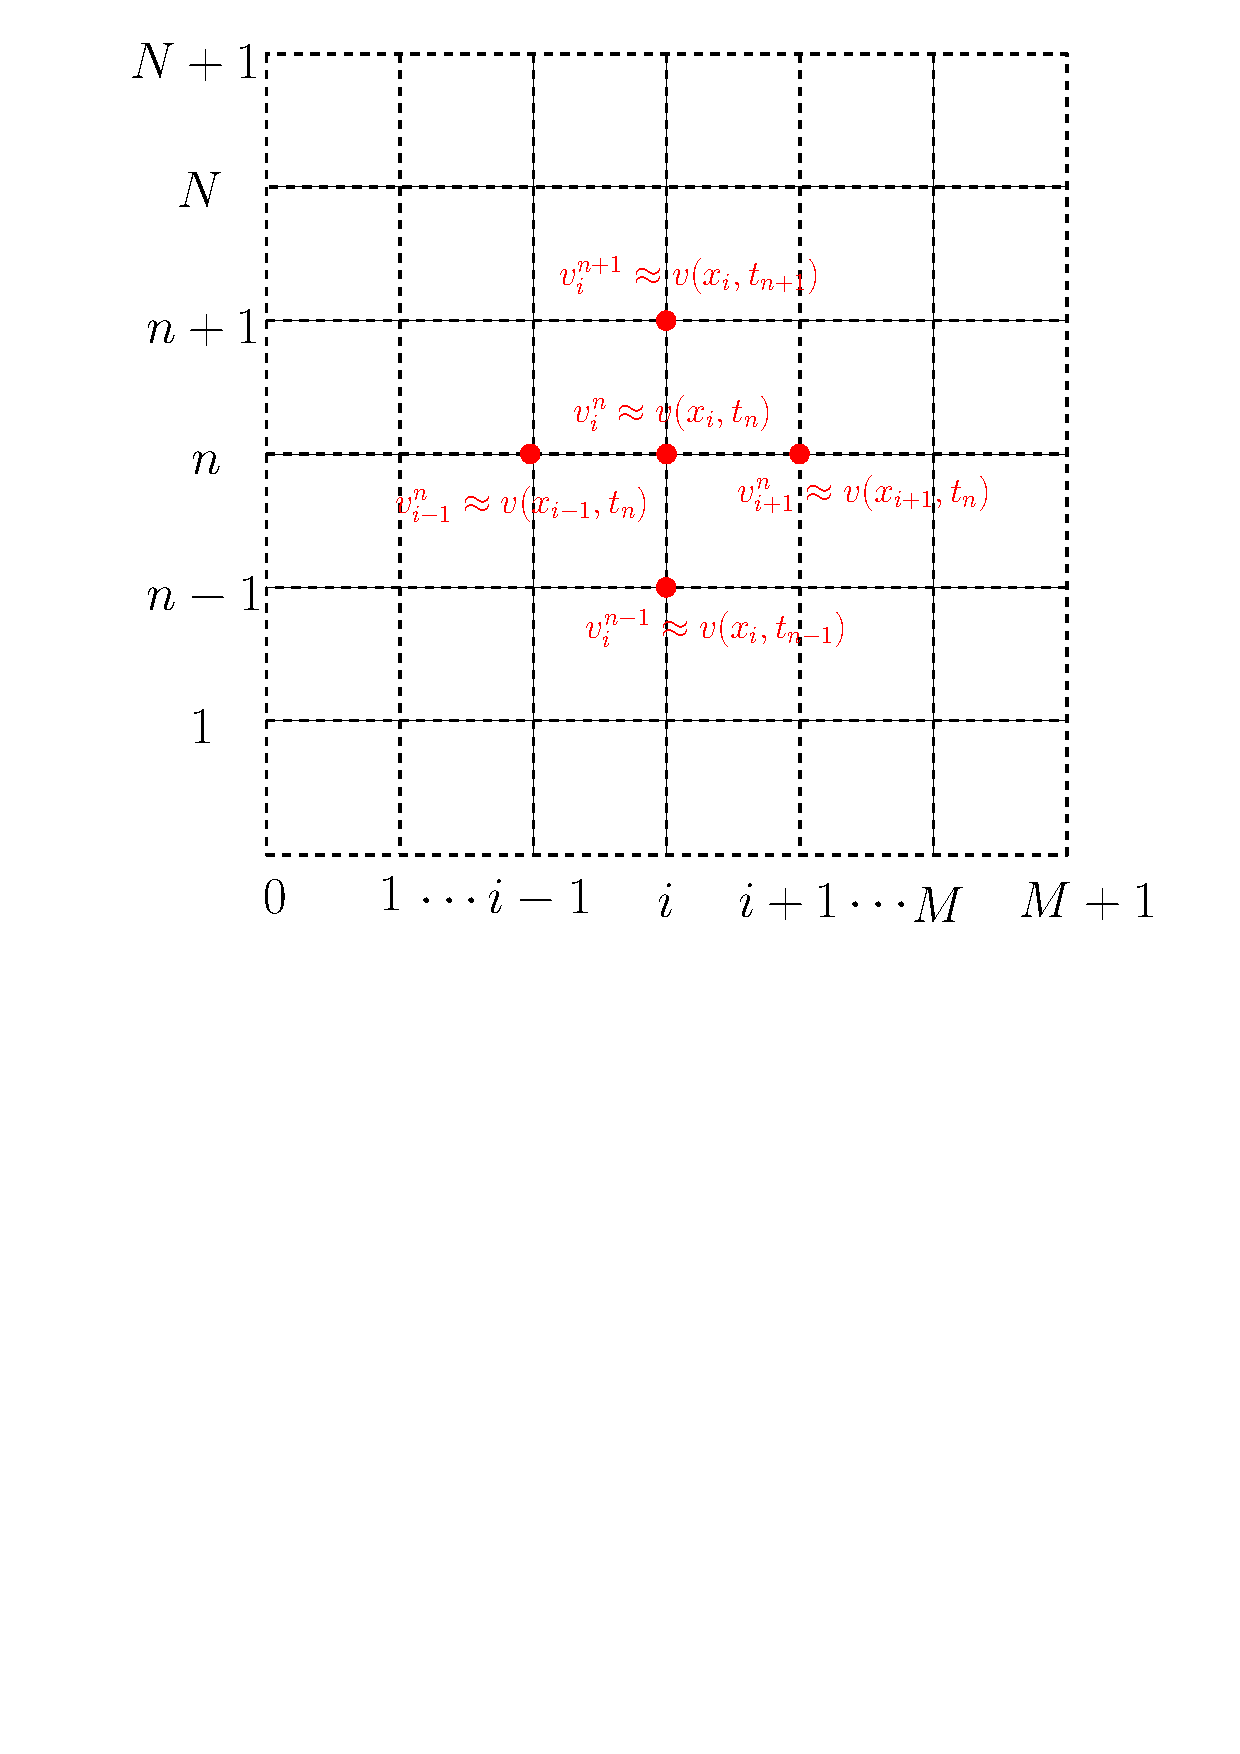
\includegraphics[scale=0.5]{chapters/chapter3/GridAproximation.pdf}
  \caption{The grid $\mathcal{G}$ and the approximation $v^{n}_{i} \approx v(x_i, t_n)$ in each node.}
\end{figure}
From equation \eqref{eq:finitedifferencesschemes:overview:continous_domain}, it is clear that $t_\text{min} = 0$ and $t_\text{max}=T$. Moreover, for call options, $x_\text{min} = 0$ and $x_\text{max}=1$. Likewise, for put options, $x_\text{min}=1$ and $x_\text{max}=x_\infty$ where $x_\infty$ is arbitrary large value. Given the grid $\mathcal{G}$, our goal is to approximate the value function $v(x, t)$ and the optimal exercise price $\bar{S}(t)$ at each node $(i, t)$
\begin{align*}
  v^{n}_i \approx v(x_i,t_n), \quad \bar{S}^{n} \approx \bar{S}(t_n)
\end{align*}
Moreover, we want that the error of the approximation converges to zero as we decrease the discretization parameters. Specifically, we want that the approximation error at each node 
\begin{align}
  \label{eq:finitedifferencesschemes:overview:local_truncation_error}
  e^{n}_i := v^{n}_i-v(x_i, t_n)
\end{align}
goes to zero as $\Delta{x}$ and $\Delta{t}$ decrease. Finally, within the grid we can approximate derivatives using is finite differences\cite{nassif2016introduction}. The idea of finite differences is to approximate derivatives as the difference of contiguous nodes in the grid $\mathcal{G}$. Let us say we are at node $(x_i, t_n)$, then the forward differences approximate the derivative as
\begin{align}
  \label{eq:finitedifferencesschemes:overview:forward_difference}
 \dfrac{v(x_{i+1},t_n) - v(x_{i}, t_n)}{\Delta{x}} = \dfrac{\partial{v}}{\partial{x}}(x_i, t_n) + O(\Delta{x})
\end{align}
the backward difference approximate the derivative as 
\begin{align}
  \label{eq:finitedifferencesschemes:overview:backward_difference}
  \dfrac{v(x_{i},t_n) - v(x_{i-1}, t_n)}{\Delta{x}} = \dfrac{\partial{v}}{\partial{x}}(x_i, t_n) + O(\Delta{x})
\end{align}
the central finite difference approximate the first order derivative as 
\begin{align}
  \label{eq:finitedifferencesschemes:overview:first_order_central_difference}
  \dfrac{v(x_{i+1},t_n) - v(x_{i-1}, t_n)}{2\Delta{x}} = \dfrac{\partial{v}}{\partial{x}}(x_i, t_n) + O(\Delta{x}^2)
 \end{align}
and the second order central difference approximate second order derivatives as
\begin{align}
  \label{eq:finitedifferencesschemes:overview:second_order_central_difference}
  \dfrac{v(x_{i+1},t_n) - 2v(x_i,t_n) + v(x_{i-1}, t_n)}{\Delta{x}^2} = \dfrac{\partial^2{v}}{\partial{x^2}}(x_i, t_n) + O(\Delta{x}^2)
 \end{align}
where $O(\Delta{x})$ and $O(\Delta{x}^2)$ are high order terms (See Nassif\cite{nassif2016introduction} for proof). 
% Normally, the high order terms will Suppose we have the differential equation
% \begin{align*}
%   \dfrac{d^2y}{dx^2} &= 1 \qquad \text{for $x\in(0,1)$}\\
%   y(0) &= \alpha \\
%   y(1) &= \beta
% \end{align*}
% Then, a numerical method for approximating the solution $y(x)$ is given by
% \begin{align*}
%   \dfrac{y_{i+1} - 2y_{i} + y_{i-1}}{\Delta{x}} = 1
% \end{align*}
% Note that if we subtract the central difference from our method we have that 

\subsection{Explicit scheme}
Generally, explicit schemes use forward finite difference to approximate the temporal partial derivative at time step $t_{n+1}$ and central finite difference to approximate the spatial derivative at position $x_i$. However, since the problem \eqref{eq:blackscholes:frontfixingmethod:nielsen:american_options_bs_pde} is solved  backward in time, we use backward finite difference at $t_{n+1}$, and a central finite difference at $x_i$.
\begin{figure}[H]
  \centering
  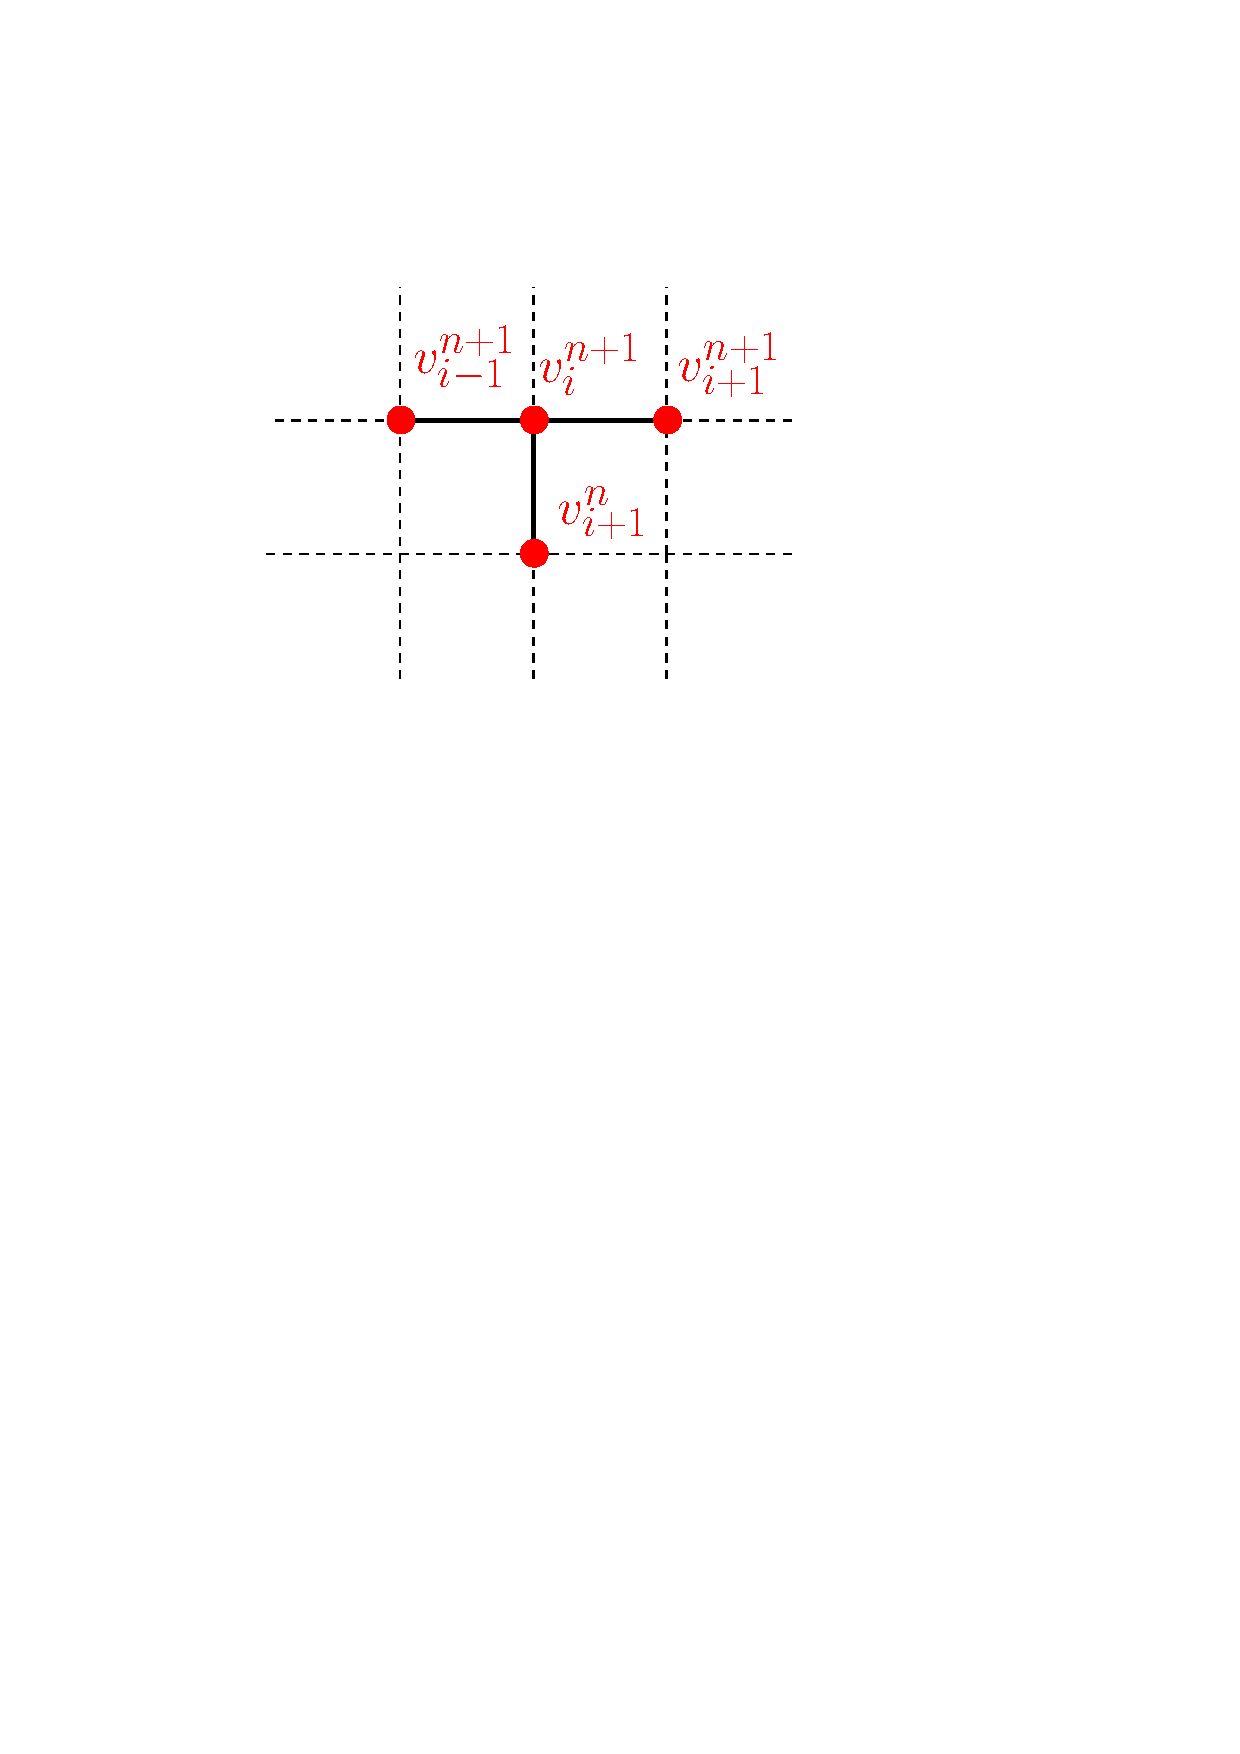
\includegraphics[scale=.8]{chapters/chapter3/ExplicitStencil.pdf}
  \caption{Stencil diagram of the explicit scheme.}
  \label{fig:finitedifferencesschemes:explicit_stencil}
\end{figure}
As it can be observed in figure \eqref{fig:finitedifferencesschemes:explicit_stencil}, the first and second order central finite difference approximations at node $(x_i, t_{n+1})$ require to compute the difference at the nodes $(x_{i-1}, t_{n+1})$ and $(x_{i+1}, t_{n+1})$. Hence, we can only approximate the spatial partial derivative at the internal region of the grid $\mathcal{G}$ given by the nodes $(x_i, t_n)$ for $i=1,\dots,M$. Also note, that the central finite difference has second order convergence in space. In other words, as we decrease $\Delta{x}$ by one decimal place, the approximation error will decrease by two decimal places. Analogously, the backward difference approximation at $t_{n+1}$ for $v(x, t)$ and the optimal exercise price $\bar{S}(t)$ is given by
\begin{align}
  \label{eq:finitedifferencesschemes:explicit:temporal_backward_finite_difference}
  \dfrac{v^{n+1}_{i} - v^{n}_{i}}{\Delta{t}} &= \dfrac{\partial{v}}{\partial{t}}+ O(\Delta{t}) \qquad & \text{for $n = N,\dots,0$ } \\
  \label{eq:finitedifferencesschemes:explicit:front_temporal_backward_finite_difference}
  \dfrac{\bar{S}^{n+1}-\bar{S}^{n}}{\Delta t} &= \bar{S}'(t) + O(\Delta{t}) \qquad & \text{for $n = N,\dots,0$ }
\end{align}
Contrary to the central finite difference, the backward finite difference approximations have first order convergence in time. While it would be desirable to have second order convergence for the temporal partial derivative approximation, it is not possible use central finite difference because we would be required to have two boundary conditions in the time axis. By combining the finite difference approximations \eqref{eq:finitedifferencesschemes:overview:first_order_central_difference}, \eqref{eq:finitedifferencesschemes:overview:second_order_central_difference}, \eqref{eq:finitedifferencesschemes:explicit:temporal_backward_finite_difference}, and \eqref{eq:finitedifferencesschemes:explicit:temporal_backward_finite_difference},the approximation of the PDE in \eqref{eq:blackscholes:frontfixingmethod:nielsen:american_options_bs_pde} is given by 
\begin{equation*}
  \begin{split}
    \dfrac{v^{n+1}_{i} - v^{n}_{i}}{\Delta{t}} & + \dfrac{1}{2}\sigma^2 x_i^2 \dfrac{v^{n+1}_{i-1} - 2v^{n+1}_{i} + v^{n+1}_{i+1}}{(\Delta{x})^2} \\ 
     & + x_i\bigg( (r-\delta) - \dfrac{1}{\bar{S}^{n+1}}\dfrac{\bar{S}^{n+1} - \bar{S}^{n}}{\Delta{t}} \bigg)\dfrac{v^{n+1}_{i+1} - v^{n+1}_{i-1}}{2\Delta{x}} - rv^{n+1}_{i} = 0
  \end{split}
\end{equation*}
for $i = 1, \dots, M$ and $n = N, \dots, 0$. To simplify the expression above, we introduce the terms 
\begin{align*}
  \lambda &:= \dfrac{\Delta{t}}{(\Delta{x})^2} \\
  A_i &:= \dfrac{\lambda}{2}\sigma^2x^{2}_i - \dfrac{\lambda}{2}\bigg((r-\delta) - \dfrac{1}{\Delta{t}}\bigg)x_i\Delta{x} & \text{for $i = 1, \dots, M$} \\ 
  B_i &:= 1 - \lambda\sigma^2x_i^2 - r\Delta{t} & \text{for $i = 1, \dots, M$} \\
  C_i &:= \dfrac{\lambda}{2}\sigma^2x^{2}_i + \dfrac{\lambda}{2}\bigg((r-\delta) - \dfrac{1}{\Delta{t}}\bigg)x_i\Delta{x} &  \text{for $i = 1, \dots, M$} \\
  D^{n+1}_{i} &:= \dfrac{x_i}{2\Delta{x}}\dfrac{v^{n+1}_{i+1} - v^{n+1}_{i-1}}{\bar{S}^{n+1}} &  \text{for $i = 1, \dots, M$}
\end{align*}
Then, we rearrange the finite difference approximation of the PDE as 
\begin{equation}
  v^{n}_{i} - D^{n+1}_{i}\bar{S}^n = A_i v^{n+1}_{i-1} + B_{i}v^{n+1}_{i} + C_{i}v^{n+1}_{i+1}
  \label{eq:finitedifferencesschemes:explicit:pde_simplified}
\end{equation}
for $i = 1, \dots, M$ and $t = N, \dots, 0$. Moreover, the PDE problem in \eqref{eq:blackscholes:frontfixingmethod:nielsen:american_options_bs_pde} have well-defined spatial boundary conditions. Remember that for call options, the boundary conditions are located at $x=0$ and $x=1$. Similarly, for put options, the boundary conditions are located at $x=1$ and at a sufficient large $x$. However, since the $\mathcal{G}$ is defined in terms of $x_\text{min}$ and $x_\text{max}$, regardless of the option type, the boundary conditions will be always at $x_0$ and $x_{M+1}$.
\begin{subequations}
  \label{eq:finitedifferencesschemes:explicit:boundary_conditions}
  \begin{align}
    \text{\textbf{Call:}} \qquad & v^{n}_{0} = 0, \qquad v^{n}_{M+1} = \bar{S}^{n} - K\\
    \text{\textbf{Put:}} \qquad & v^{n}_{0} = K - \bar{S}^{n}, \qquad v^{n}_{M+1} = 0
  \end{align}
\end{subequations}
Likewise, the terminal conditions are located at $t_{N+1}$ $i=0,\dots,M+1$
\begin{subequations}
  \label{eq:finitedifferencesschemes:explicit:terminal_conditions}
  \begin{equation}
    v^{N+1}_{i} = 0, \qquad \bar{S}^{N+1} = K
  \end{equation}
\end{subequations}
Moreover, for the problem \eqref{eq:blackscholes:frontfixingmethod:nielsen:american_options_bs_pde}, we have contact point condition \eqref{eq:blackscholes:frontfixingmethod:nielsen:american_options_optimal_price_contact_point_condition}. The contact point condition gives the slope at $x=1$. When the option is a call option, $x=1$ correspond to $x_{M+1}$ in the grid $\mathcal{G}$. Reciprocally, for a put option, $x=1$ correspond to $x_0$. Therefore, by using backward difference at $x_{M+1}$ and forward difference at $x_0$, the contact point approximation for call and put options, respectively.
\begin{align*}
  \text{\textbf{Call:}} \qquad & \dfrac{v^{n}_{M+1} - v^{n}_{M}}{\Delta{x}} = \dfrac{\partial{v}}{\partial{x}}(1, t) + O(\Delta{x}) \\
  \text{\textbf{Put:}} \qquad & \dfrac{v^{n}_{1} - v^{n}_{0}}{\Delta{x}} = \dfrac{\partial{v}}{\partial{x}}(1, t)+ O(\Delta{x}) 
\end{align*}
Using the contact point condition, we obtain an explicit expression for $v^{n}_{M}$
\begin{subequations}
  \label{eq:finitedifferencesschemes:explicit:contact_point_approximation_2}
  \begin{align}
    \text{\textbf{Call:}} \qquad& v^{n}_{M} = v^{n}_{M+1} - \Delta{x}\bar{S}^{n} = (1-\Delta{x})\bar{S}^n - K & \qquad \text{for $n = N,\dots,0$ }\\
    \text{\textbf{Put:}} \qquad& v^{n}_{1} = v^{n}_{0} - \Delta{x}\bar{S}^{n} = K - (1+\Delta{x})\bar{S}^n & \qquad \text{for $n = N,\dots,0$ }
  \end{align}    
\end{subequations}
Note that the approximation for $v^{n}_{M}$ has first order convergence in space which could degrade the global convergence of the explicit method to first order in space even if we are using central finite difference to approximate the spatial partial derivatives of $v(x,t)$. Similarly, we can obtain explicit expression for $\bar{S}^{n}$ by computing \eqref{eq:finitedifferencesschemes:explicit:pde_simplified} at $x_M$ and at $x_1$ for call and put options, respectively. Then, rearranging the resulting expression in terms of $\bar{S}^n$ 
\begin{subequations}
  \label{eq:finitedifferencesschemes:explicit:optimal_exercise_price_approximation}
  \begin{align}
    \text{\textbf{Call:}} \qquad& \bar{S}^{n} = \dfrac{K + A_{M}v^{n+1}_{M-1} + B_{M}v^{n+1}_{M} + C_{M}v^{n+1}_{M+1}}{(1-\Delta{x}) - D^{n+1}_{M}} \\
    \text{\textbf{Put:}} \qquad& \bar{S}^{n} = \dfrac{K - (A_{1}v^{n+1}_{0} + B_{1}v^{n+1}_{1} + C_{1}v^{n+1}_{2})}{D^{n+1}_1 + (1+\Delta{x})}
  \end{align}
\end{subequations}
for $n = N,\dots,0$. Thus, combining \eqref{eq:finitedifferencesschemes:explicit:pde_simplified}, \eqref{eq:finitedifferencesschemes:explicit:boundary_conditions}, 
\eqref{eq:finitedifferencesschemes:explicit:terminal_conditions},
\eqref{eq:finitedifferencesschemes:explicit:contact_point_approximation_2}, and \eqref{eq:finitedifferencesschemes:explicit:optimal_exercise_price_approximation}, the explicit scheme of PDE problem \eqref{eq:blackscholes:frontfixingmethod:nielsen:american_options_bs_pde} is given by
{
\allowdisplaybreaks
\begin{subequations}
\label{eq:finitedifferencesschemes:explicit:nielsen_system_of_equation}
\begin{align}
  \text{\textbf{Call:}} \quad& \begin{cases}
    v^{n}_{i} - D^{n+1}_{i}\bar{S}^n = A_i v^{n+1}_{i-1} + B_{i}v^{n+1}_{i} + C_{i}v^{n+1}_{i+1} & \text{for $i = 1, \dots, M-1$ and $n = N,\dots, 0$}\\
    v^{N+1}_i = 0 & \text{for $i = 0, \dots, M+1$}  \\
    \bar{S}^{N+1} = K \\
    v^{n}_0 = 0 & \text{for $n = N, \dots, 0$} \\ 
    v^{n}_{M} = (1-\Delta{x})\bar{S}^n - K & \text{for $n = N, \dots, 0$} \\
    v^{n}_{M+1} = \bar{S}^n - K  & \text{for $n = N, \dots, 0$}
  \end{cases}\\
  \text{\textbf{Put:}} \quad&  \begin{cases}
    v^{n}_{i} - D^{n+1}_{i}\bar{S}^n = A_i v^{n+1}_{i-1} + B_{i}v^{n+1}_{i} + C_{i}v^{n+1}_{i+1} & \text{for $i = 2, \dots, M$ and $n = N,\dots,0$} \\
    v^{N+1}_i = 0 & \text{for $i = 0, \dots, M+1$} \\ 
    \bar{S}^{N+1} = K \\
    v^{n}_{0} = K - \bar{S}^{n} & \text{for $n = N, \dots, 0$} \\
    v^{n}_{1} =  K - (1+\Delta{x})\bar{S}^{n}  & \text{for $n = N, \dots, 0$} \\
    v^{n}_{M} = 0 & \text{for $n = N, \dots 0$}
  \end{cases}
\end{align}
\end{subequations}
}
Finally, we formulate an algorithm for solving the system \eqref{eq:finitedifferencesschemes:explicit:nielsen_system_of_equation}
\begin{algorithm}[H]
  \caption{Explicit method for call options} \label{alg:finitedifferencesschemes:explicit:call_explicit_method_algorithm}
  \begin{algorithmic}[1]
  \Ensure $\lambda \le 0.5$
  
  \For{$i = 0,\dots,M+1$} 
    \State $v^{N+1}_i = 0 $
  \EndFor
  
  \State $\bar{S}^{N+1} = K$

  \For{$i = 1,\dots,M$} 
    \State $A_i = \dfrac{\lambda}{2}\sigma^2x^{2}_i - \dfrac{\lambda}{2}\bigg((r-\delta) - \dfrac{1}{\Delta{t}}\bigg)x_i\Delta{x}$
    \State $B_i = 1 - \lambda\sigma^2x_i^2 - r\Delta{t} $
    \State $C_i = \dfrac{\lambda}{2}\sigma^2x^{2}_i + \dfrac{\lambda}{2}\bigg((r-\delta) - \dfrac{1}{\Delta{t}}\bigg)x_i\Delta{x} $
  \EndFor
  
  \For{$n = N, \dots, 0$}
    \For{$i = 1, \dots, M$}
      \State $D^{n+1}_i = \dfrac{x_i}{2\Delta{x}}\dfrac{v^{n+1}_{i+1} - v^{n+1}_{i-1}}{\bar{S}^{n+1}}$
    \EndFor
    \State $\bar{S}^n = \dfrac{K + A_{M}v^{n+1}_{M-1} + B_{M}v^{n+1}_{M} + C_{M}v^{n+1}_{M+1}}{(1-\Delta{x}) - D^{n+1}_{M}}$
    \State $v^{n}_{0} = 0$
    \State $v^{n}_{M} = (1-\Delta{x})\bar{S}^{n} - K$
    \State $v^{n}_{M+1} = \bar{S}^{n} - K$
    \For{$i = 1, \dots, M-1$}
      \State $v^{n}_{i} = A_i v^{n+1}_{i-1} + B_{i}v^{n+1}_{i} + C_{i}v^{n+1}_{i+1} + D^{n+1}_{i}\bar{S}^n$
    \EndFor
  \EndFor
\end{algorithmic}
\end{algorithm}

\begin{algorithm}[H]
  \caption{Explicit method for put options}\label{alg:finitedifferencesschemes:explicit:put_explicit_method_algorithm}
  \begin{algorithmic}[1]
  \For{$i = 0,\dots,M+1$} 
    \State $v^{N+1}_i = 0 $
  \EndFor
  \State $\bar{S}^{N+1} = K$
  \For{$i = 1,\dots,M$} 
    \State $A_i = \dfrac{\lambda}{2}\sigma^2x^{2}_i - \dfrac{\lambda}{2}\bigg((r-\delta) - \dfrac{1}{\Delta{t}}\bigg)x_i\Delta{x}$
    \State $B_i = 1 - \lambda\sigma^2x_i^2 - r\Delta{t} $
    \State $C_i = \dfrac{\lambda}{2}\sigma^2x^{2}_i + \dfrac{\lambda}{2}\bigg((r-\delta) - \dfrac{1}{\Delta{t}}\bigg)x_i\Delta{x} $
  \EndFor
  \For{$n = N, \dots, 0$}
    \For{$i = 1, \dots, M$}
      \State $D^{n+1}_i = \dfrac{x_i}{2\Delta{x}}\dfrac{v^{n+1}_{i+1} - v^{n+1}_{i-1}}{\bar{S}^{n+1}}$
    \EndFor
    \State $\bar{S}^n = \dfrac{K - (A_{1}v^{n+1}_{0} + B_{1}v^{n+1}_{1} + C_{1}v^{n+1}_{2})}{D^{n+1}_{1} + (1+\Delta{x})}$
    \State $v^{n}_{0} = K - \bar{S}^{n}$
    \State $v^{n}_{1} = K - (1+\Delta{x})\bar{S}^n$
    \State $v^{n}_{M+1} = 0$
    \For{$i = 2, \dots, M$}
      \State $v^{n}_{i} = A_i v^{n+1}_{i-1} + B_{i}v^{n+1}_{i} + C_{i}v^{n+1}_{i+1} + D^{n+1}_{i}\bar{S}^n$
    \EndFor
  \EndFor
\end{algorithmic}
\end{algorithm}
\subsection{Implicit scheme}
Analogously to the previous section, implicit methods approximate the temporal partial derivative using backward difference and the spatial partial derivative using a central difference at time $t_n$ and position $x_i$. Since the PDE in \eqref{eq:blackscholes:frontfixingmethod:nielsen:american_options_bs_pde} is written backward in time, we use a forward difference instead.
\begin{figure}[H]
  \centering
  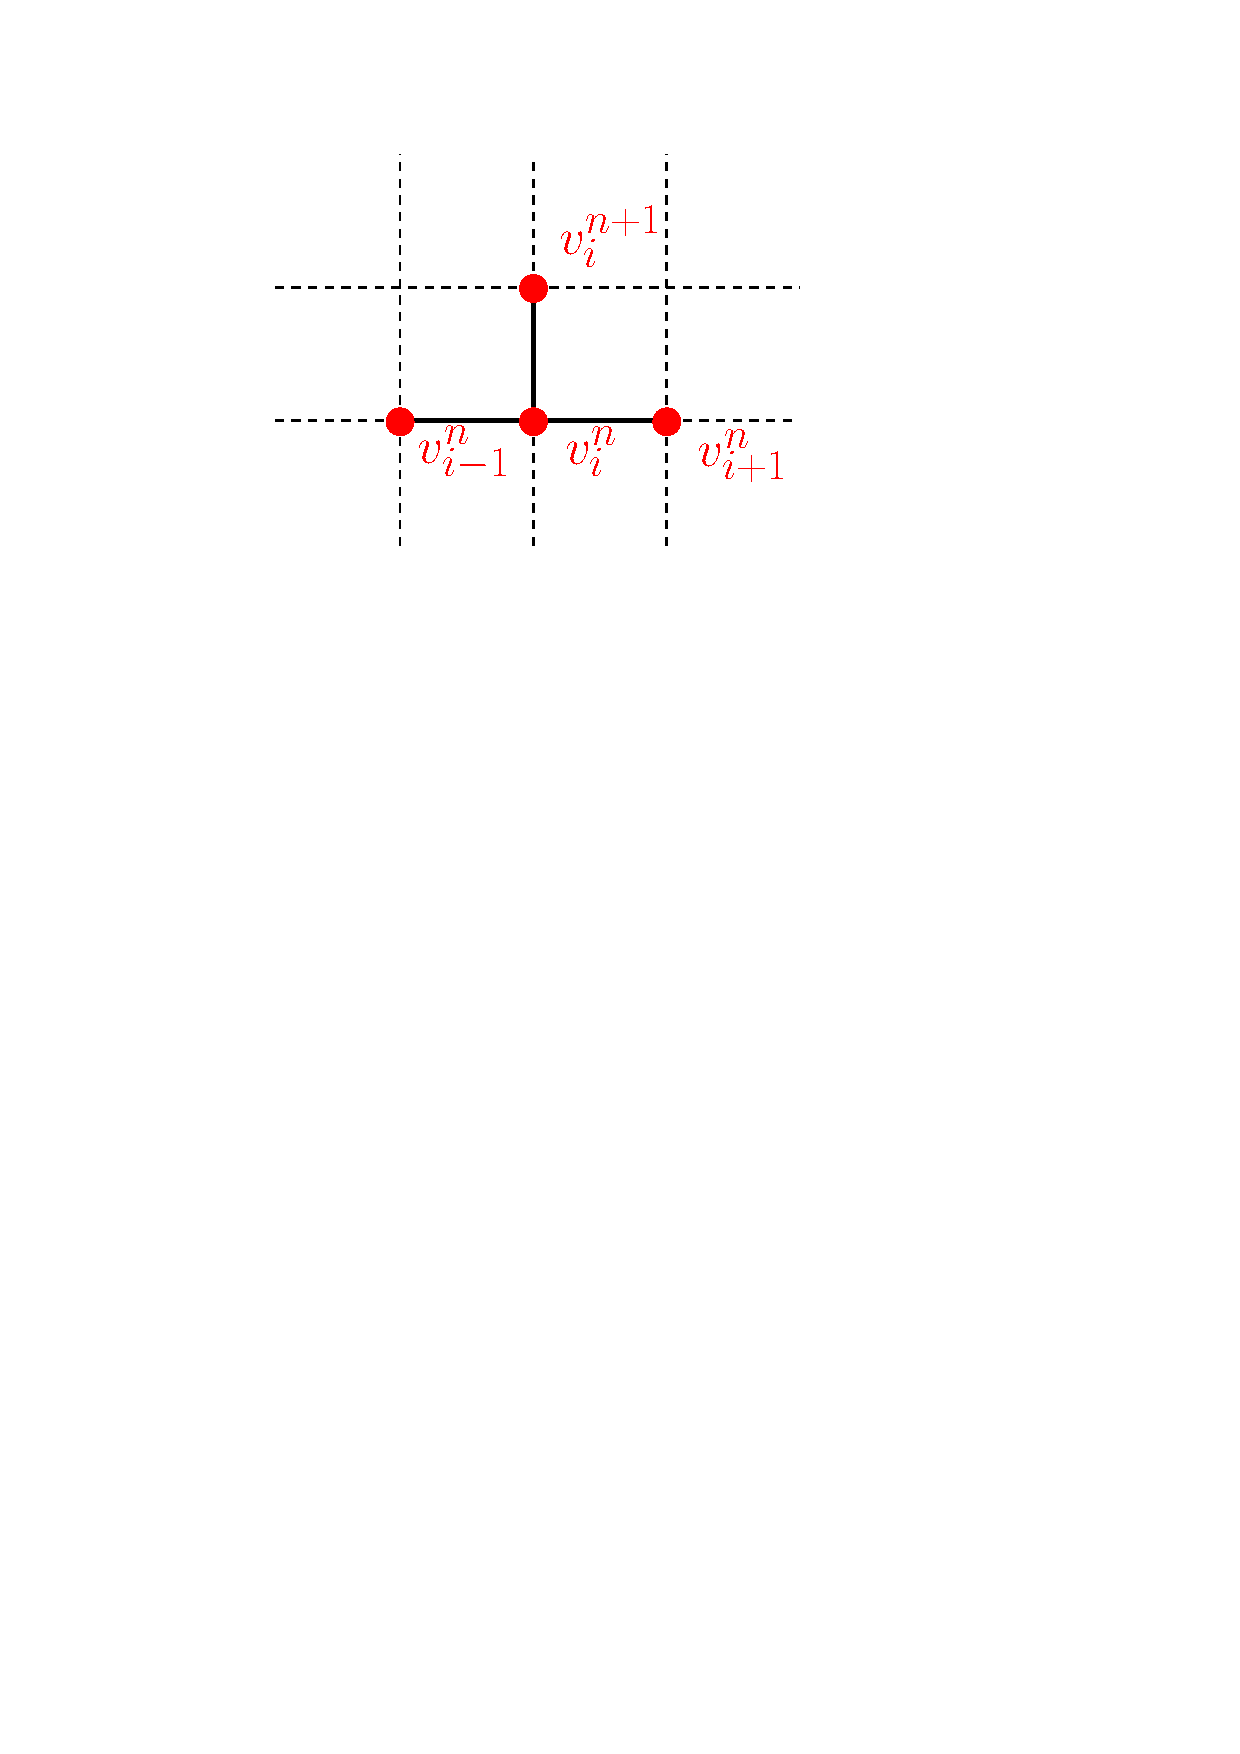
\includegraphics[scale=.8]{chapters/chapter3/ImplicitStencil.pdf}
  \caption{Stencil diagram of the implicit scheme.}
  \label{fig:finitedifferencesschemes:implicit_stencil}
\end{figure}
Therefore, the central difference for the first and second order spatial partial derivative at time $t_n$ is 
\begin{align}
  \label{eq:finitedifferencesschemes:implicit:spatial_first_order_central_finite_difference}
  \dfrac{v^{n}_{i+1} - v^{n}_{i-1}}{2 \Delta{x}} =& \dfrac{\partial{v}}{\partial{x}}+ O(\Delta{x}^2) \\
  \label{eq:finitedifferencesschemes:implicit:spatial_second_order_central_finite_difference}
  \dfrac{v^{n}_{i+1} - 2v^{n}_{i} + v^{n}_{i-1}}{\Delta{x}^2} =& \dfrac{\partial^2{v}}{\partial{x^2}}+ O(\Delta{x}^2)
\end{align}
for $i = 1, \dots, M$. Likewise, the forward difference of $v(x, t)$ and $\bar{S}(t)$ at position $x_i$ is  
\begin{align}
  \label{eq:finitedifferencesschemes:implicit:temporal_backward_finite_difference}
  \dfrac{v^{n+1}_{i} - v^{n}_{i}}{\Delta{t}} &= \dfrac{\partial{v}}{\partial{t}}+ O(\Delta{t}) \\
  \label{eq:finitedifferencesschemes:implicit:front_temporal_backward_finite_difference}
  \dfrac{\bar{S}^{n+1}-\bar{S}^{n}}{\Delta t} &= \bar{S}'(t) + O(\Delta{t}) \qquad & \text{ }
\end{align}
for $n = N,\dots,0$. Hence, combining \eqref{eq:finitedifferencesschemes:implicit:spatial_first_order_central_finite_difference}, \eqref{eq:finitedifferencesschemes:implicit:spatial_second_order_central_finite_difference}, \eqref{eq:finitedifferencesschemes:implicit:temporal_backward_finite_difference} and \eqref{eq:finitedifferencesschemes:implicit:front_temporal_backward_finite_difference},we obtain the implicit approximation of the PDE \eqref{eq:blackscholes:frontfixingmethod:nielsen:american_options_bs_pde} as
\begin{equation*}
  \begin{split}
    \dfrac{v^{n+1}_{i} - v^{n}_{i}}{\Delta{t}} & + \dfrac{1}{2}\sigma^2 x_i^2 \dfrac{v^{n}_{i-1} - 2v^{n}_{i} + v^{n}_{i+1}}{(\Delta{x})^2} \\ 
     & + x_i\bigg( (r-\delta) - \dfrac{1}{\bar{S}^{n}}\dfrac{\bar{S}^{n+1} - \bar{S}^{n}}{\Delta{t}} \bigg)\dfrac{v^{n}_{i+1} - v^{n}_{i-1}}{2\Delta{x}} - rv^{n}_{i} = 0
  \end{split}
\end{equation*}
for $i=1,\dots,M$ and $n=N,\dots,0$. Similar to the explicit method, the approximation error is second order in space and first order in time. Again, to make the implicit  approximation more manageable, we introduce the following terms  
\begin{align}
  \alpha^{n}_{i} &:= -\dfrac{\lambda}{2}\sigma^2x^{2}_{i} + \dfrac{\lambda\Delta{x}}{2}x_{i}\bigg(r-\delta+\dfrac{\bar{S}^{n+1}-\bar{S}^n}{\Delta{t}\bar{S}^{n}}\bigg) \\
  \beta^{n}_{i} &:= 1 + \lambda\sigma^2x^{2}_{i} + r\Delta{t} \\
  \gamma^{n}_{i} &:= -\dfrac{\lambda}{2}\sigma^2x^{2}_{i} + \dfrac{\lambda\Delta{x}}{2}x_{i}\bigg(r-\delta+\dfrac{\bar{S}^{n+1}-\bar{S}^n}{\Delta{t}\bar{S}^{n}}\bigg)
\end{align}
and rearrange the PDE as
\begin{equation}
  \label{eq:finitedifferencesschemes:implicit:implicit_scheme_simplified}
  \alpha^{n}_{i}v^{n}_{i-1} + \beta^{n}_{i}v^{n}_{i} + \gamma^{n}_{i}v^{n}_{i+1} = v^{n+1}_{i}
\end{equation}
The boundary and terminal conditions are given by \eqref{eq:finitedifferencesschemes:explicit:boundary_conditions} and \eqref{eq:finitedifferencesschemes:explicit:terminal_conditions}. Likewise, the approximation of $v^{n}_{M}$ or $v^{n}_{1}$ for put and call, respectively, is given by \eqref{eq:finitedifferencesschemes:explicit:contact_point_approximation_2}. Similar to the explicit method, the approximation $v^{n}_{M}$ and $v^{n}_{0}$ given by the contact point condition is first order in space. Hence, the global approximation error of implicit scheme might be degraded to first order in space. Contrary to the explicit method, there is not an explicit expression for $\bar{S^n}$. Now, we formulate the system of equations of the problem \eqref{eq:blackscholes:frontfixingmethod:nielsen:american_options_bs_pde}
using \eqref{eq:finitedifferencesschemes:explicit:boundary_conditions}, \eqref{eq:finitedifferencesschemes:explicit:terminal_conditions}, \eqref{eq:finitedifferencesschemes:explicit:contact_point_approximation_2} and \eqref{eq:finitedifferencesschemes:implicit:implicit_scheme_simplified}
{
  \allowdisplaybreaks
  \begin{subequations}
  \label{eq:finitedifferencesschemes:implicit:nielsen_system_of_equation}
  \begin{align}
    \text{\textbf{Call:}} \quad& \begin{cases}
      \alpha^{n}_{i}v^{n}_{i-1} + \beta^{n}_{i}v^{n}_{i} + \gamma^{n}_{i}v^{n}_{i+1} = v^{n+1}_{i} & \text{for $i = 1, \dots, M-1$ and $n = N,\dots,0$} \\
      v^{N+1}_i = 0 & \text{for $i = 0, \dots, M+1$}\\
      \bar{S}^{N+1} = K \\
      v^{n}_0 = 0 & \text{for $n = N, \dots 0$}\\
      v^{n}_{M} = (1-\Delta{x})\bar{S}^n - K & \text{for $n = N, \dots 0$}\\
      v^{n}_{M+1} = \bar{S}^n - K  & \text{for $n = N, \dots 0$}
    \end{cases}\\
    \text{\textbf{Put:}} \quad& \begin{cases}
      \alpha^{n}_{i}v^{n}_{i-1} + \beta^{n}_{i}v^{n}_{i} + \gamma^{n}_{i}v^{n}_{i+1} = v^{n+1}_{i} & \text{for $i = 2, \dots, M$ and $n = N,\dots,0$} \\
      v^{N+1}_i = 0 & \text{for $i = 0, \dots, M+1$} \\
      \bar{S}^{N+1} = K \\
      v^{n}_{0} = K - \bar{S}^{n} & \text{for $n = N, \dots 0$}\\
      v^{n}_{1} =  K - (1+\Delta{x})\bar{S}^{n} & \text{for $n = N, \dots 0$}\\
      v^{n}_{M} = 0 & \text{for $n = N, \dots 0$}
    \end{cases}
  \end{align}
\end{subequations}
}
Note that the system of equation above is cannot be solved explicitly as we did for \eqref{eq:finitedifferencesschemes:explicit:nielsen_system_of_equation}. In normal circumstance, solving the system above would require to solve a system of linear equations consisting of $M-1$ unknowns (including $\bar{S}^{n}$). However, the terms $\alpha_i$ and $\gamma_i$ are a nonlinear with respect of $\bar{S}^{n}$ which indicate us that instead we will have to solve a system nonlinear of equations. Let us define the vector $\mathbf{v}^n \in \mathbb{R}^{M-2}$ as
\begin{subequations}
  \begin{align}
    \text{\textbf{Call:}} \qquad \mathbf{v}^{n} :=& \begin{bmatrix}
      v^{n}_{1}, & v^{n}_{2}, & \cdots, & v^{n}_{M-1}
    \end{bmatrix}^{\text{T}}\\
    \text{\textbf{Put:}} \qquad \mathbf{v}^{n} :=& \begin{bmatrix}
      v^{n}_{2}, & v^{n}_{3}, & \cdots, & v^{n}_{M}
    \end{bmatrix}^{\text{T}}
  \end{align}    
\end{subequations}
the matrix $\mathbf{\Lambda}^{n} \in \mathbb{R}^{M-1,M-2}$ 
{
  \allowdisplaybreaks  
\begin{subequations}
  \begin{align}
    \text{\textbf{Call:}} \qquad \mathbf{\Lambda}^{n} =& \begin{bmatrix}
      \beta^{n}_{1} & \gamma^{n}_1 \\
      \alpha^{n}_{2} & \beta^{n}_{2} & \gamma^{n}_{2} \\
      & \ddots & \ddots & \ddots  \\
      & & \ddots & \ddots & \ddots  \\
      & & & \alpha^{n}_{M-2} & \beta^{n}_{M-2} & \gamma^{n}_{M-2} \\
      & & & & \alpha^{n}_{M-1} & \beta^{n}_{M-1} \\
      & & & & & \alpha^{n}_{M} \\
    \end{bmatrix}\\
    \text{\textbf{Put:}} \qquad  \mathbf{\Lambda}^{n} :=& \begin{bmatrix}
      \gamma^{n}_1 \\
      \beta^{n}_2 & \gamma^{n}_2 \\
      \alpha^{n}_3 & \beta^{n}_3 & \gamma^{n}_3 \\
      & \ddots & \ddots & \ddots \\
      & & \ddots & \ddots & \ddots \\
      & & & \alpha^{n}_{M-1} & \beta^{n}_{M-1} & \gamma^{n}_{M-1} \\
      & & & & \alpha^{n}_{M} & \beta^{n}_{M} \\
    \end{bmatrix}
  \end{align}
\end{subequations}
}
and the vector $\mathbf{f}^{n} \in \mathbb{R}^{M-1}$
\begin{subequations}
  \begin{align}
    \text{\textbf{Call:}} \qquad \mathbf{f}^n :=& \begin{bmatrix}
      v^{n+1}_{1} \\
      \vdots \\
      v^{n+1}_{M-1} - \gamma^{n}_{M-1}[(1-\Delta{x})\bar{S}^{n} - K] \\
      v^{n+1}_{M} - \gamma^{n}_{M}(\bar{S}^n - K) - \beta^{n}_{M}[(1-\Delta{x})\bar{S}^{n} - K]
    \end{bmatrix}\\
    \text{\textbf{Put:}} \qquad \mathbf{f}^n :=& \begin{bmatrix}
      v^{n+1}_{1} - \alpha^{n}_{1}(K - \bar{S}^{n}) - \beta^{n}_{1}[K - (1+\Delta{x})\bar{S}^{n}] \\
      v^{n+1}_{2} - \beta^{n}_2[K - (1+\Delta{x})\bar{S}^{n}] \\
      v^{n+1}_{3} \\
      \vdots \\
      v^{n+1}_{M-1}
    \end{bmatrix}
  \end{align}
\end{subequations}
Thus, we have to solve the nonlinear system of equations
\begin{equation}
  \mathbf{F}\big(\begin{bmatrix}
    \mathbf{v}^{n} | \bar{S}^{n}
  \end{bmatrix}^{\text{T}}\big) = \Lambda^{n}\mathbf{v}^{n} - \mathbf{f}^n = 0
\end{equation}
We can use newton's method to solve the nonlinear system iteratively
\begin{equation}
  \mathbf{y}_{k+1} = \mathbf{y}_{k} - \mathbf{J}^{-1}(\mathbf{y}_{k})\mathbf{F}(\mathbf{y}_{k})
\end{equation}
where $\mathbf{J}(\mathbf{y}_k)\in\mathbb{R}^{(M-1)\times(M-1)}$ is the Jacobian of $\mathbf{F}(\mathbf{y}_k)$, $\mathbf{y}_k\in\mathbb{R}^{M-1}$ is some approximation of true solution
\begin{equation}
  \mathbf{y} = \begin{bmatrix}
    \mathbf{v}^{n} | \bar{S}^{n}
  \end{bmatrix}^{\text{T}}
\end{equation}
an initial value 
\begin{equation}
  \mathbf{y}_{0} = \begin{bmatrix}
    \mathbf{v}^{n+1} | \bar{S}^{n+1}
  \end{bmatrix}^{\text{T}}
\end{equation}

\subsection{Numerical results}
\subsubsection{Numerical experiments}
Generally, Datasets for American options are expensive to acquire. Therefore, to validate our implementation, we mainly relied on the data available in Company, 
et al.\cite*{company_egorova_jodar_2014}, Nielsen, et al.\cite*{nielsen_2001}, Seydel\cite*{seydel_2009}, and Wilmott, et al.\cite*{dewynne_howison_wilmott_howison_1995}. Moreover, used the approximations produced by binary option pricing model\cite{cox_1979} (BOPM)  as benchmark for assessing the consistency of our method. We chose the binomial model because it is widely used in the industry, and is simple to implement. Moreover, the BOPM uses a completely different approach to price options than the one considered in this dissertation. The first experiment that come into mind is to price call and put options without dividend. Therefore, let us define the parameter for the numerical experiment as
\begin{equation}
  \label{eq:numericaresults:parameters_set_1}
  K = 1, \quad T = 1, \quad r=0.2, \quad \sigma=0.02, \quad \delta = 0 
\end{equation}
from Nielsen et al.\cite{nielsen_2001}, we know that this set of parameters produce the optimal exercise boundary $\bar{S}(t) \approx 0.86$. Also, we approximated $\bar{S}(t)$ using the binomial option pricing model. Finally, we priced call and put options using the explicit  \eqref{eq:finitedifferencesschemes:explicit:nielsen_system_of_equation} and implicit \eqref{eq:finitedifferencesschemes:implicit:nielsen_system_of_equation} front fixing schemes based Nielsen transformation, and the explicit front fixing scheme based on the Company transformation \eqref{alg:appendix:companytransformation:explicits:put_explicit_method_algorithm} (See appendix). As you can observe in figure \eqref{fig:finitedifferencesschemes:numericaresults:test_case_1_explicit_company},
\eqref{fig:finitedifferencesschemes:numericaresults:test_case_1_explicit_nielsen}, and \eqref{fig:finitedifferencesschemes:numericaresults:test_case_1_implicit_nielsen},
both the Nielsen and Company schemes do not produce the value function as per figure \eqref{fig:blackscholes:preliminaries:american_call_value_vs_curve}. However, by taking a look to figure \eqref{fig:finitedifferencesschemes:numericaresults:test_case_1_bopm}, you can observe that the binomial option pricing model is also not capturing the geometrical properties described by figure \eqref{fig:blackscholes:preliminaries:american_call_value_vs_curve}. In fact, Merton\cite{merton_1973} showed that, pricing American options without dividends is equivalent to solve \eqref{eq:chapter2:european_option_pde_with_dividens} with boundary conditions $V(0, t)=0$ and $\lim_{S->\infty}V(S,t)=S-K$. Therefore, the problem reduces from a free boundary problem to a boundary problem. Thus, making the front fixing Nielsen and Company PDEs inappropriate for American call options without dividends.
\begin{figure}[tbp]
  \centering
  \begin{subfigure}{0.4\textwidth}
    \centering
    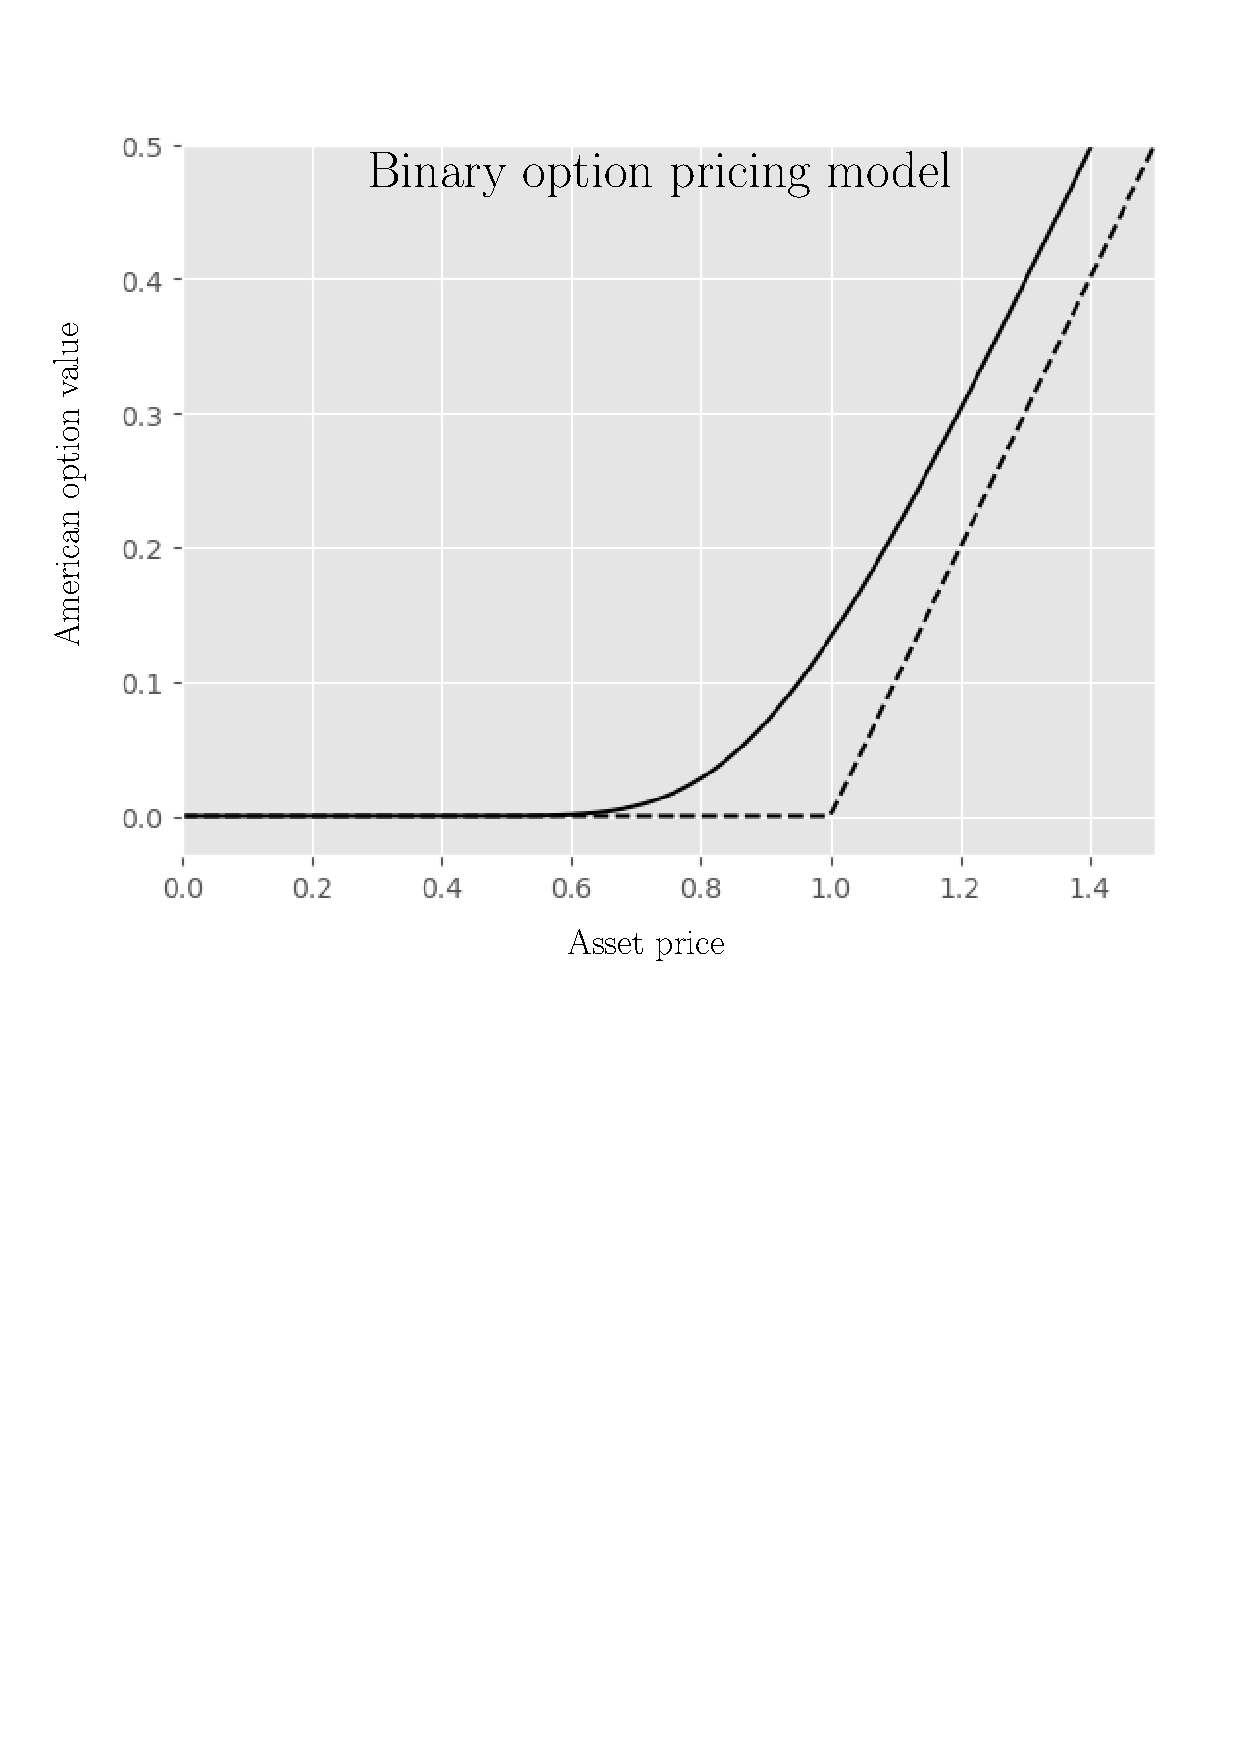
\includegraphics[width=\textwidth]{chapters/chapter3/TestCase1BOPM.pdf}
    \caption{$\text{Nodes} = 2^{500}$.}
    \label{fig:finitedifferencesschemes:numericaresults:test_case_1_bopm}
  \end{subfigure}
  \hspace{0.5cm}
  \begin{subfigure}{0.4\textwidth}
    \centering
    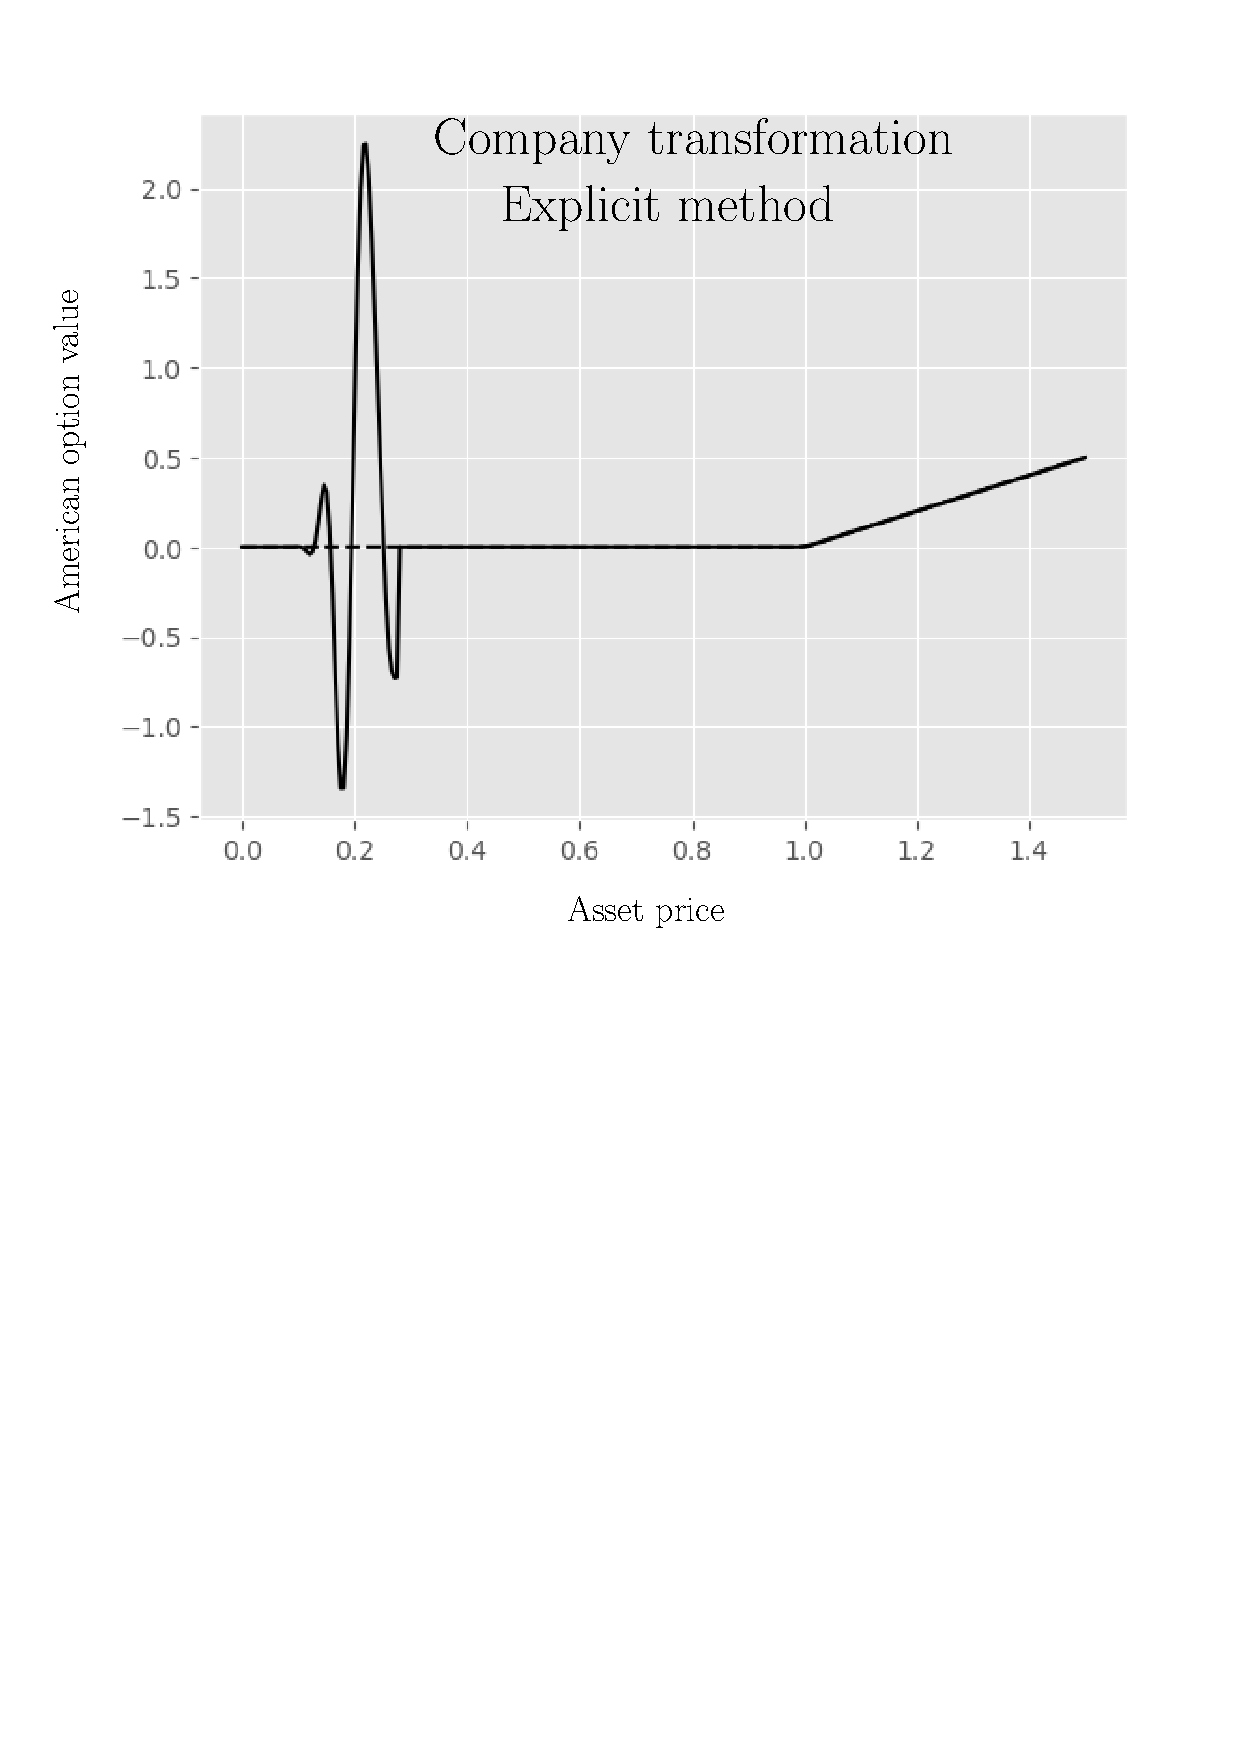
\includegraphics[width=\textwidth]{chapters/chapter3/TestCase1ExplicitCompany.pdf}
    \caption{$\Delta{x}=\expnumber{1}{-3}$ and $\Delta{t}=0.5\times\expnumber{1}{-6}$}
    \label{fig:finitedifferencesschemes:numericaresults:test_case_1_explicit_company}
  \end{subfigure}
  \begin{subfigure}{0.4\textwidth}
    \centering
    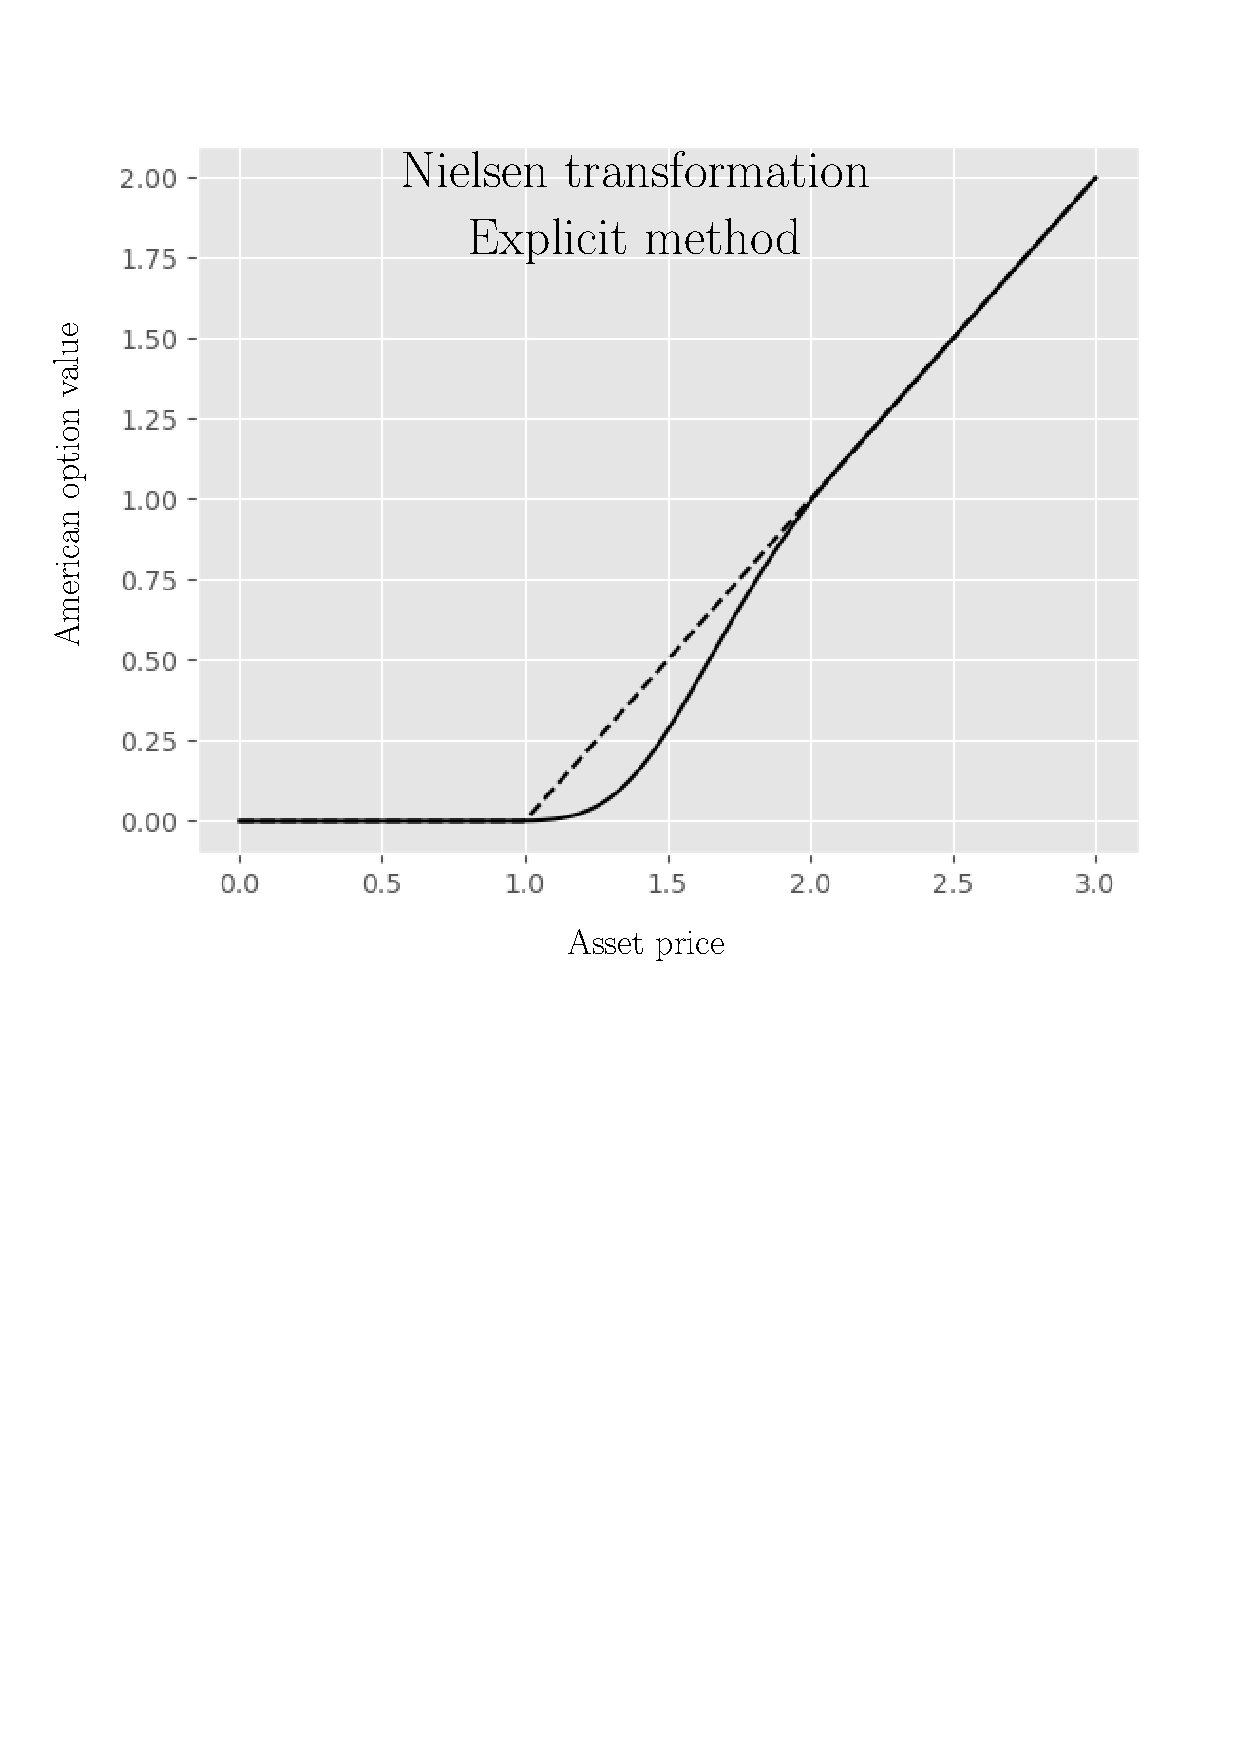
\includegraphics[width=\textwidth]{chapters/chapter3/TestCase1ExplicitNielsen.pdf}
    \caption{$\Delta{x}=\expnumber{1}{-3}, \Delta{t}=0.5\times\expnumber{1}{-6}$}
    \label{fig:finitedifferencesschemes:numericaresults:test_case_1_explicit_nielsen}
  \end{subfigure}
  \hspace{0.5cm}
  \begin{subfigure}{0.4\textwidth}
    \centering
    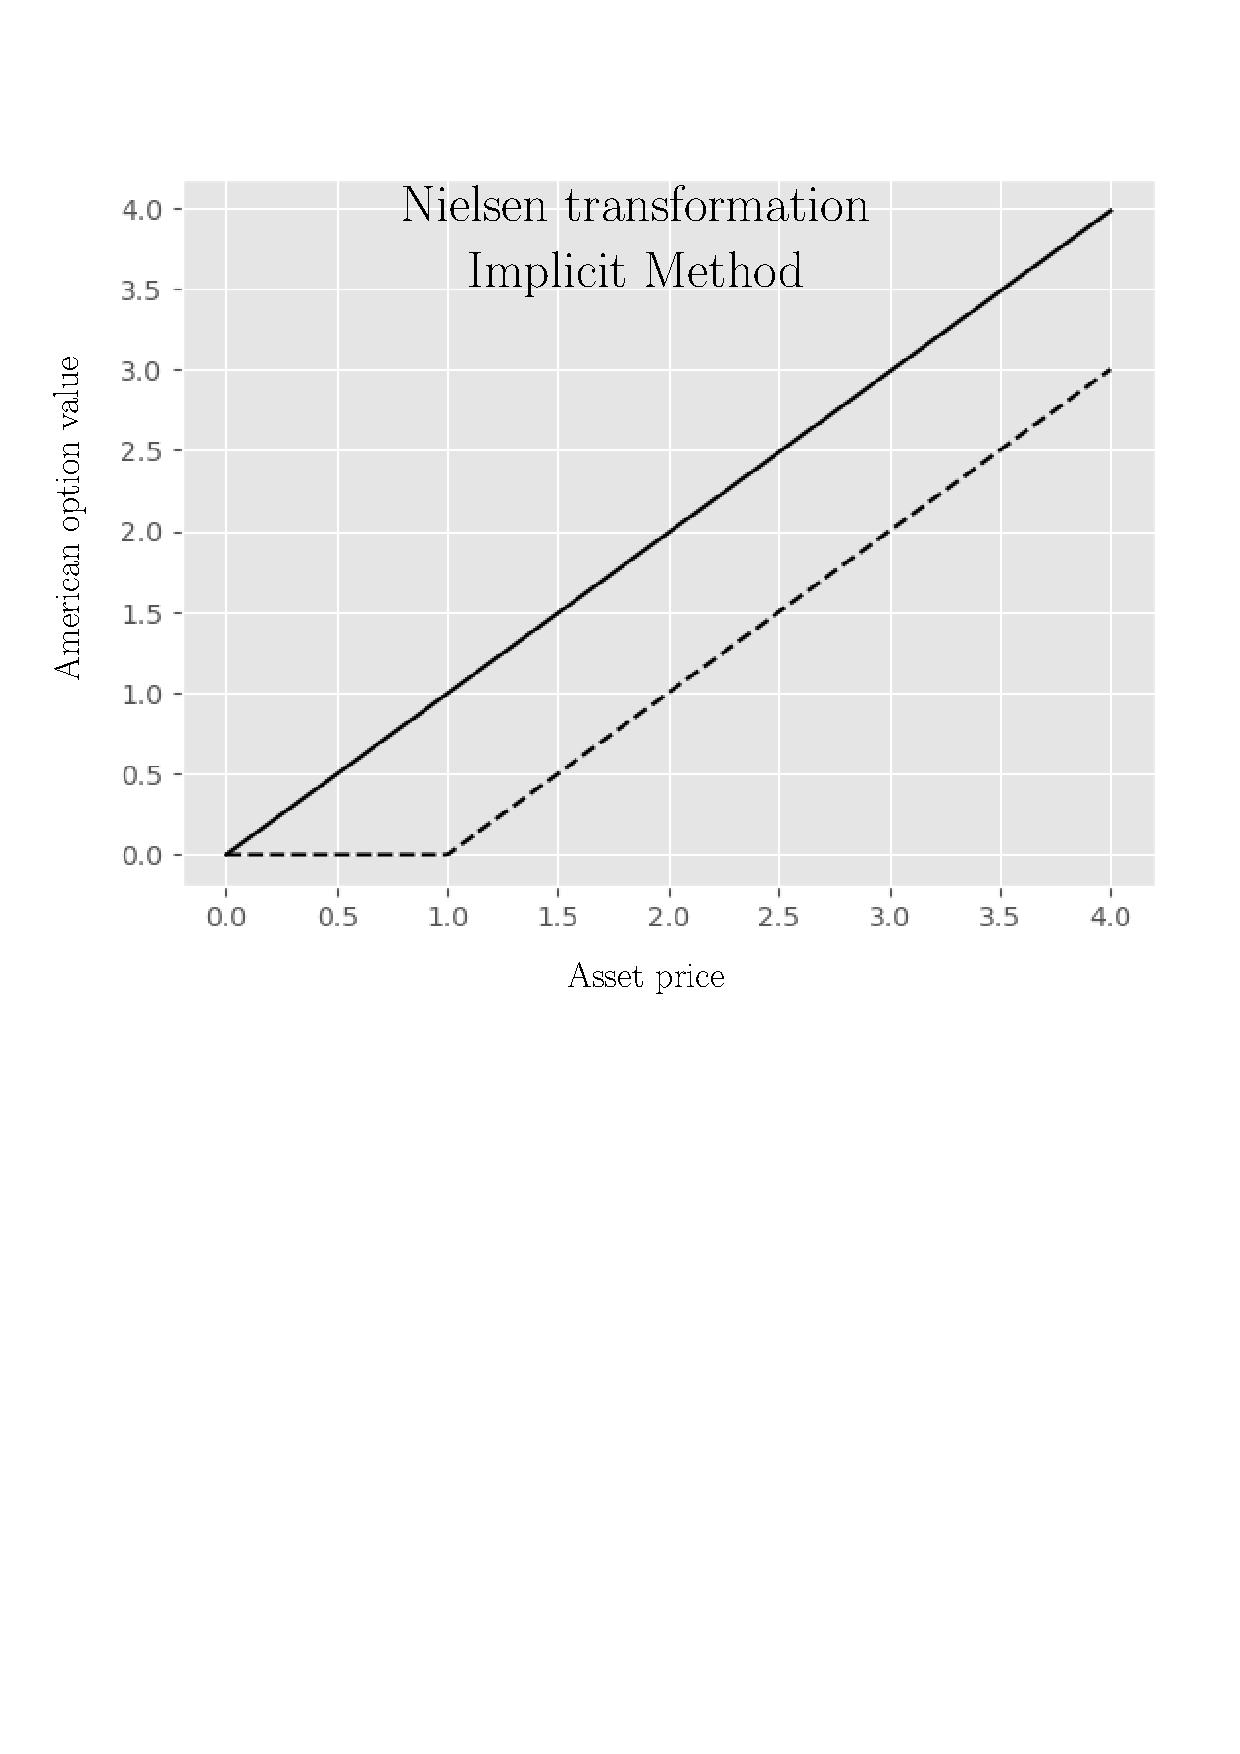
\includegraphics[width=\textwidth]{chapters/chapter3/TestCase1ImplicitNielsen.pdf}
    \caption{$\Delta{x}=\expnumber{1}{-3}, \Delta{t}=0.5\times\expnumber{1}{-6}$}
    \label{fig:finitedifferencesschemes:numericaresults:test_case_1_implicit_nielsen}
  \end{subfigure}
  \caption{American call option value $V(S, 0)$ given parameters \eqref{eq:numericaresults:parameters_set_1}.}
  \label{fig:finitedifferencesschemes:numericaresults:test_case_1_explicit}
\end{figure}

Now, let us consider the case of pricing put options without dividends given parameters \eqref{eq:numericaresults:parameters_set_1}. Figures \eqref{fig:finitedifferencesschemes:numericaresults:test_case_2} show the $V(S, 0)$ curve obtained by all the schemes. In each plot, we have listed the optimal exercise boundary $\bar{S}(0)$. Also, we have listed the corresponding value curve approximated using the binary option pricing model using $2^{500}$ nodes. As you see, Nielsen and Company approximated the optimal exercise boundary within 2 decimal places. Moreover, in table \eqref{tab:rsme_explicit_company_transformation_2}, we listed the approximation at several point along the value curve $V(S,t)$. Contrary to the case for call options, the value curves in \eqref{fig:finitedifferencesschemes:numericaresults:test_case_2} captured the geometry of American put options described by figure \eqref{fig:blackscholes:preliminaries:american_put_value_vs_curve}. Specifically, within the continuation region $S>\bar{S}(0)$, the value is larger than the payoff $V(S,0)>\max(K-S,0)$ and $V(S,0)\rightarrow0$ as $S\rightarrow0$. In addition, the value curve is exactly the payoff in the exercise region $S<\bar{S}(0)$. Finally, the explicit schemes yielded a significantly small RSME with a very low execution time. 
\begin{figure}[tbp]
  \centering
  \begin{subfigure}{0.4\textwidth}
    \centering
    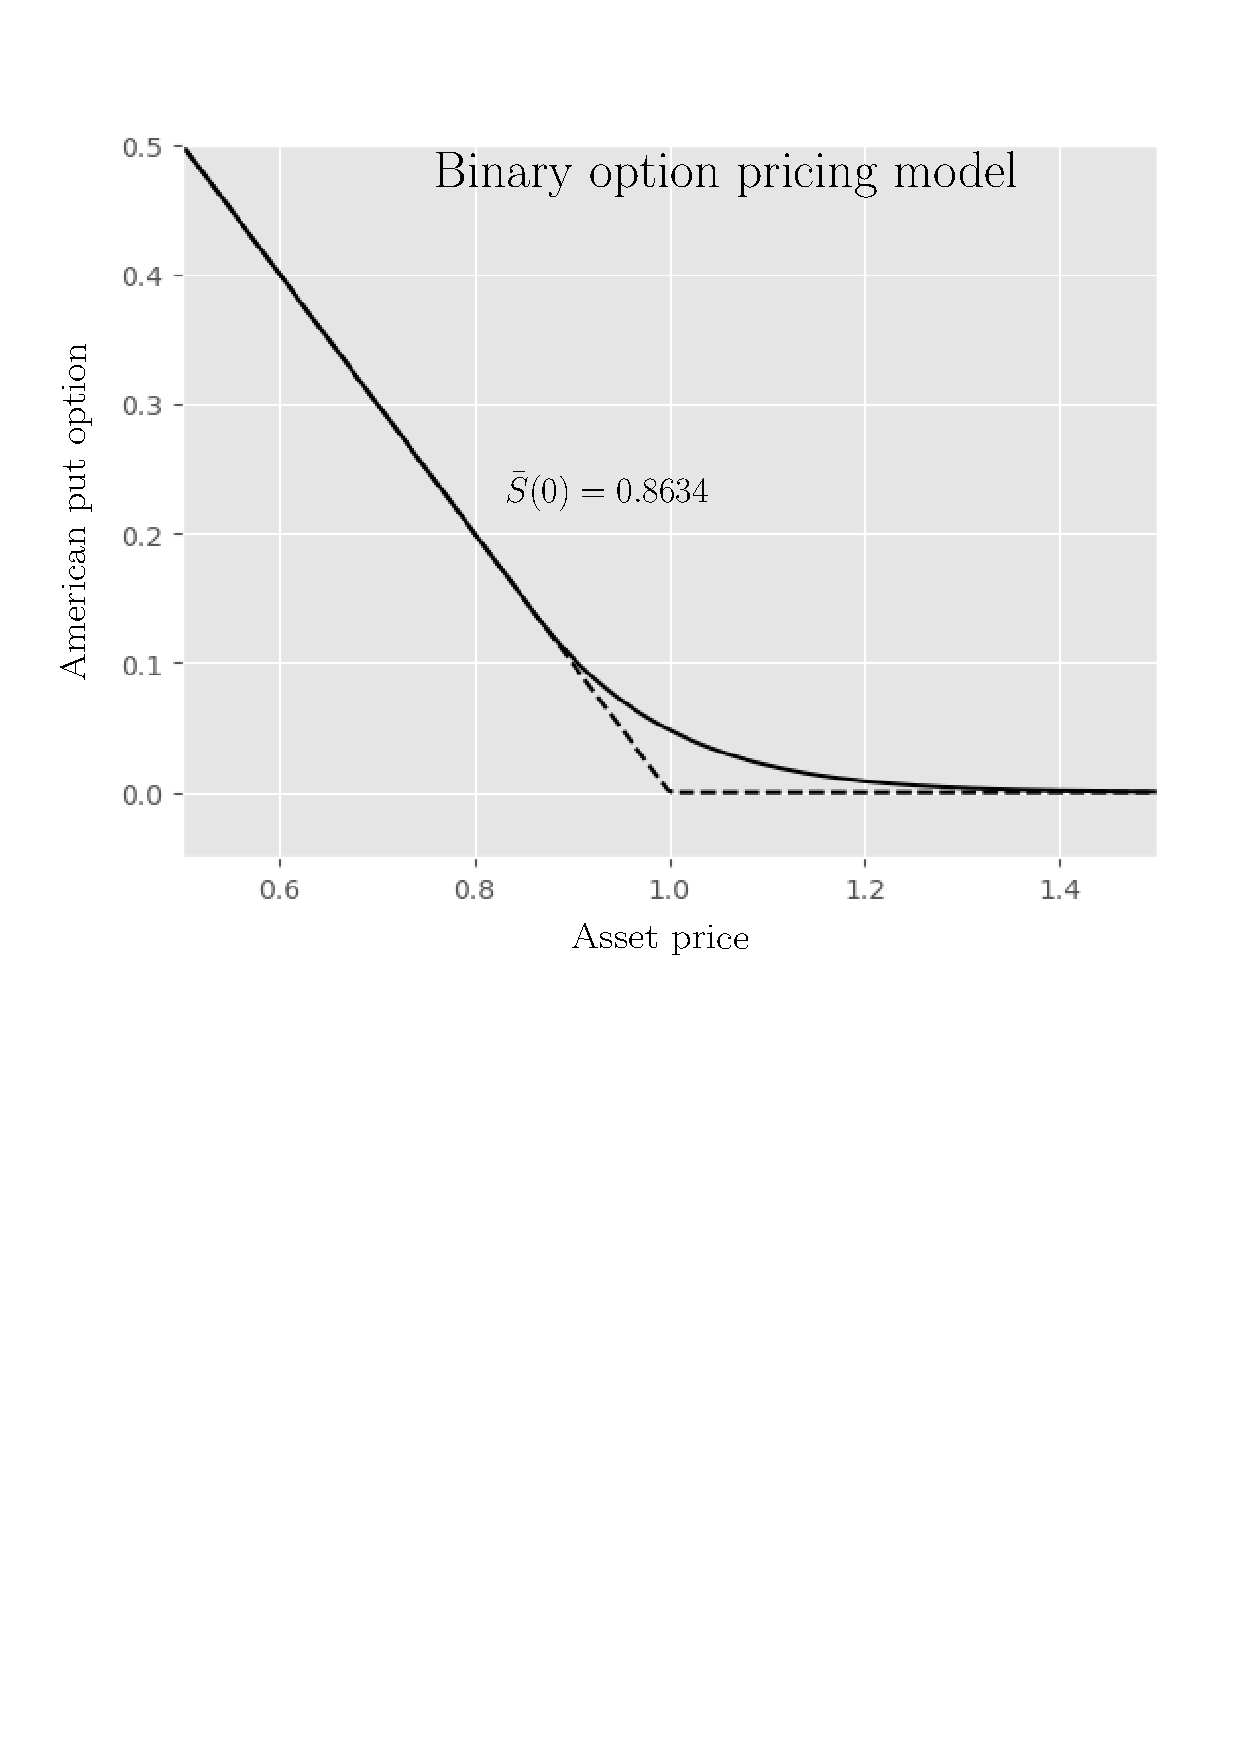
\includegraphics[width=\textwidth]{chapters/chapter3/TestCase2BOPM.pdf}
    \caption{$\text{Nodes} = 2^{500}$.}
    \label{fig:finitedifferencesschemes:numericaresults:test_case_2_bopm}
  \end{subfigure}
  \hspace{0.5cm}
  \begin{subfigure}{0.4\textwidth}
    \centering
    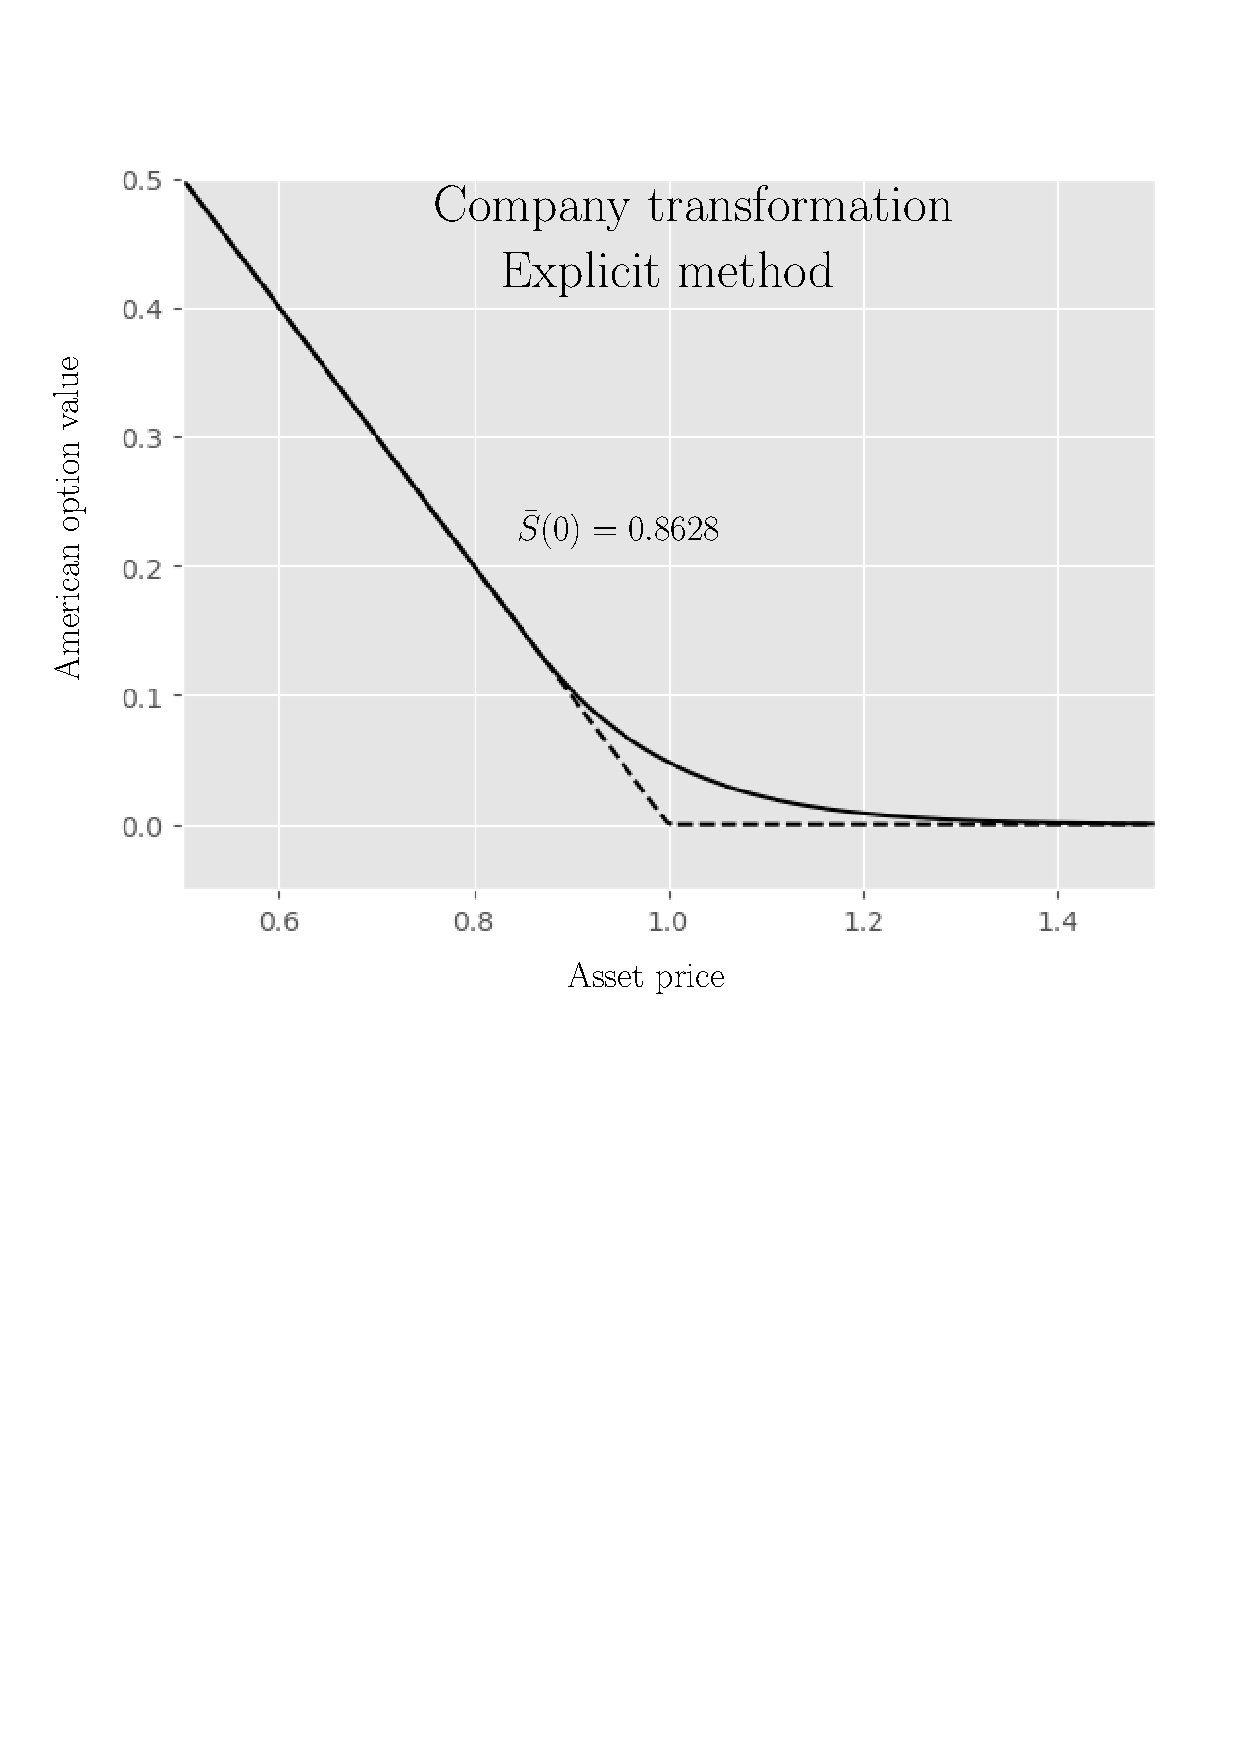
\includegraphics[width=\textwidth]{chapters/chapter3/TestCase2CompanyExplicit.pdf}
    \caption{$\Delta{x}=\expnumber{1}{-3}, \Delta{t}=0.5\times\expnumber{1}{-6}$}
    \label{fig:finitedifferencesschemes:numericaresults:test_case_2_explicit_company}
  \end{subfigure}
  \begin{subfigure}{0.4\textwidth}
    \centering
    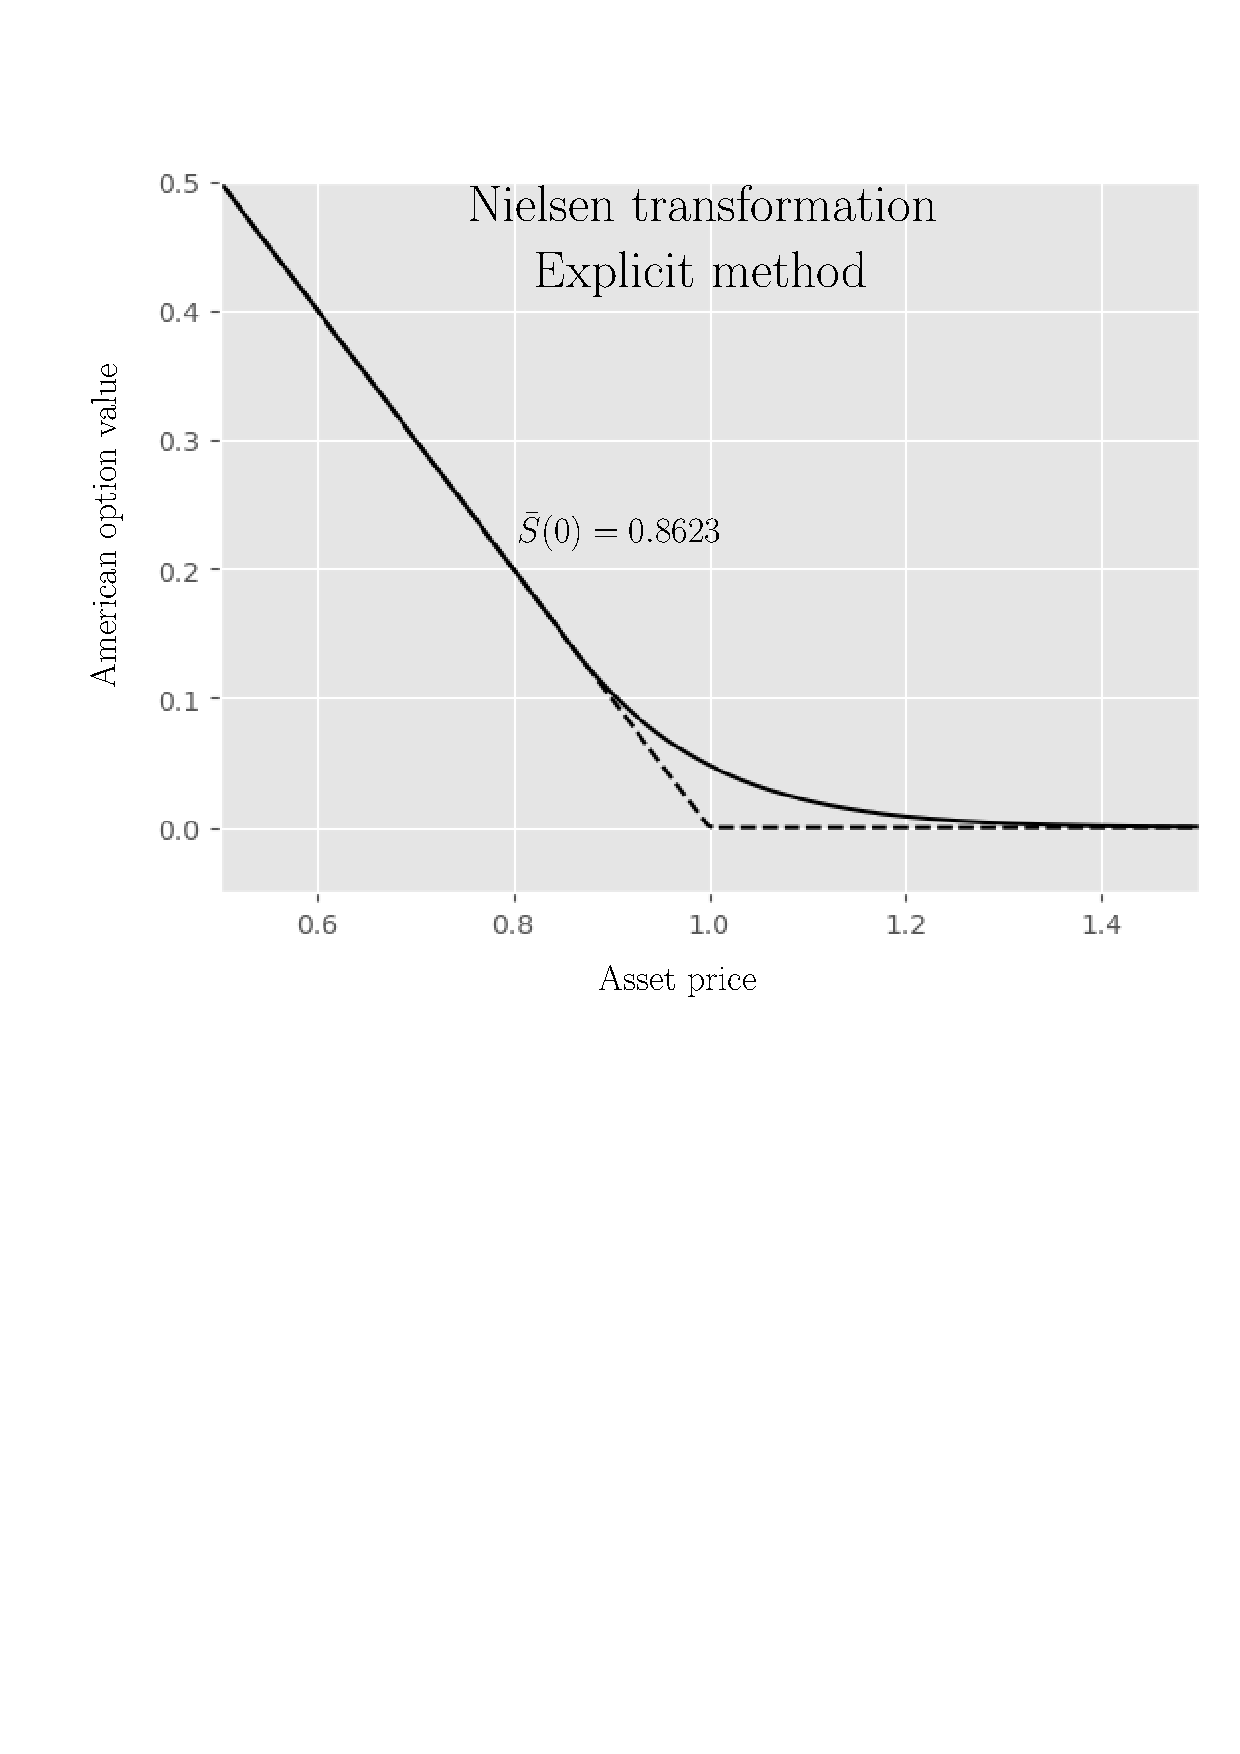
\includegraphics[width=\textwidth]{chapters/chapter3/TestCase2NielsenExplicit.pdf}
    \caption{$\Delta{x}=\expnumber{1}{-3}, \Delta{t}=0.5\times\expnumber{1}{-6}$}
    \label{fig:finitedifferencesschemes:numericaresults:test_case_2_explicit_nielsen}
  \end{subfigure}
  \hspace{0.5cm}
  \begin{subfigure}{0.4\textwidth}
    \label{fig:finitedifferencesschemes:numericaresults:test_case_2_implicit_nielsen}
    \centering
    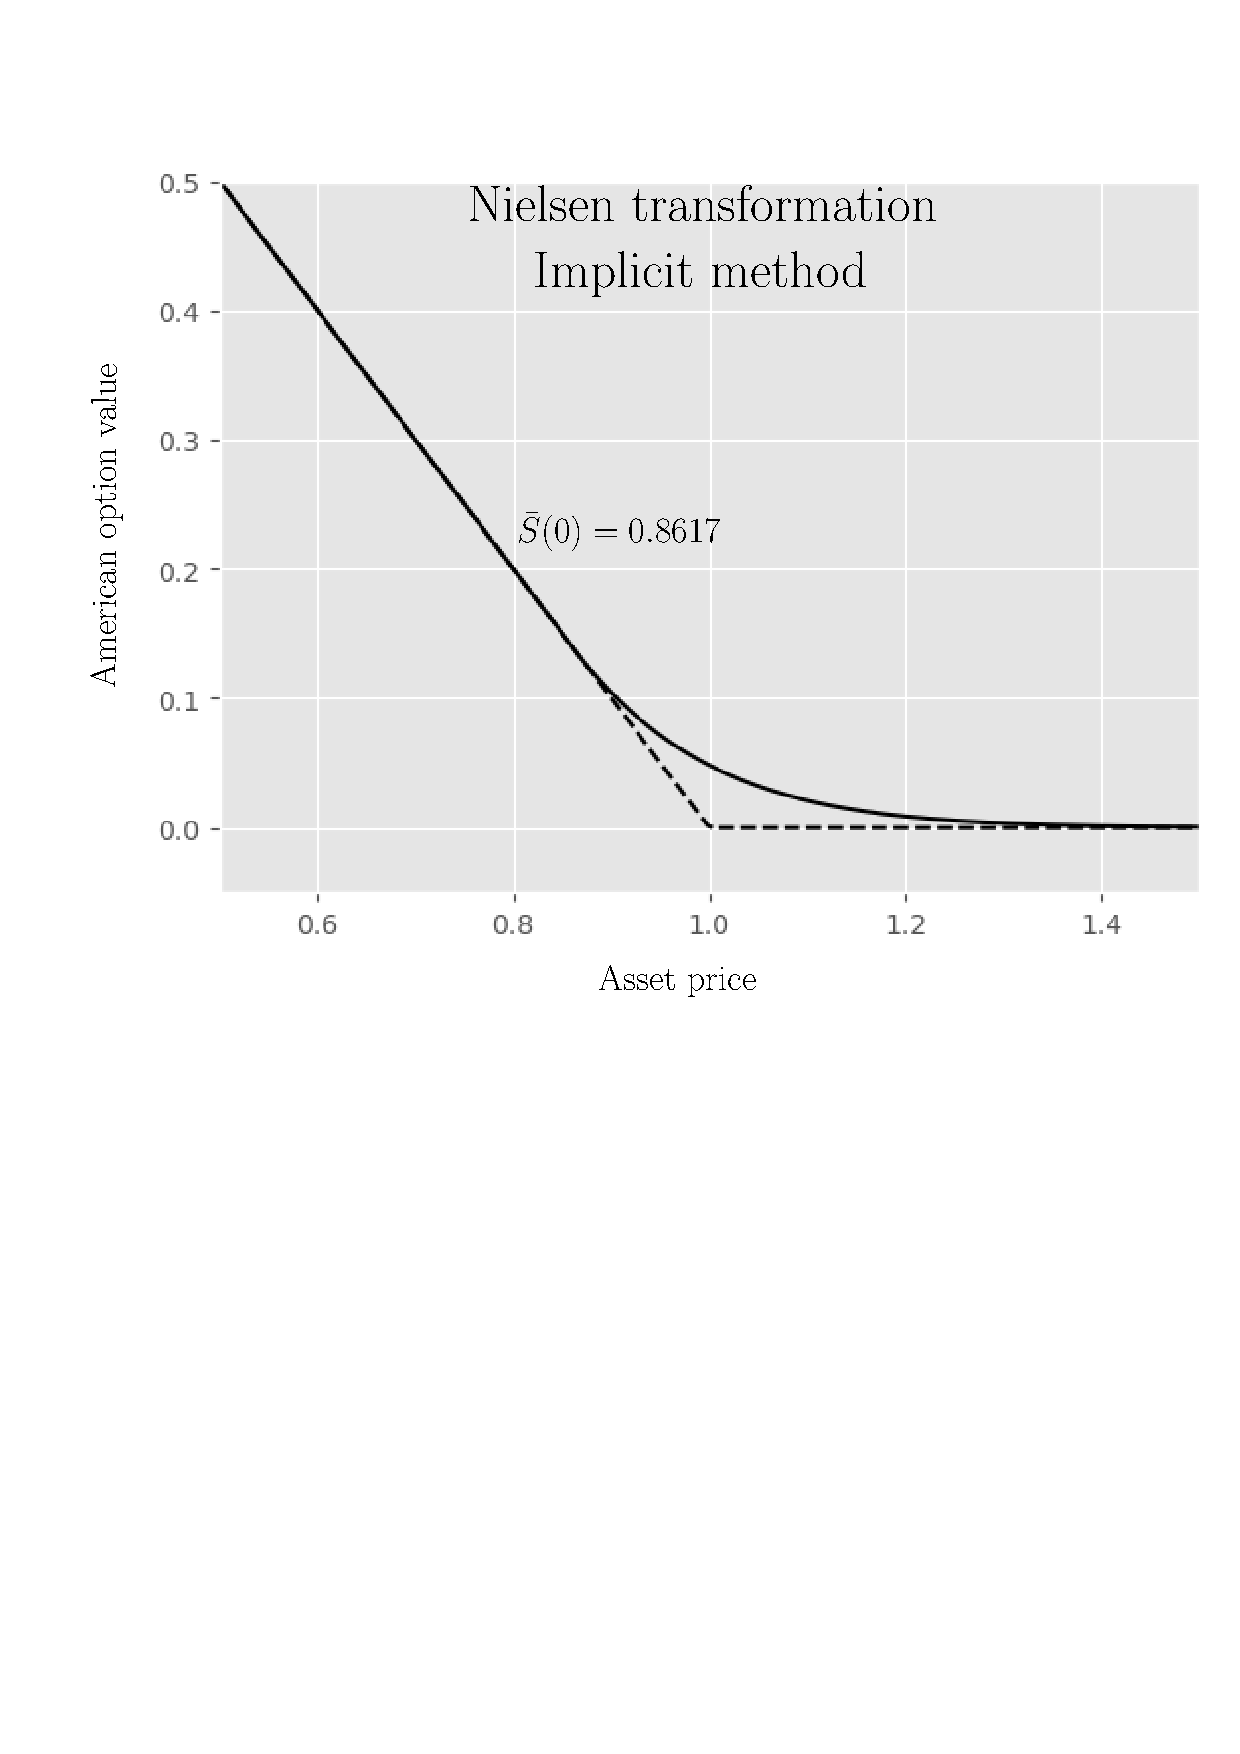
\includegraphics[width=\textwidth]{chapters/chapter3/TestCase2NielsenImplicit.pdf}
    \caption{$\Delta{x}=\Delta{t}=\expnumber{1}{-3}$.}
  \end{subfigure}
  \caption{American put option value $V(S, 0)$ given parameters \eqref{eq:numericaresults:parameters_set_1}.}
  \label{fig:finitedifferencesschemes:numericaresults:test_case_2}
\end{figure}

% Please add the following required packages to your document preamble:
% \usepackage{booktabs}
\begin{table}[H]
  \centering
  \begin{tabular}{@{}ccccc@{}}
  \toprule
  \textbf{Asset Price} &
    \textbf{BOPM} &
    \textbf{\begin{tabular}[c]{@{}c@{}}Explicit\\ Nielsen\end{tabular}} &
    \textbf{\begin{tabular}[c]{@{}c@{}}Implicit\\ Nielsen\end{tabular}} &
    \textbf{\begin{tabular}[c]{@{}c@{}}Explicit\\ Company\end{tabular}} \\ \midrule
  0.8 & 0.200000      & 0.200000 & 0.200000 & 0.200000 \\
  1.0 & 0.048167      & 0.048163 & 0.048944 & 0.048174 \\
  1.2 & 0.008666      & 0.008657 & 0.009290 & 0.008667 \\
  1.4 & 0.000167      & 0.001284 & 0.001519 & 0.001287 \\
  1.6 & 0.001285      & 0.000167 & 0.000229 & 0.000168 \\
  1.8 & 0.000020      & 0.000020 & 0.000033 & 0.000020 \\
  2.0 & 0.000002      & 0.000002 & 0.000005 & 0.000002 \\
      & \textbf{RSME} & 0.000005 & 0.000388 & 0.000003 \\
      & \textbf{Time} & 614ms    & 9891ms  & 68ms     \\ \bottomrule
  \end{tabular}
  \caption{\label{tab:rsme_explicit_company_transformation_2}  $V(S, 0)$ put approximation given parameters \eqref{eq:numericaresults:parameters_set_1}.}
\end{table}
The third numerical experiment was to price a call option with dividends
\begin{equation}
  \label{eq:numericaresults:parameters_set_3}
  K = 1, \quad T = 1, \quad r=0.2, \quad \sigma=0.2, \quad \delta = 0.09
\end{equation}
\begin{figure}[H]
  \centering
  \begin{subfigure}{0.4\textwidth}
    \centering
    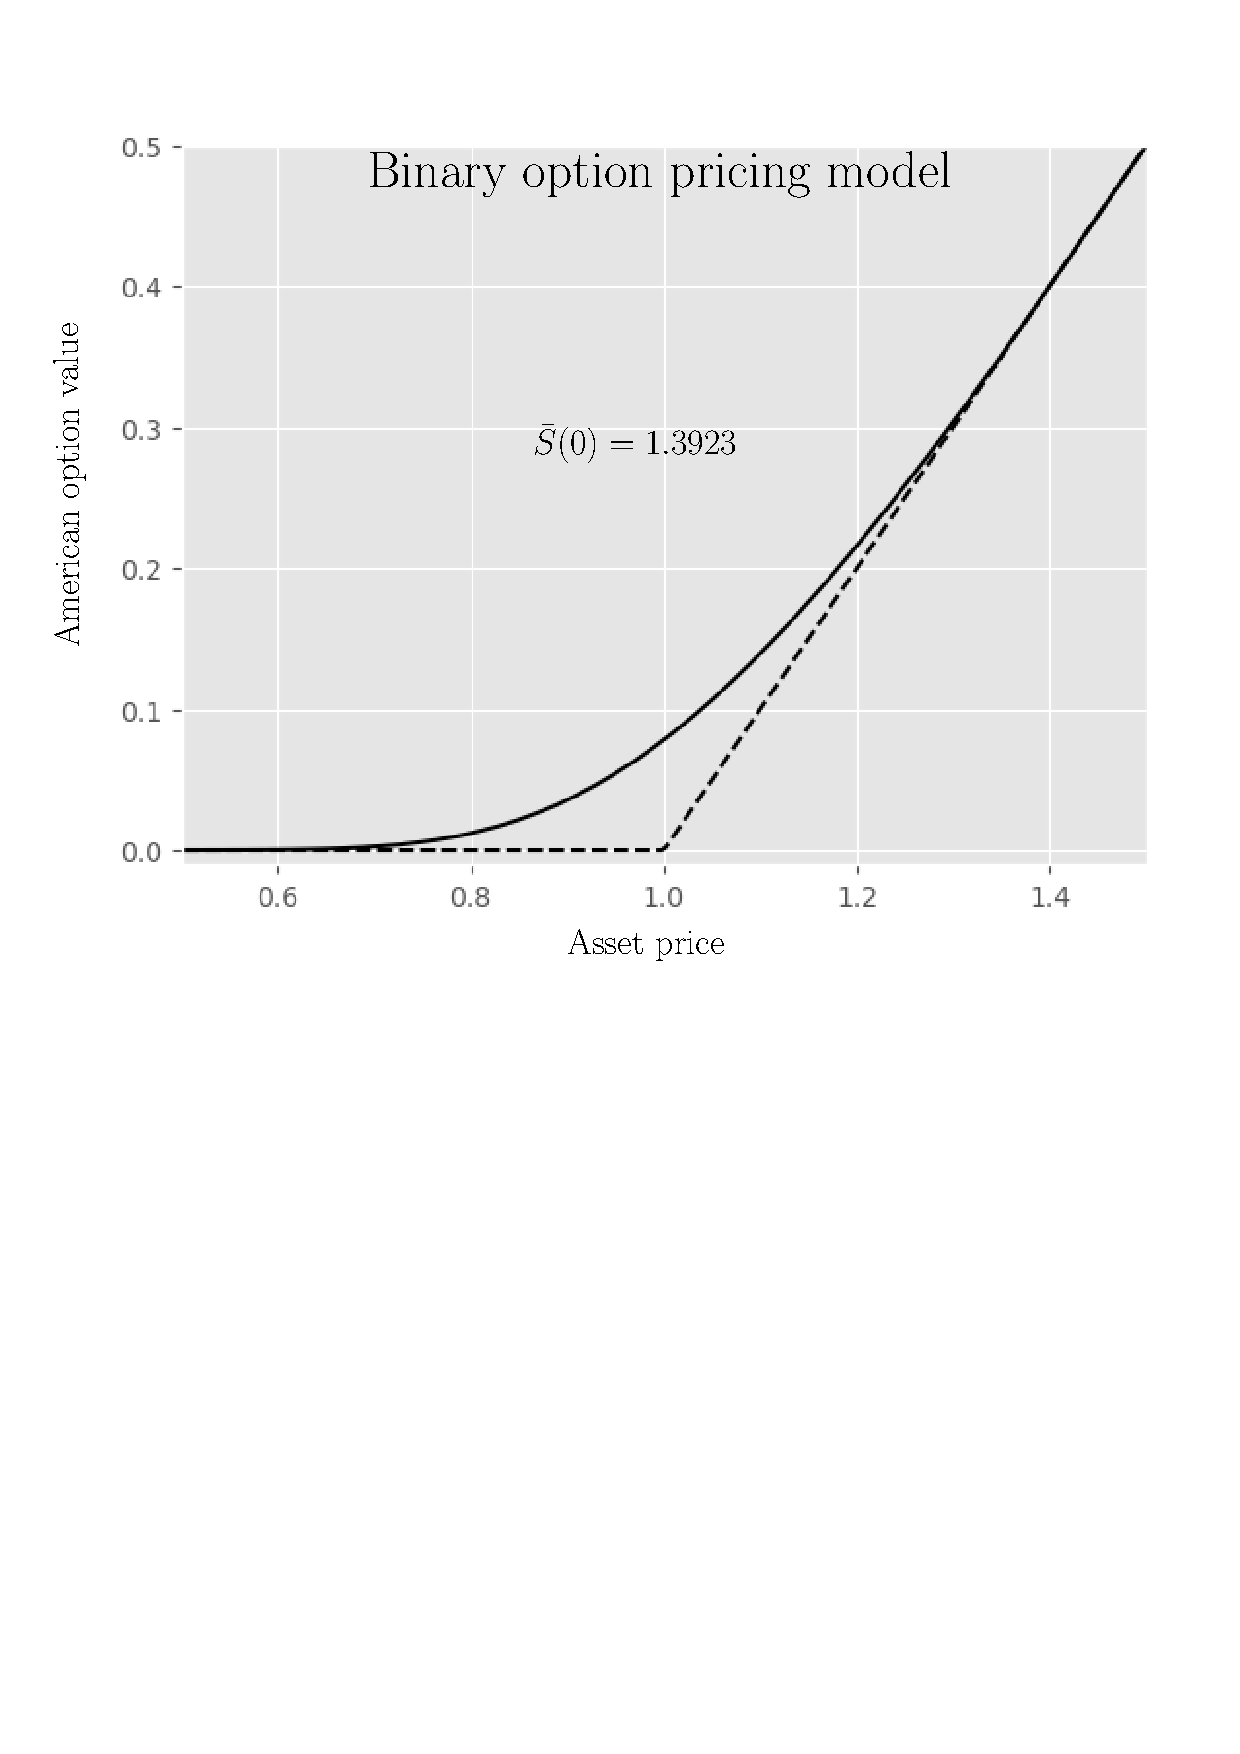
\includegraphics[width=\textwidth]{chapters/chapter3/TestCase3BOPM.pdf}
    \caption{$\text{Nodes} = 2^{500}$.}
    \label{fig:finitedifferencesschemes:numericaresults:test_case_3_bopm}
  \end{subfigure}
  \hspace{0.5cm}
  \begin{subfigure}{0.4\textwidth}
    \centering
    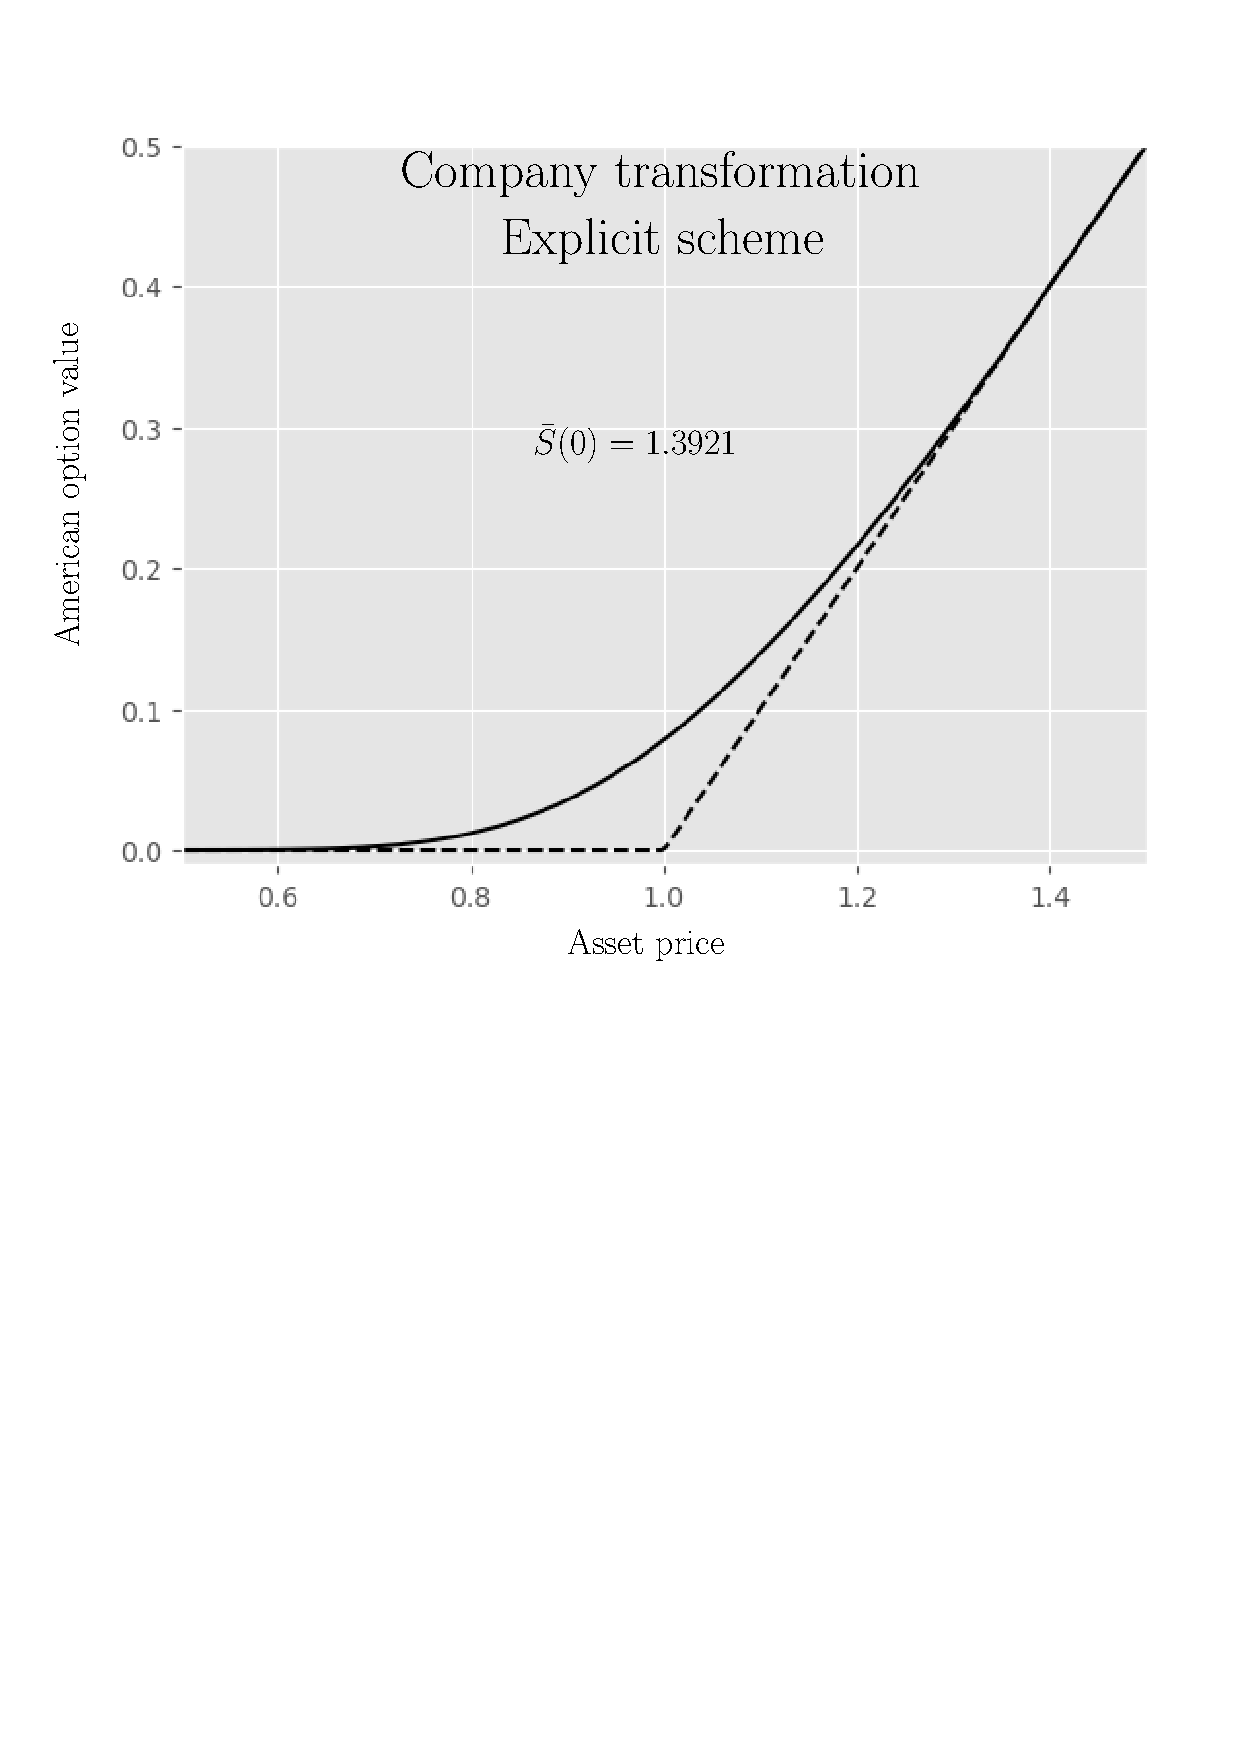
\includegraphics[width=\textwidth]{chapters/chapter3/TestCase3ExplicitCompany.pdf}
    \caption{$\Delta{x}=\expnumber{1}{-3}, \Delta{t}=0.5\times\expnumber{1}{-6}$}
    \label{fig:finitedifferencesschemes:numericaresults:test_case_3_explicit_company}
  \end{subfigure}
  \begin{subfigure}{0.4\textwidth}
    \centering
    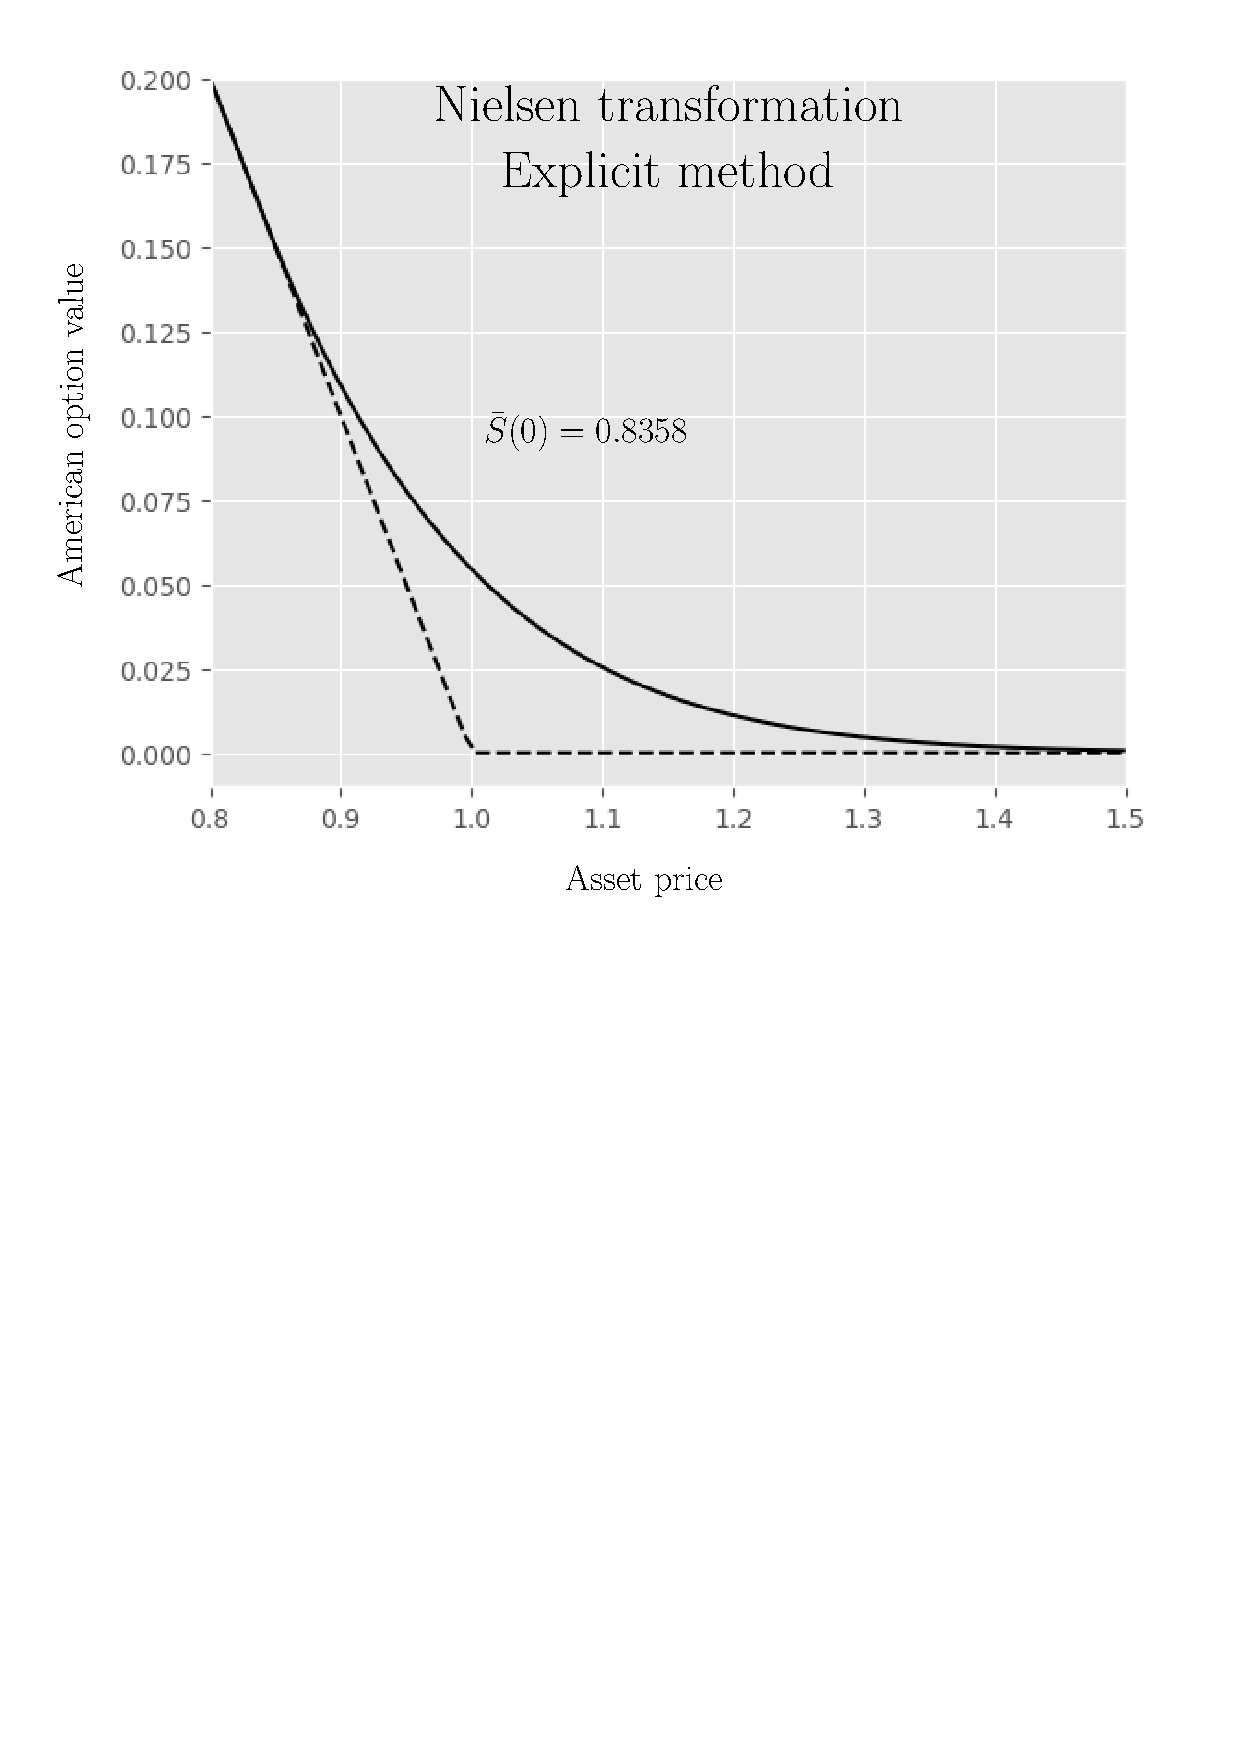
\includegraphics[width=\textwidth]{chapters/chapter3/TestCase3ExplicitNielsen.pdf}
    \caption{$\Delta{x}=\expnumber{1}{-3}, \Delta{t}=0.5\times\expnumber{1}{-6}$}
    \label{fig:finitedifferencesschemes:numericaresults:test_case_3_explicit_nielsen}
  \end{subfigure}
  \hspace{0.5cm}
  \begin{subfigure}{0.4\textwidth}
    \label{fig:finitedifferencesschemes:numericaresults:test_case_3_implicit_nielsen}
    \centering
    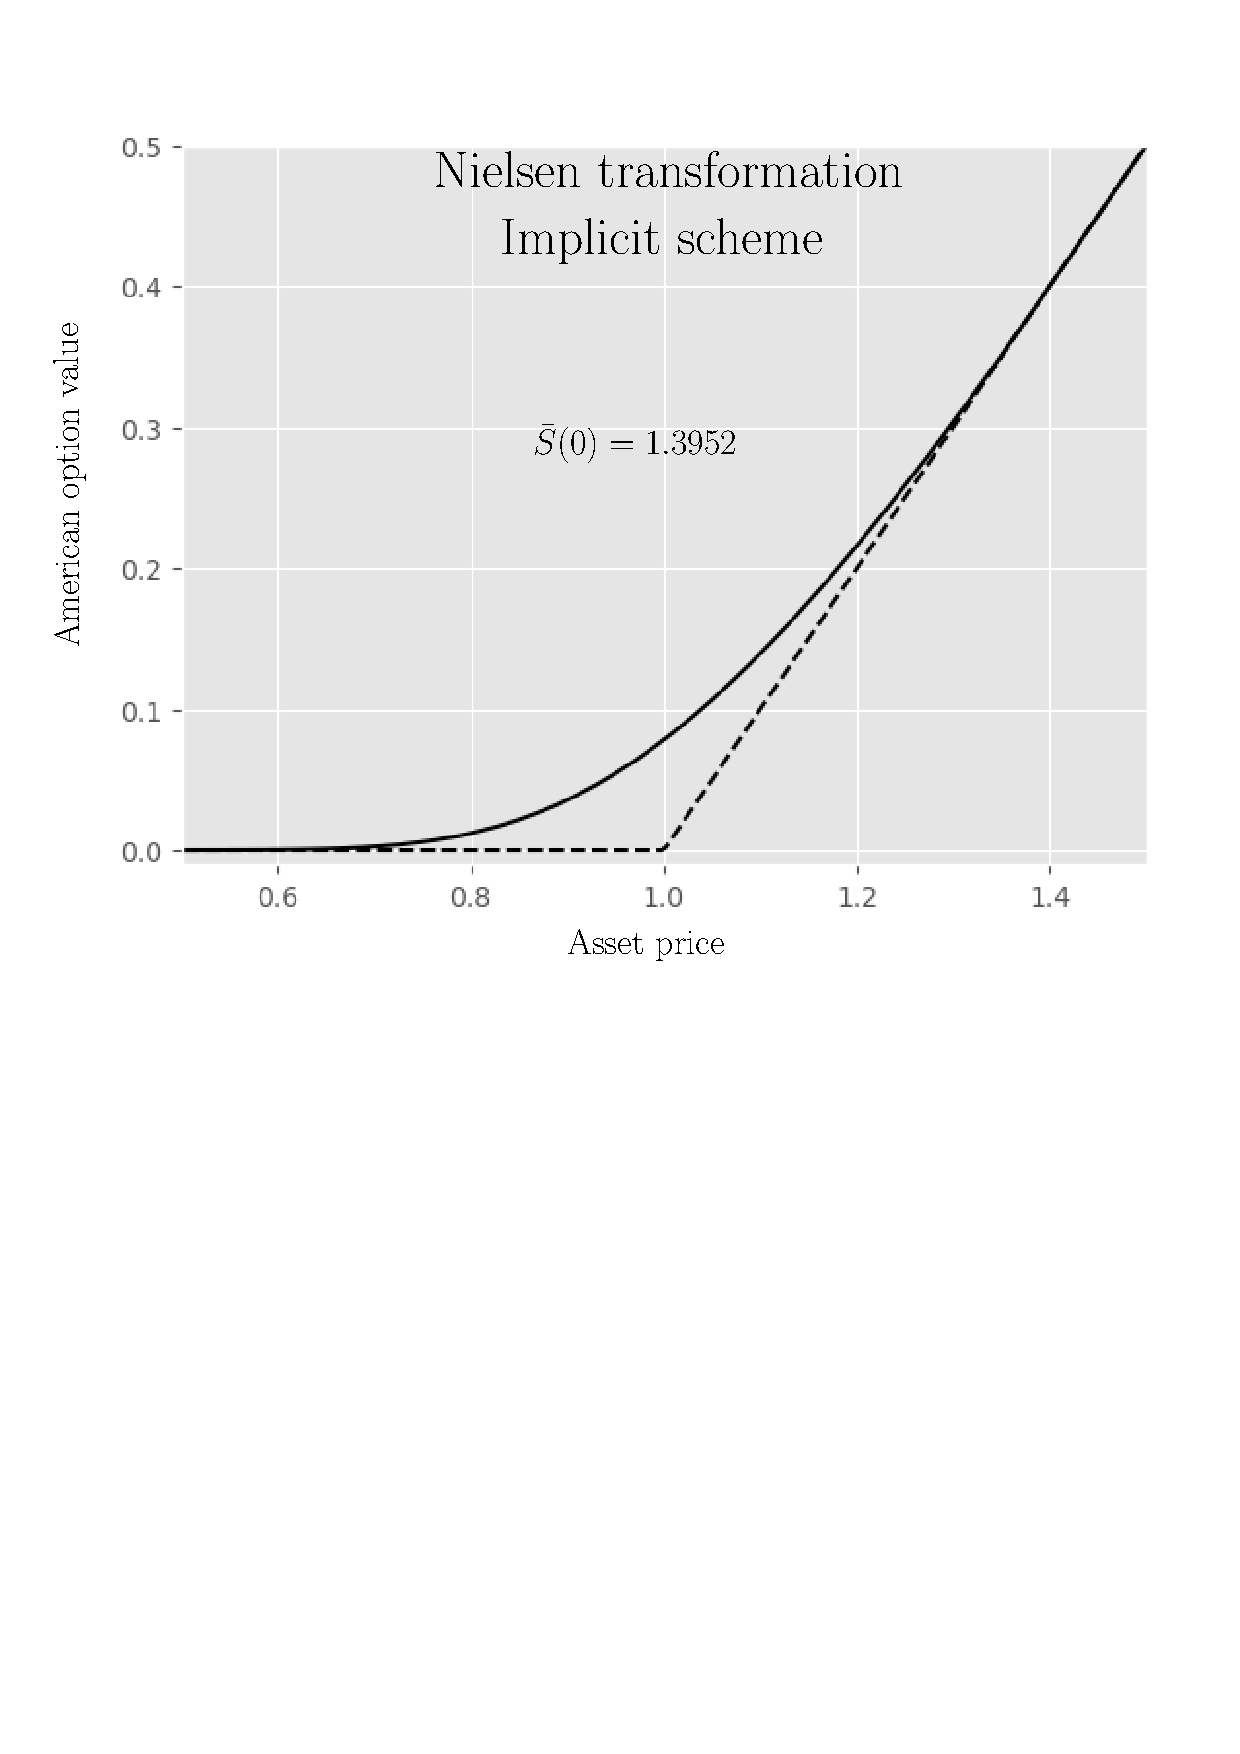
\includegraphics[width=\textwidth]{chapters/chapter3/TestCase3ImplicitNielsen.pdf}
    \caption{$\Delta{x}=\Delta{t}=\expnumber{1}{-3}$.}
  \end{subfigure}
  \caption{American call option value $V(S, 0)$ given parameters \eqref{eq:numericaresults:parameters_set_3}.}
  \label{fig:finitedifferencesschemes:numericaresults:test_case_3}
\end{figure}
% Please add the following required packages to your document preamble:
% \usepackage{booktabs}
\begin{table}[H]
  \centering
  \begin{tabular}{@{}ccccc@{}}
  \toprule
  \textbf{Asset Price} &
    \textbf{BOPM} &
    \textbf{\begin{tabular}[c]{@{}c@{}}Explicit\\ Nielsen\end{tabular}} &
    \textbf{\begin{tabular}[c]{@{}c@{}}Implicit\\ Nielsen\end{tabular}} &
    \textbf{\begin{tabular}[c]{@{}c@{}}Explicit\\ Company\end{tabular}} \\ \midrule
  0.4 & 0.0000000 & 0.0000002 & 0.000083 & 0.0000000 \\
  0.6 & 0.0002771 & 0.0002712 & 0.002238 & 0.0002763 \\
  0.8 & 0.0119621 & 0.0119311 & 0.011796 & 0.0119633 \\
  1.0 & 0.0780630 & 0.0780630 & 0.078109 & 0.0780628 \\
  1.2 & 0.2159015 & 0.2159348 & 0.215718 & 0.2159007 \\
  1.4 & 0.4000000 & 0.3999589 & 0.400443 & 0.4000000 \\
      & \textbf{RSME} & 0.000006 & 0.00203 & 0.000000 \\
      & \textbf{Time} & 512ms    & 10132ms  & 83ms     \\ \bottomrule
  \end{tabular}
  \caption{\label{tab:rsme_explicit_company_transformation_3} $V(S, 0)$ call approximation given parameters \eqref{eq:numericaresults:parameters_set_3}.}
\end{table}

Finally, we also price a put option with dividends using parameters
\begin{equation}
  \label{eq:numericaresults:parameters_set_4}
  K = 1, \quad T = 1, \quad r=0.2, \quad \sigma=0.2, \quad \delta = 0.03
\end{equation}
\begin{figure}[H]
  \centering
  \begin{subfigure}{0.4\textwidth}
    \centering
    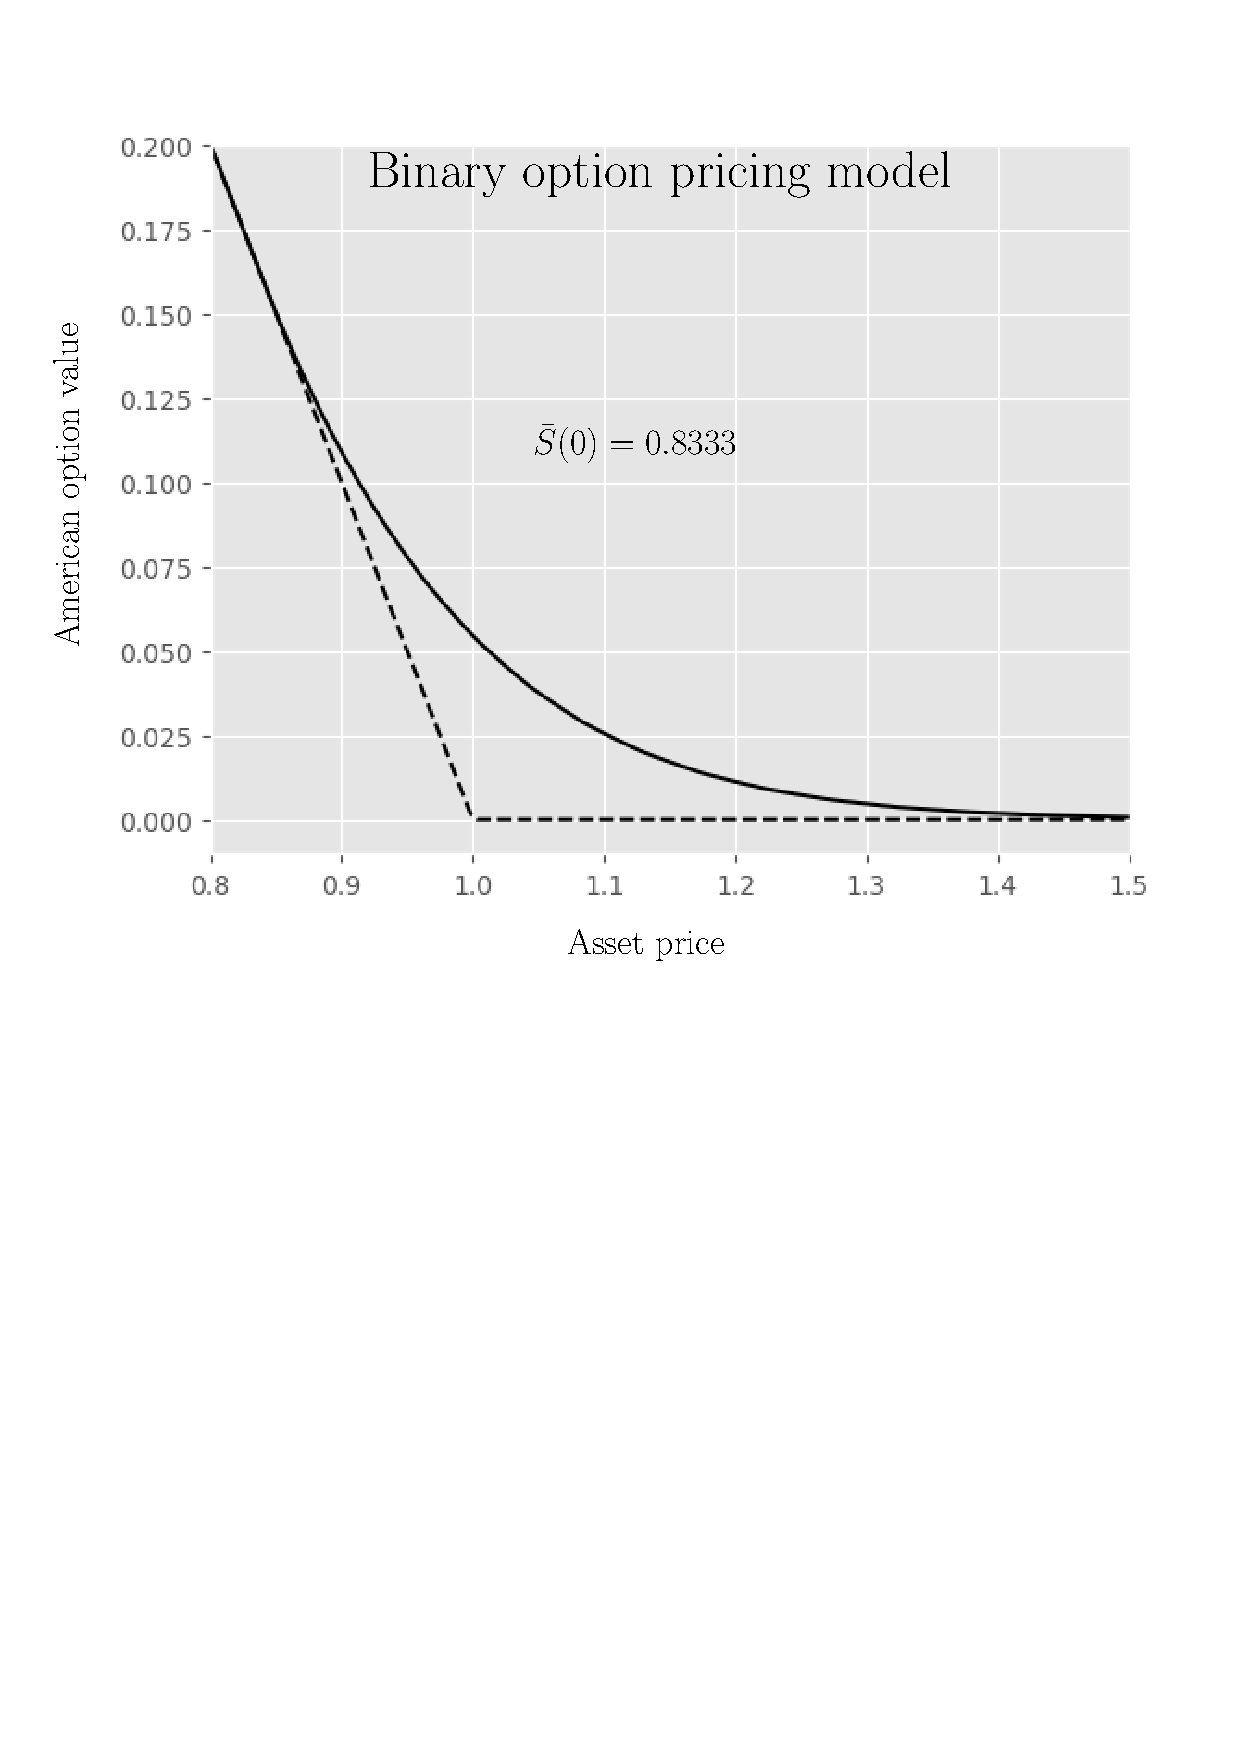
\includegraphics[width=\textwidth]{chapters/chapter3/TestCase4BOPM.pdf}
    \caption{$\text{Nodes} = 2^{500}$.}
    \label{fig:finitedifferencesschemes:numericaresults:test_case_4_bopm}
  \end{subfigure}
  \hspace{0.5cm}
  \begin{subfigure}{0.4\textwidth}
    \centering
    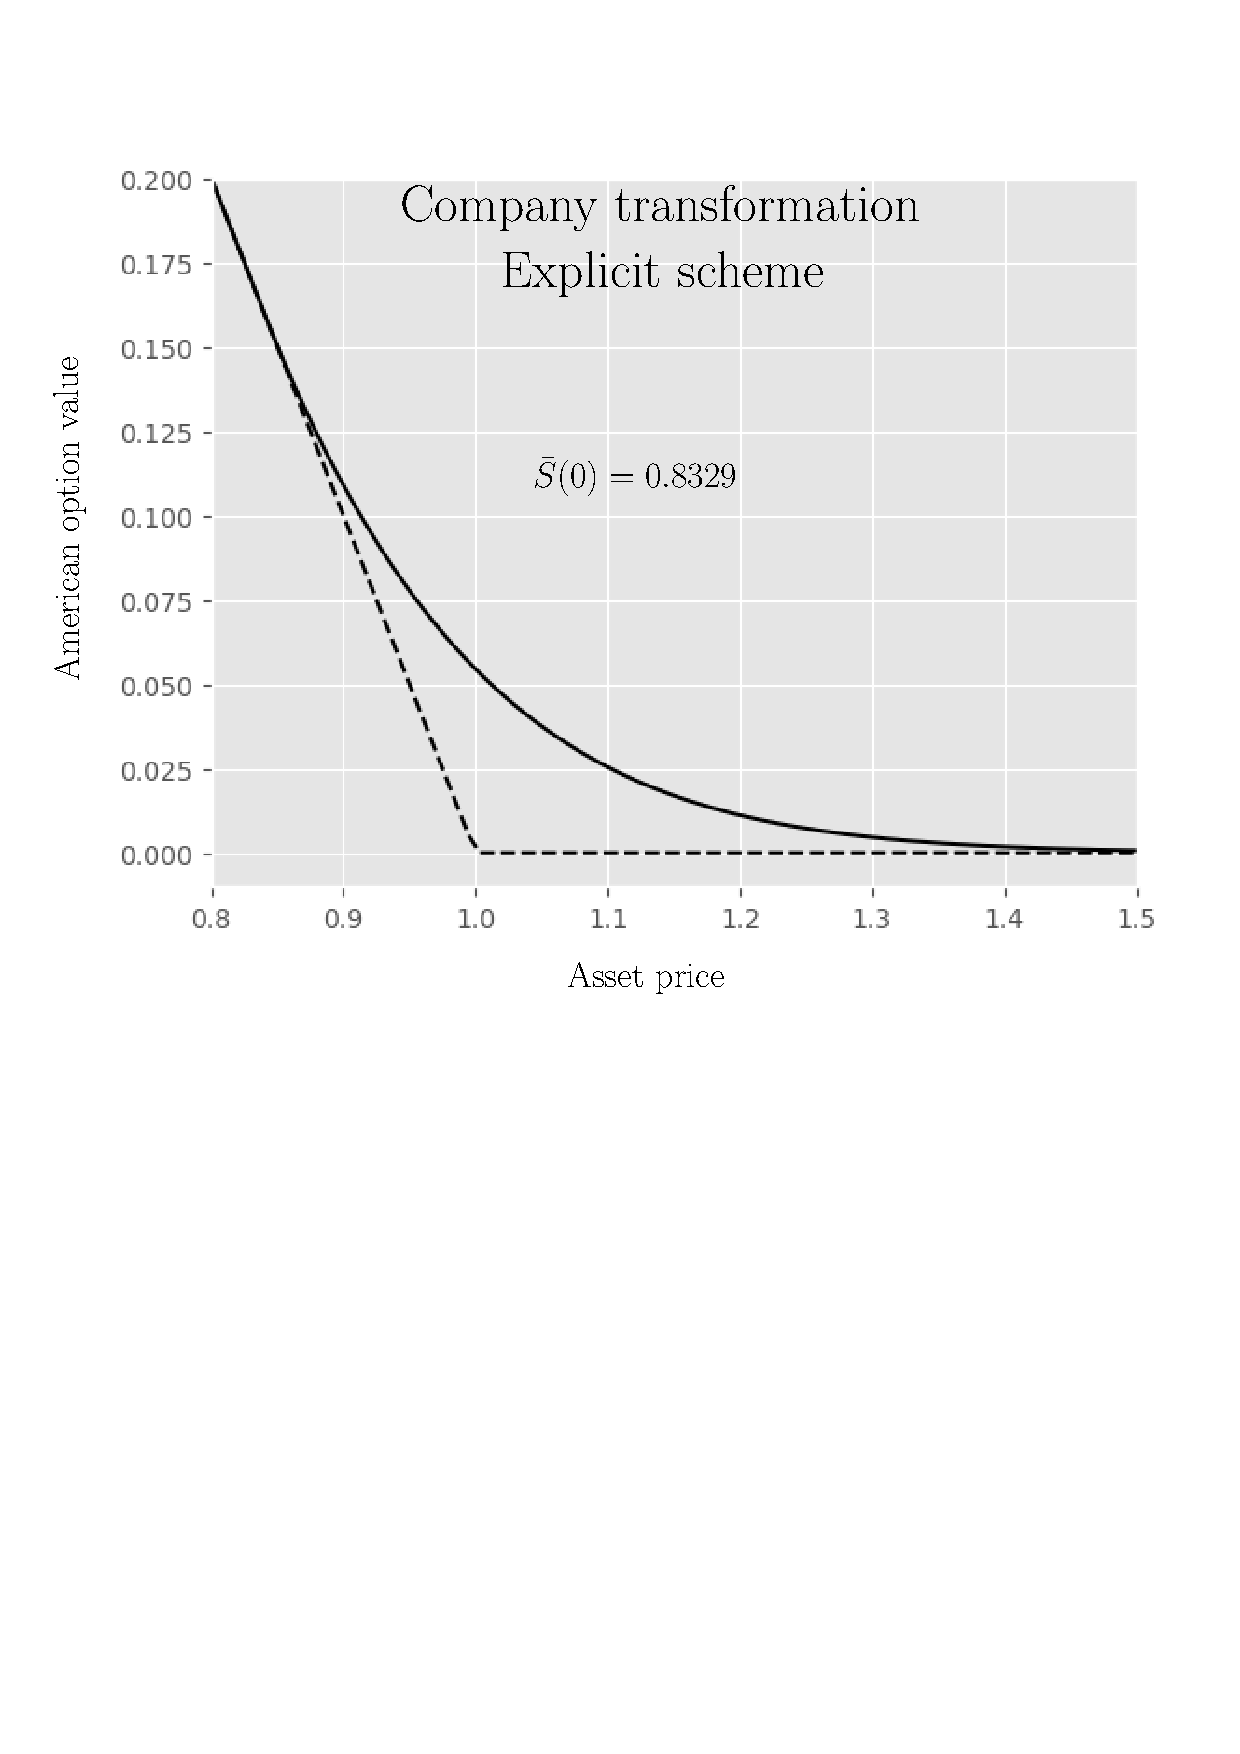
\includegraphics[width=\textwidth]{chapters/chapter3/TestCase4ExplicitCompany.pdf}
    \caption{$\Delta{x}=\expnumber{1}{-3}, \Delta{t}=0.5\times\expnumber{1}{-6}$}
    \label{fig:finitedifferencesschemes:numericaresults:test_case_4_explicit_company}
  \end{subfigure}
  \begin{subfigure}{0.4\textwidth}
    \centering
    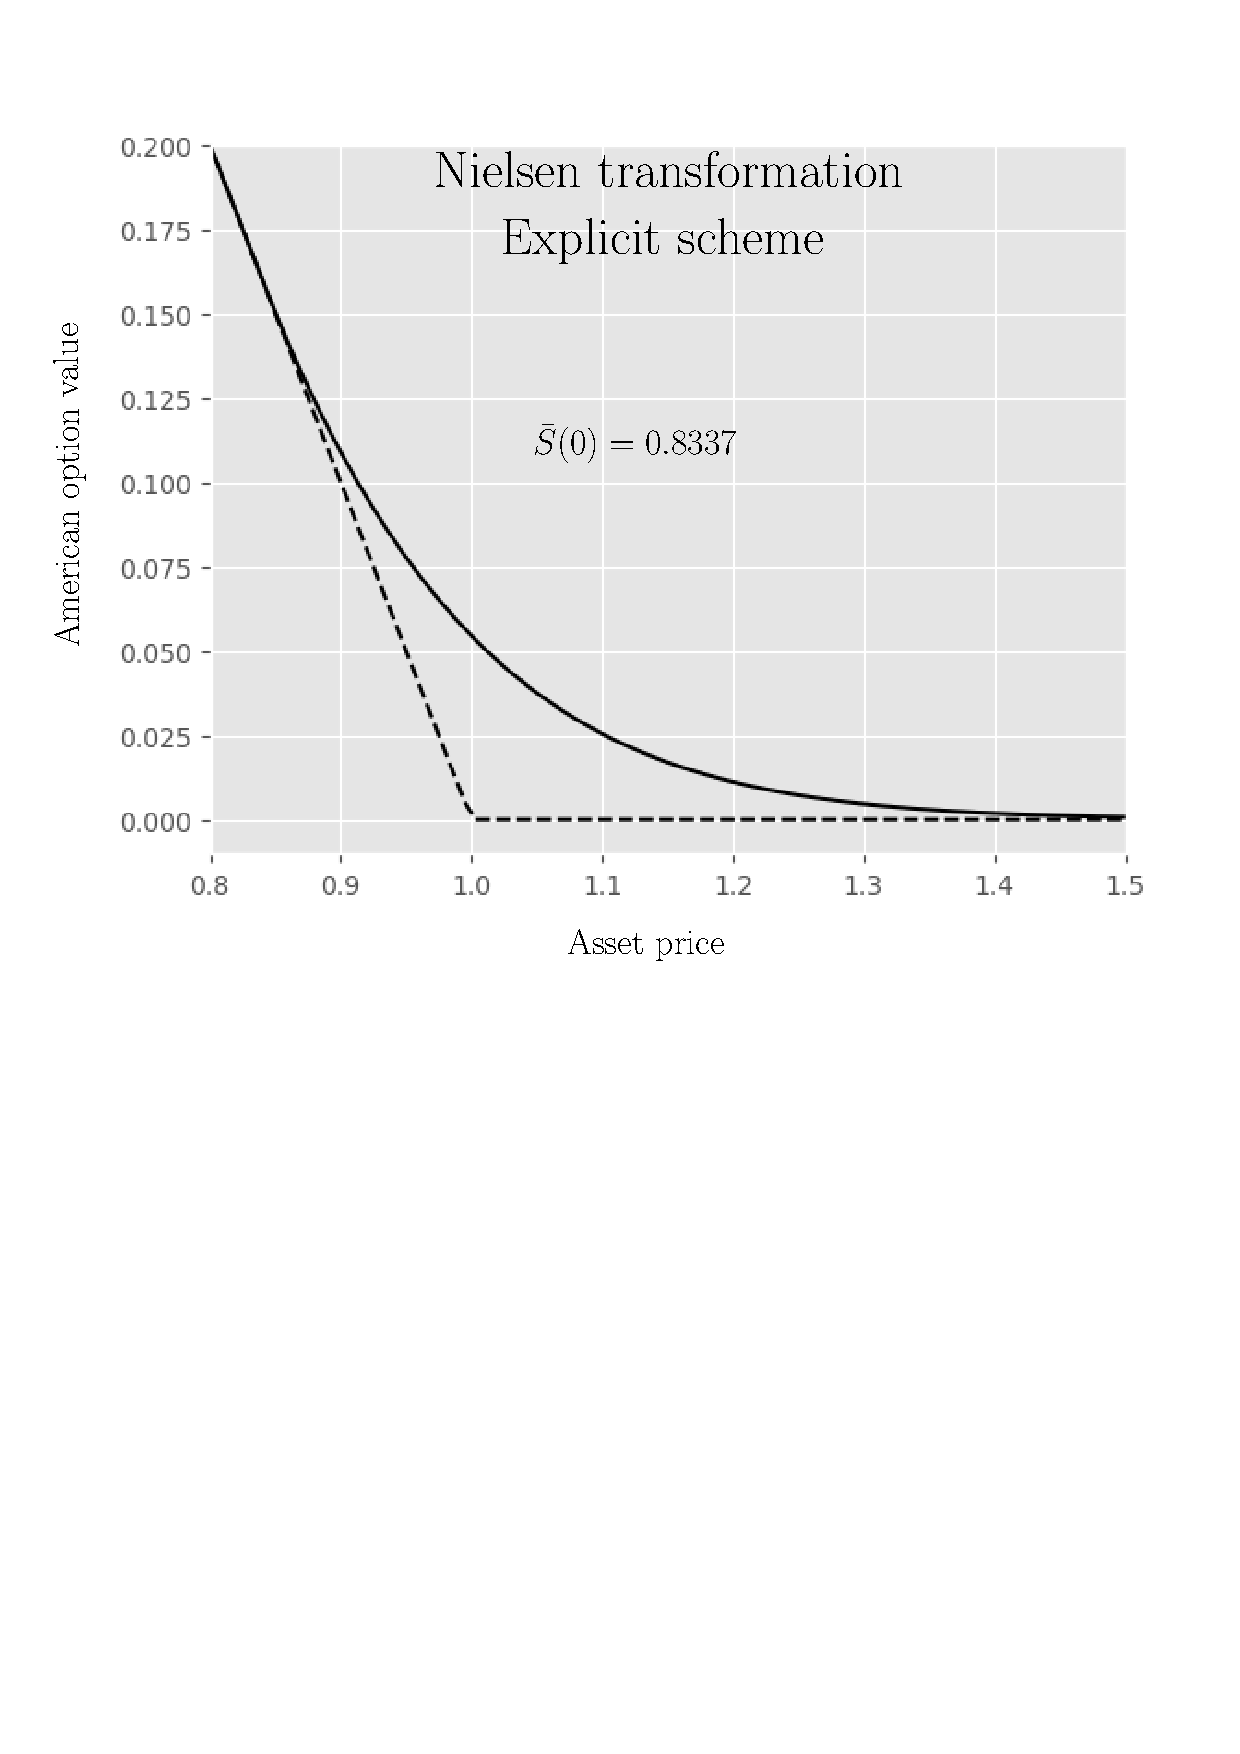
\includegraphics[width=\textwidth]{chapters/chapter3/TestCase4ExplicitNielsen.pdf}
    \caption{$\Delta{x}=\expnumber{1}{-3}, \Delta{t}=0.5\times\expnumber{1}{-6}$}
    \label{fig:finitedifferencesschemes:numericaresults:test_case_4_explicit_nielsen}
  \end{subfigure}
  \hspace{0.5cm}
  \begin{subfigure}{0.4\textwidth}
    \label{fig:finitedifferencesschemes:numericaresults:test_case_4_implicit_nielsen}
    \centering
    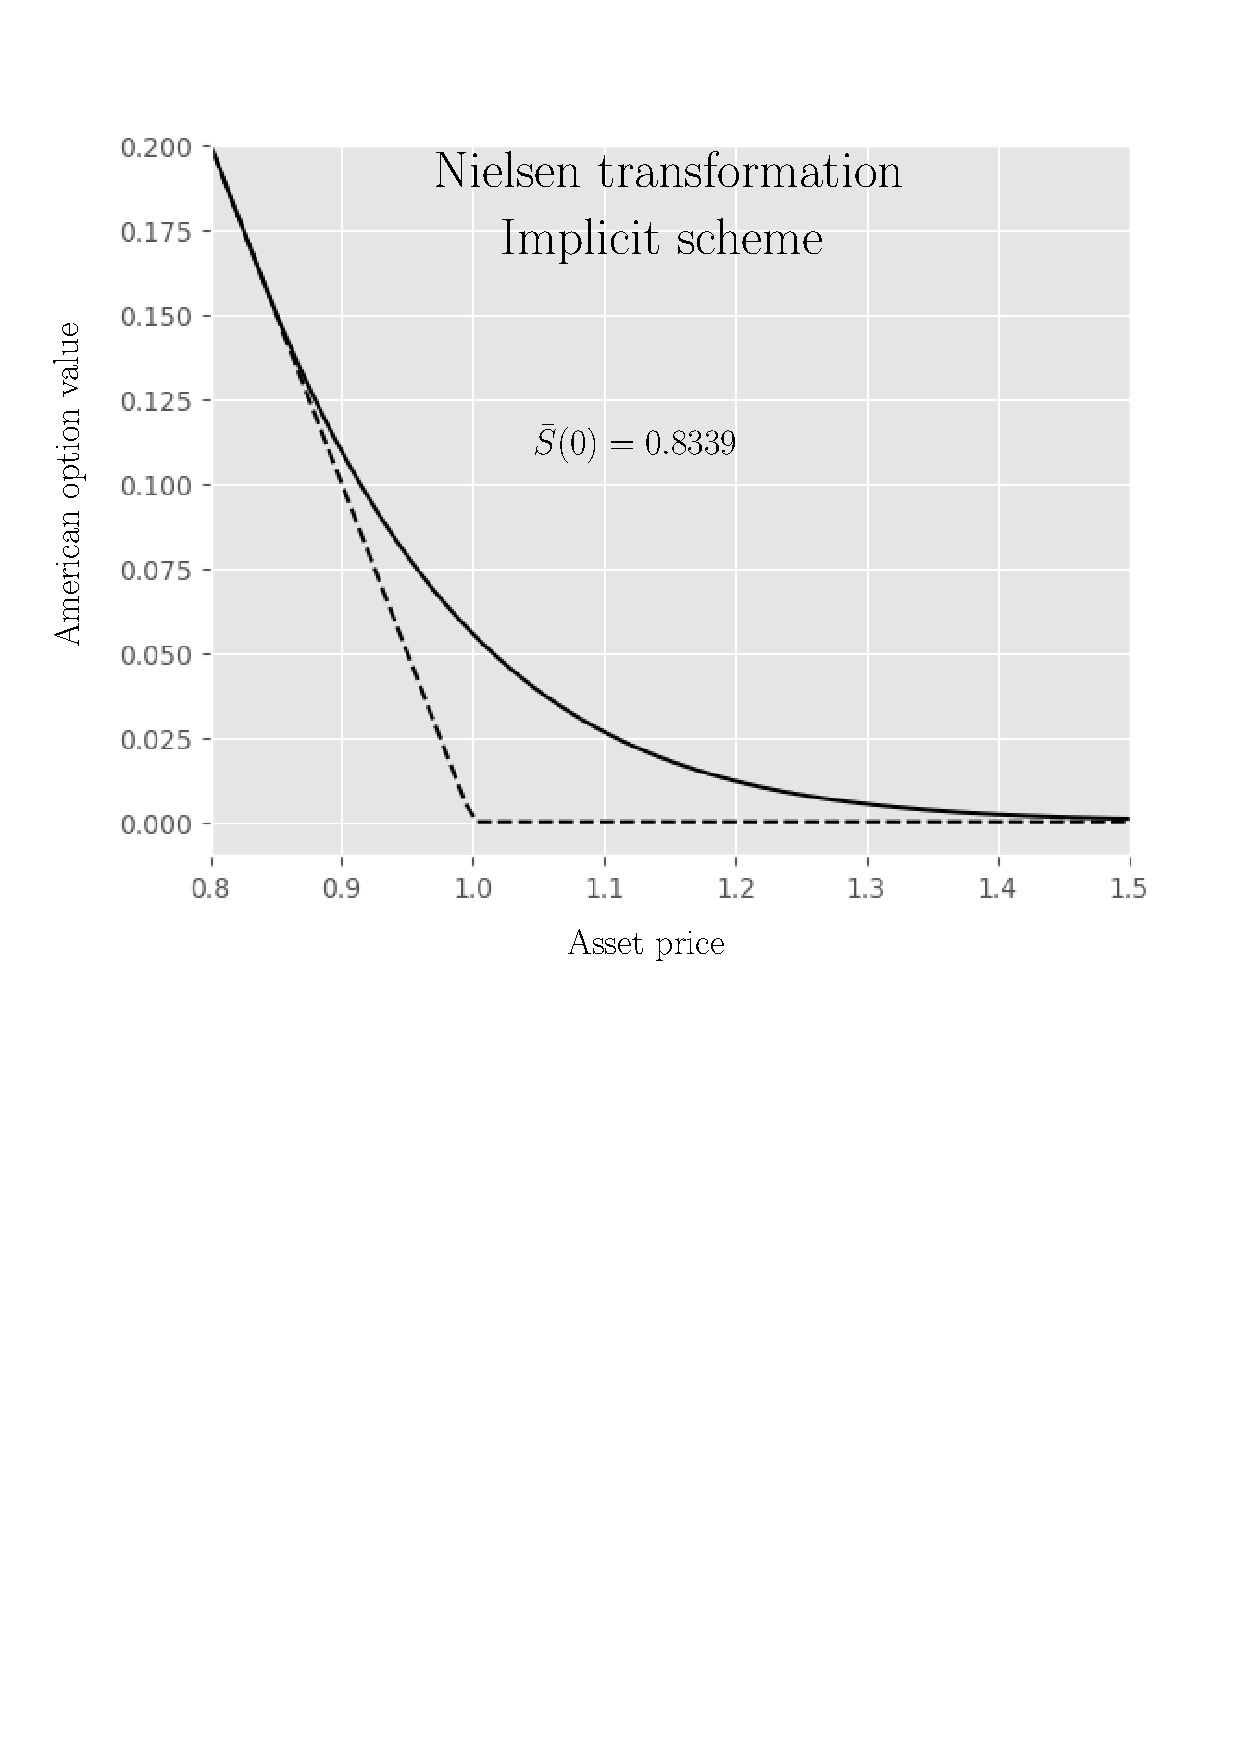
\includegraphics[width=\textwidth]{chapters/chapter3/TestCase4ImplicitNielsen.pdf}
    \caption{$\Delta{x}=\Delta{t}=\expnumber{1}{-3}$.}
  \end{subfigure}
  \caption{American put option value $V(S, 0)$ curve.}
  \label{fig:finitedifferencesschemes:numericaresults:test_case_4}
\end{figure}

% Please add the following required packages to your document preamble:
% \usepackage{booktabs}
\begin{table}[H]
  \centering
  \begin{tabular}{@{}ccccc@{}}
    \toprule
    \textbf{Asset Price} &
      \textbf{BOPM} &
      \textbf{\begin{tabular}[c]{@{}c@{}}Explicit\\ Nielsen\end{tabular}} &
      \textbf{\begin{tabular}[c]{@{}c@{}}Implicit\\ Nielsen\end{tabular}} &
      \textbf{\begin{tabular}[c]{@{}c@{}}Explicit\\ Company\end{tabular}} \\ \midrule
    0.6 & 0.400000      & 0.400000 & 0.400000 & 0.400000 \\
    0.8 & 0.200000      & 0.200000 & 0.200000 & 0.200000 \\
    1.0 & 0.054464      & 0.054469 & 0.055593 & 0.054491 \\
    1.2 & 0.011255      & 0.011161 & 0.012096 & 0.011167 \\
    1.4 & 0.001855      & 0.001847 & 0.002225 & 0.001850 \\
    1.6 & 0.000262      & 0.000265 & 0.000373 & 0.000266 \\
        & \textbf{RMSE} & 0.000031 & 0.000486 & 0.000031 \\
        & \textbf{Time} & 416ms    & 29581ms  & 194ms    \\ \bottomrule
    \end{tabular}
  \caption{\label{tab:rsme_explicit_company_transformation_4} $V(S, 0)$ put approximation given parameters \eqref{eq:numericaresults:parameters_set_4}.}
\end{table}

Summarizing, none of the front fixing schemes can be used to price American call options without dividends. The explicit schemes are much faster than the implicit scheme. Nielsen explicit scheme is less accurate than Company explicit scheme. We will see later that Company explicit scheme is second order in space. Therefore, it converges faster than Nielsen explicit scheme. Moreover, the Nielsen is slower because at each time step it has to compute the term $D^{n+1}_i$ for $i=0,\dots,M+1$ (See line 9-10 in algorithms \eqref{alg:finitedifferencesschemes:explicit:call_explicit_method_algorithm} and \eqref{alg:finitedifferencesschemes:explicit:put_explicit_method_algorithm}) while the Company does not (See algorithms \eqref{alg:appendix:companytransformation:explicits:call_explicit_method_algorithm}
and \eqref{alg:appendix:companytransformation:explicits:put_explicit_method_algorithm}).

\subsubsection{Convergence analysis}

We conducted a convergence analysis to determine the order of convergence of each the methods. For simplicity, the numerical experiment was conducted for put options and with parameters \eqref{eq:numericaresults:parameters_set_4}. We expect that numerical experiments yield similar results for call options and other set of parameters. Moreover, for analyzing the convergence, we are taking the relative error between contiguous grid in sizes. Specifically, to determine the order of convergence in space, we define the grids with resolution $\Delta{x}_i=h/2^i$ for $i=0,\dots,3$ while $\Delta{t}$ is fixed. Conversely, to determine the temporal order of convergence, we vary $\Delta{t}$ and fix $\Delta{x}$ in similar way. Therefore, the error between consecutive grids is defined as
\begin{equation}
  \mathbf{e}_k = ||\mathbf{v}_{k+1} - \mathbf{v}_{k}||_{\infty} \quad \text{for $k=0,\dots,3$}
  \label{eq:finitedifferencesschemes:numericalresults:consecutive_error}
\end{equation}
where $\mathbf{v}_{k}\in\mathbb{R}^{M+1}$ is the vector with the approximation produced by our method and $||\cdot||_{\infty}$ is the infinity norm. In figure \eqref{fig:finitedifferencesschemes:numericaresults:nielsen_convergence analysis}, we show log-log plots of the error produced by the explicit and implicit methods for Nielsen transformation. As you can see, both explicit and implicit methods have first order convergence in space. Recall that although we are using central finite difference, the Nielsen schemes use forward (or backward for calls) difference to approximate the contact point condition \eqref{eq:finitedifferencesschemes:explicit:contact_point_approximation_2} which is first order in space, hence, degrading the overall convergence of the method. In the other hand, figure \eqref{fig:finitedifferencesschemes:numericaresults:company_convergence analysis} shows the convergence order for the explicit method for the Company transformation. Contrary to Nielsen's schemes, the explicit method for Company transformation is second order in space. This is because Company uses a central finite difference scheme for approximating the contact point condition \eqref{eq:appendix:explicitmethodcompany:contact_point_approximation}. Moreover, all the schemes are first order convergence in space as suggested by the forward/backward difference approximation used for the temporal axis.
\begin{figure}[tbp]
  \centering
  \begin{subfigure}{0.4\textwidth}
    \centering
    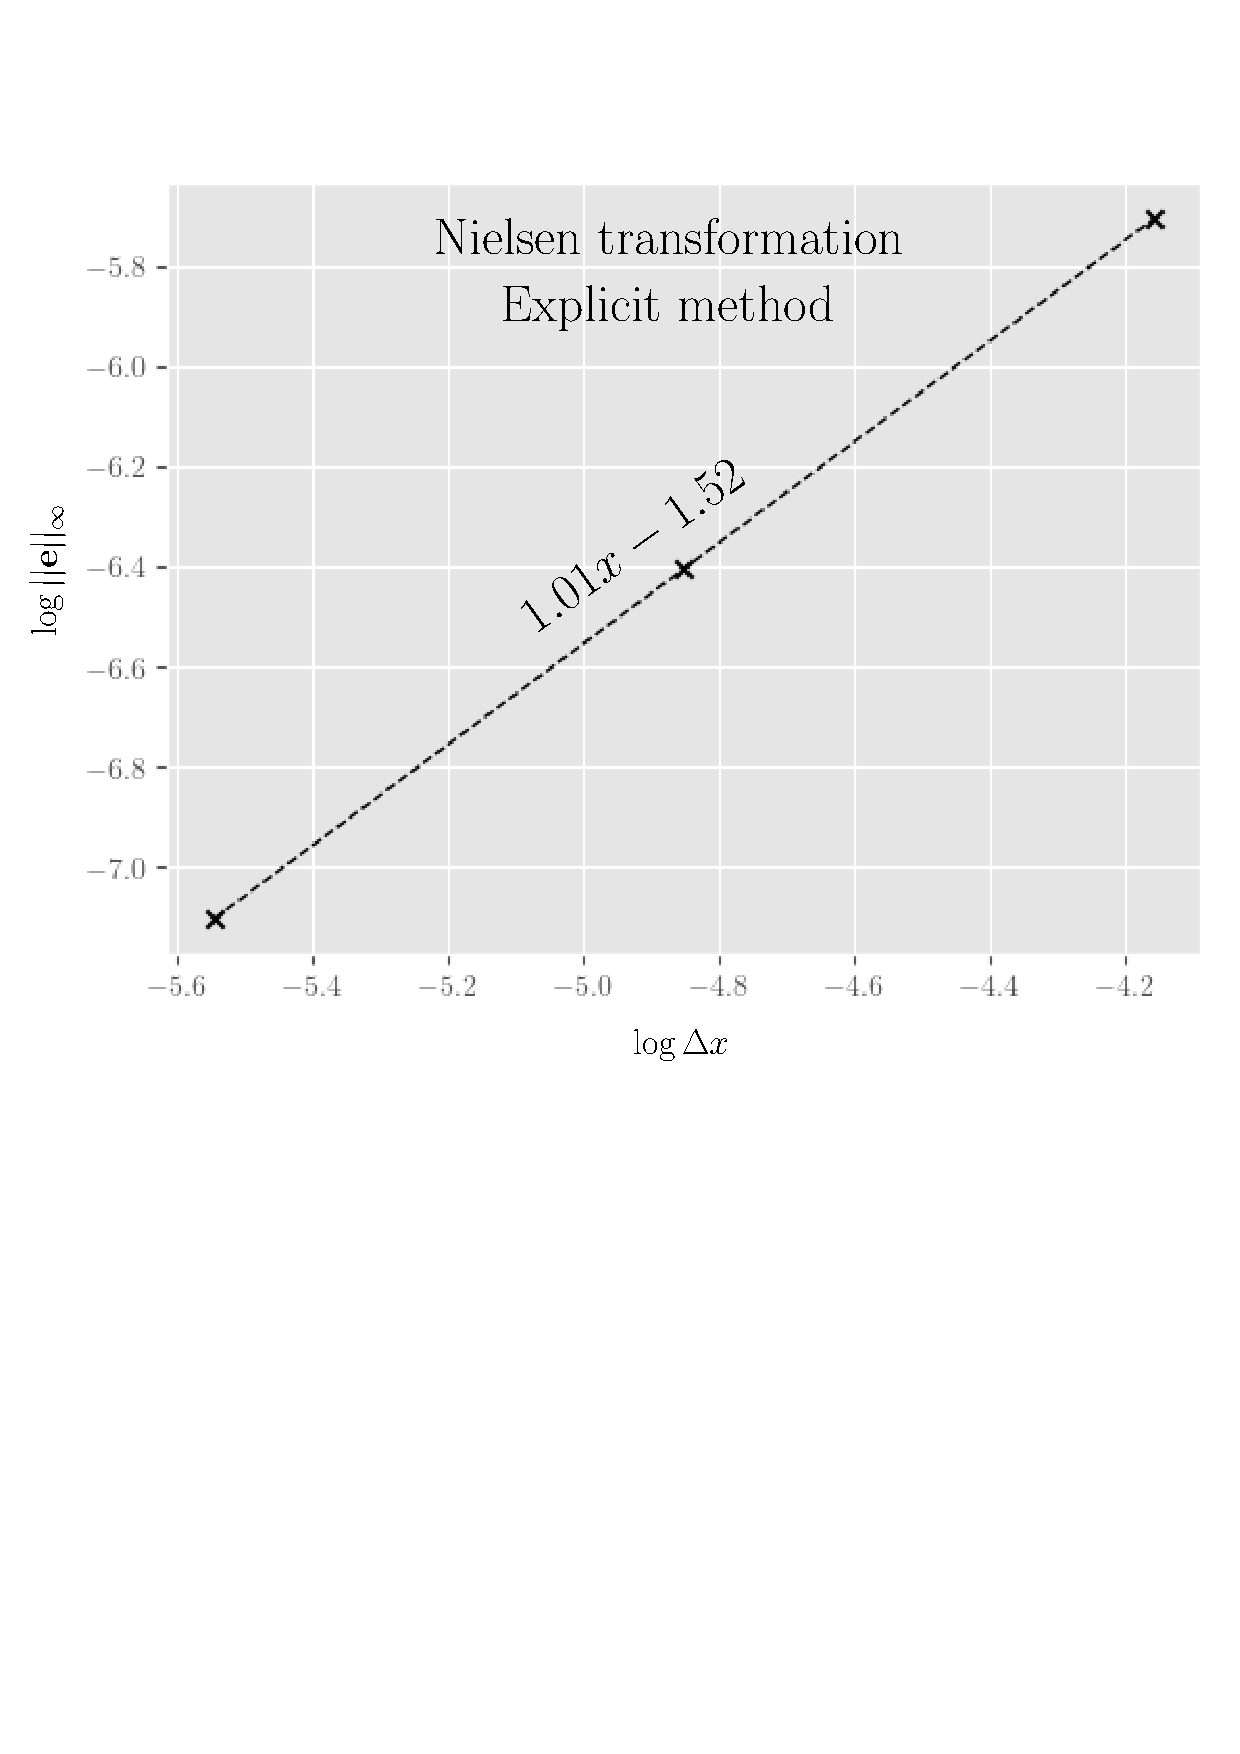
\includegraphics[width=\textwidth]{chapters/chapter3/ConvergenceSpaceExplicitNielsen.pdf}
    \caption{$\Delta{x}=2^{-7},\dots,2^{-10}$}
    \caption*{$\Delta{t}=2^{-21}$}
    \label{fig:finitedifferencesschemes:numericaresults:nielsen_explicit_space}
  \end{subfigure}
  \hspace{0.5cm}
  \begin{subfigure}{0.4\textwidth}
    \centering
    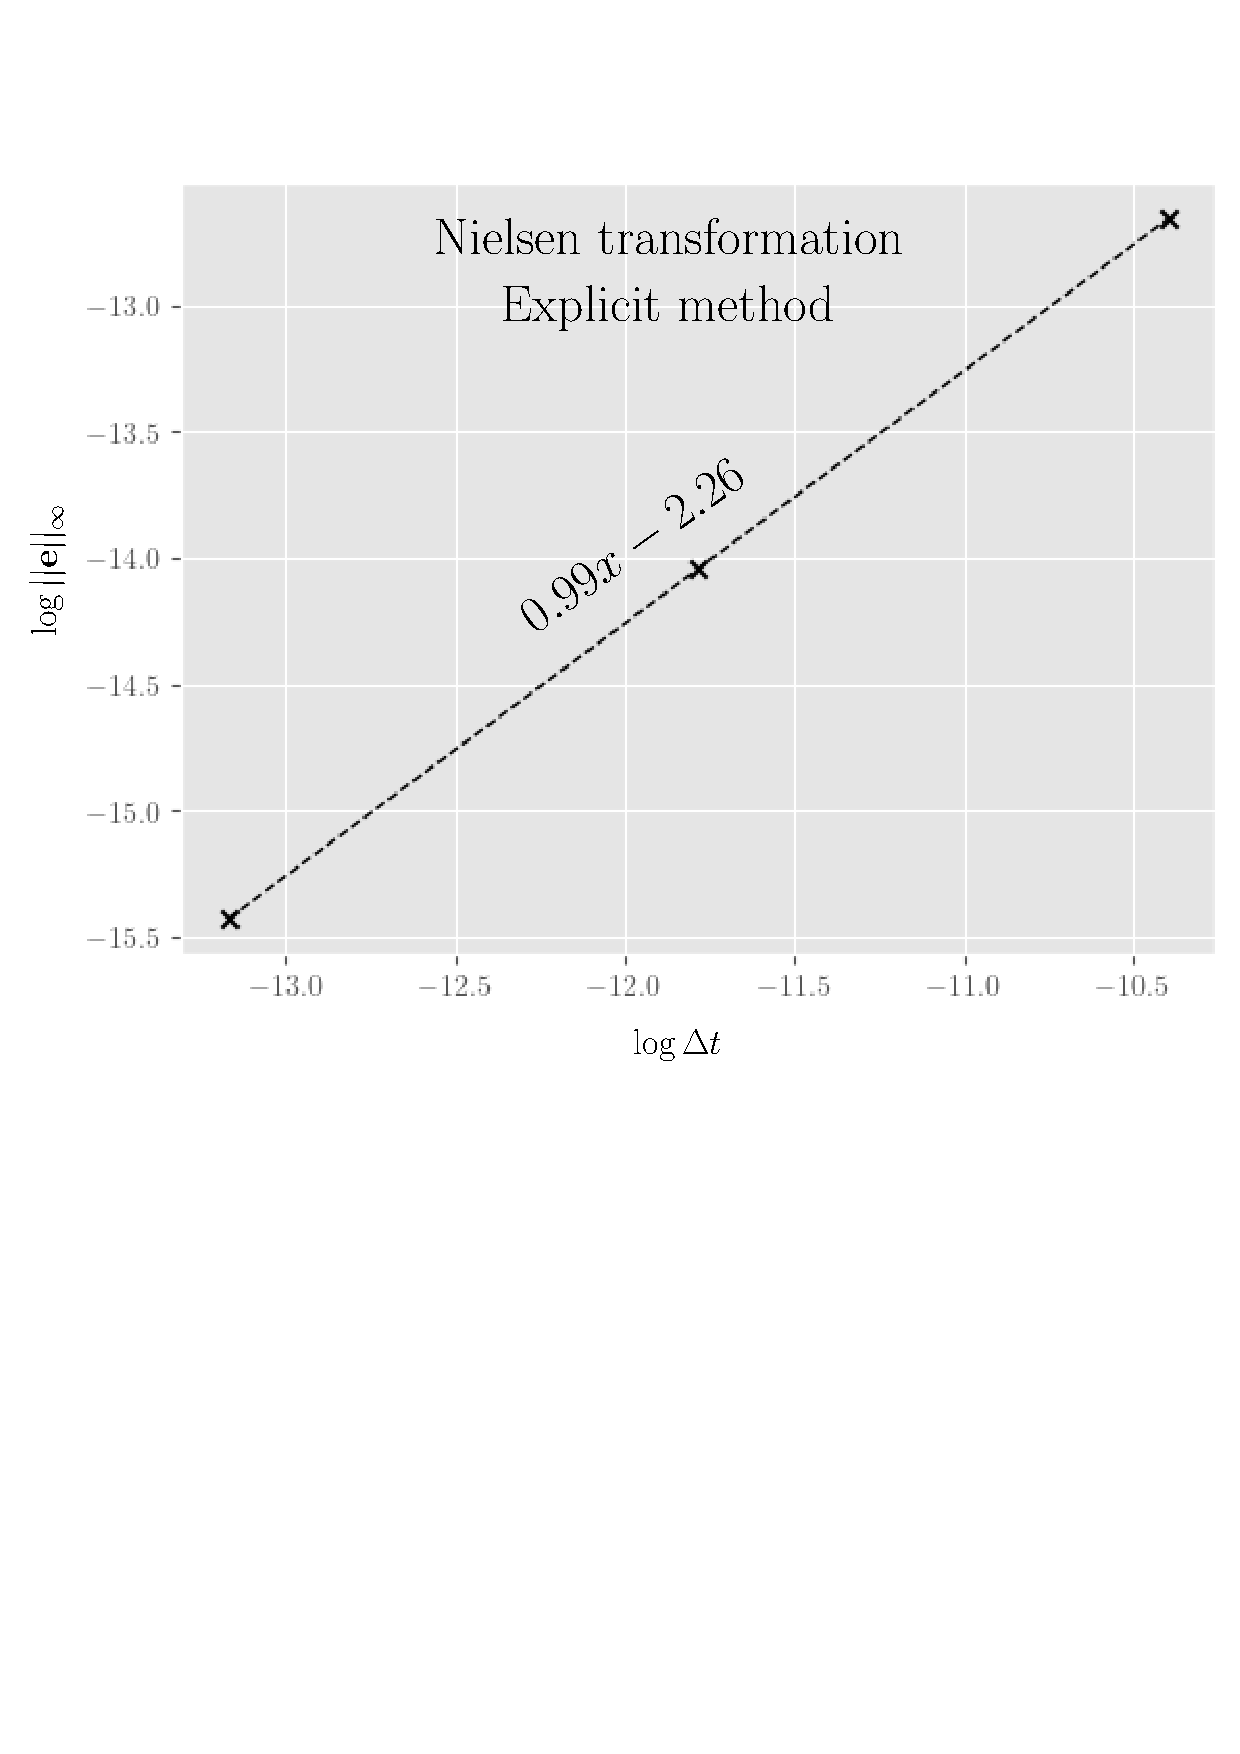
\includegraphics[width=\textwidth]{chapters/chapter3/ConvergenceTimeExplicitNielsen.pdf}
    \caption{$\Delta{t}=2^{-15},2^{-17},\dots,2^{-21}$}
    \caption*{$\Delta{x}=2^{-7}$}
    \label{fig:finitedifferencesschemes:numericaresults:nielsen_explicit_time}
  \end{subfigure}
  \begin{subfigure}{0.4\textwidth}
    \centering
    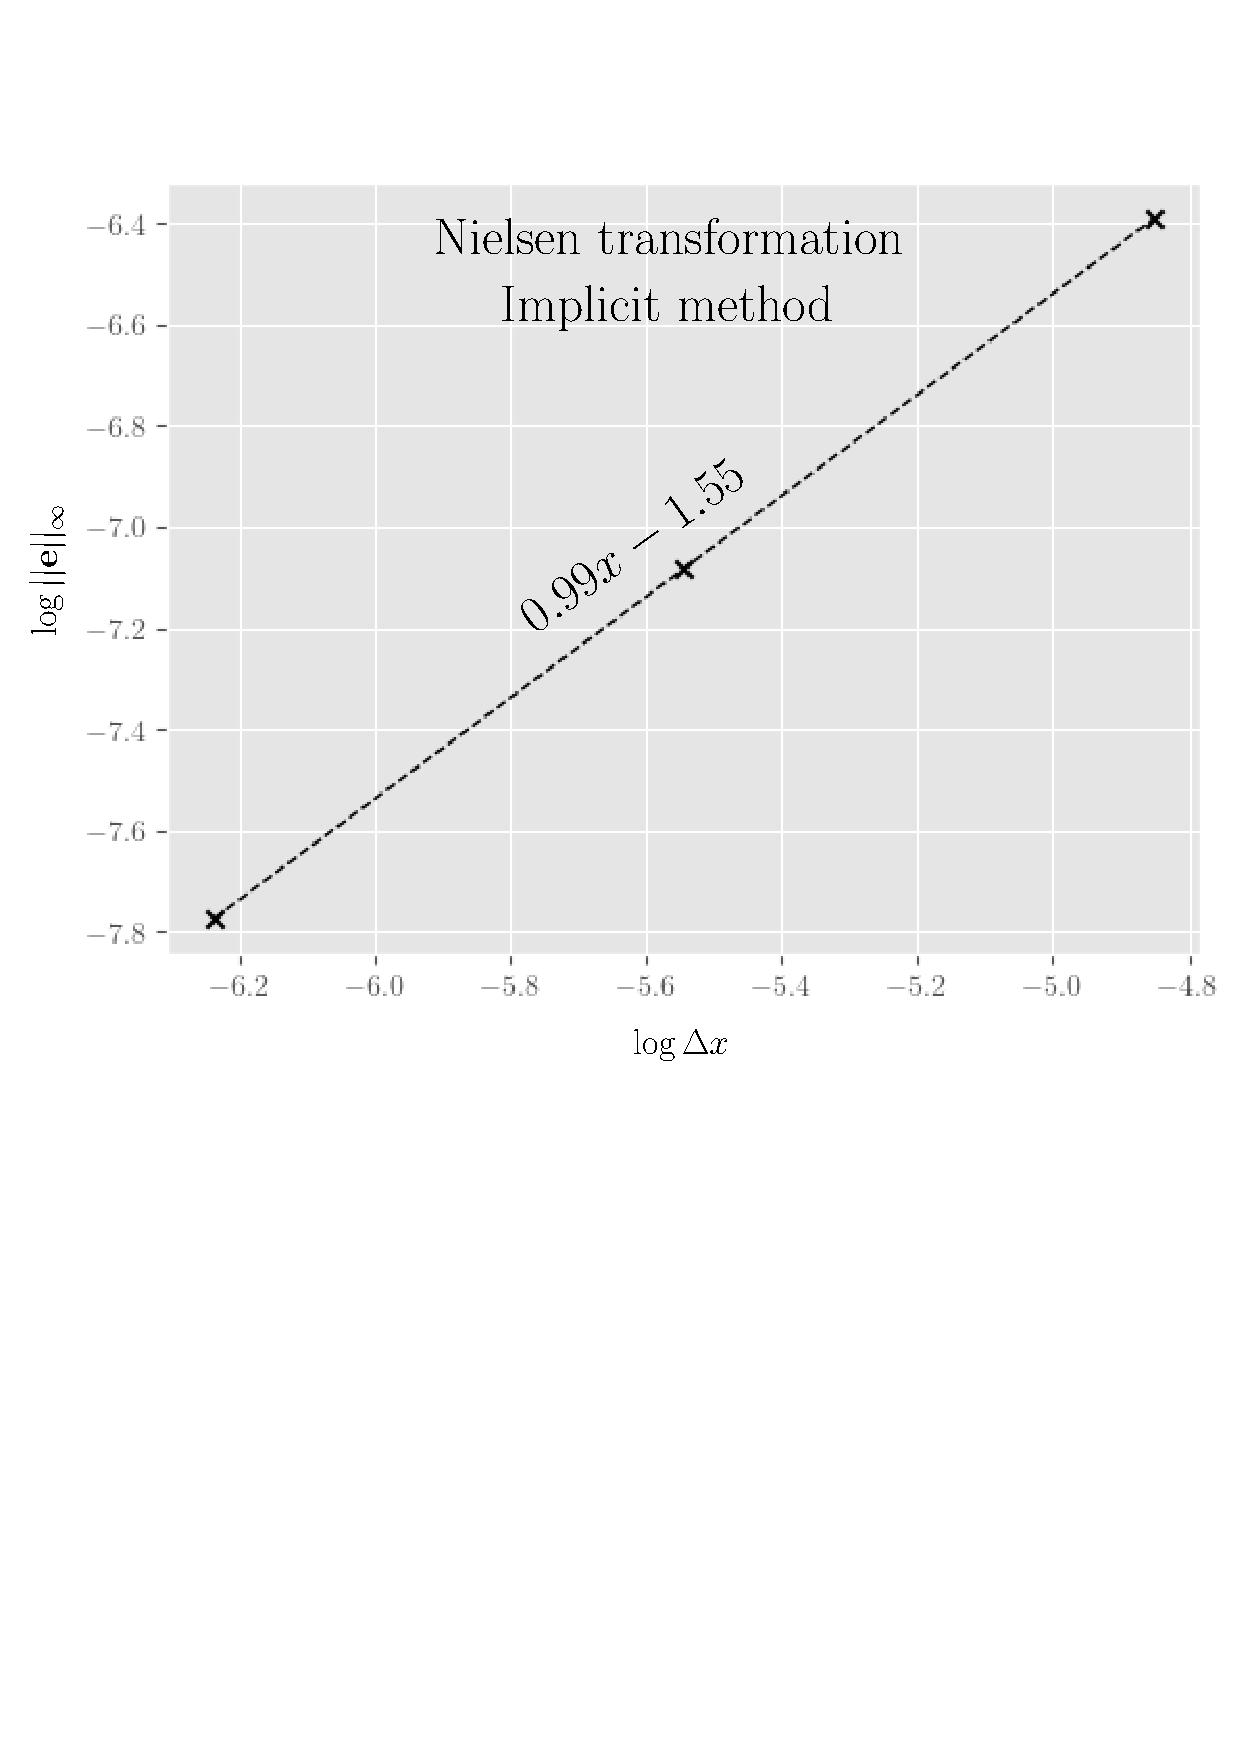
\includegraphics[width=\textwidth]{chapters/chapter3/ConvergenceSpaceImplicitNielsen.pdf}
    \caption{$\Delta{x}=2^{-6},\dots,2^{-8}$}
    \caption*{$\Delta{t}=2^{-2}$}
    \label{fig:finitedifferencesschemes:numericaresults:nielsen_implicit_space}
  \end{subfigure}
  \hspace{0.5cm}
  \begin{subfigure}{0.4\textwidth}
    \label{fig:finitedifferencesschemes:numericaresults:nielsen_implicit_time}
    \centering
    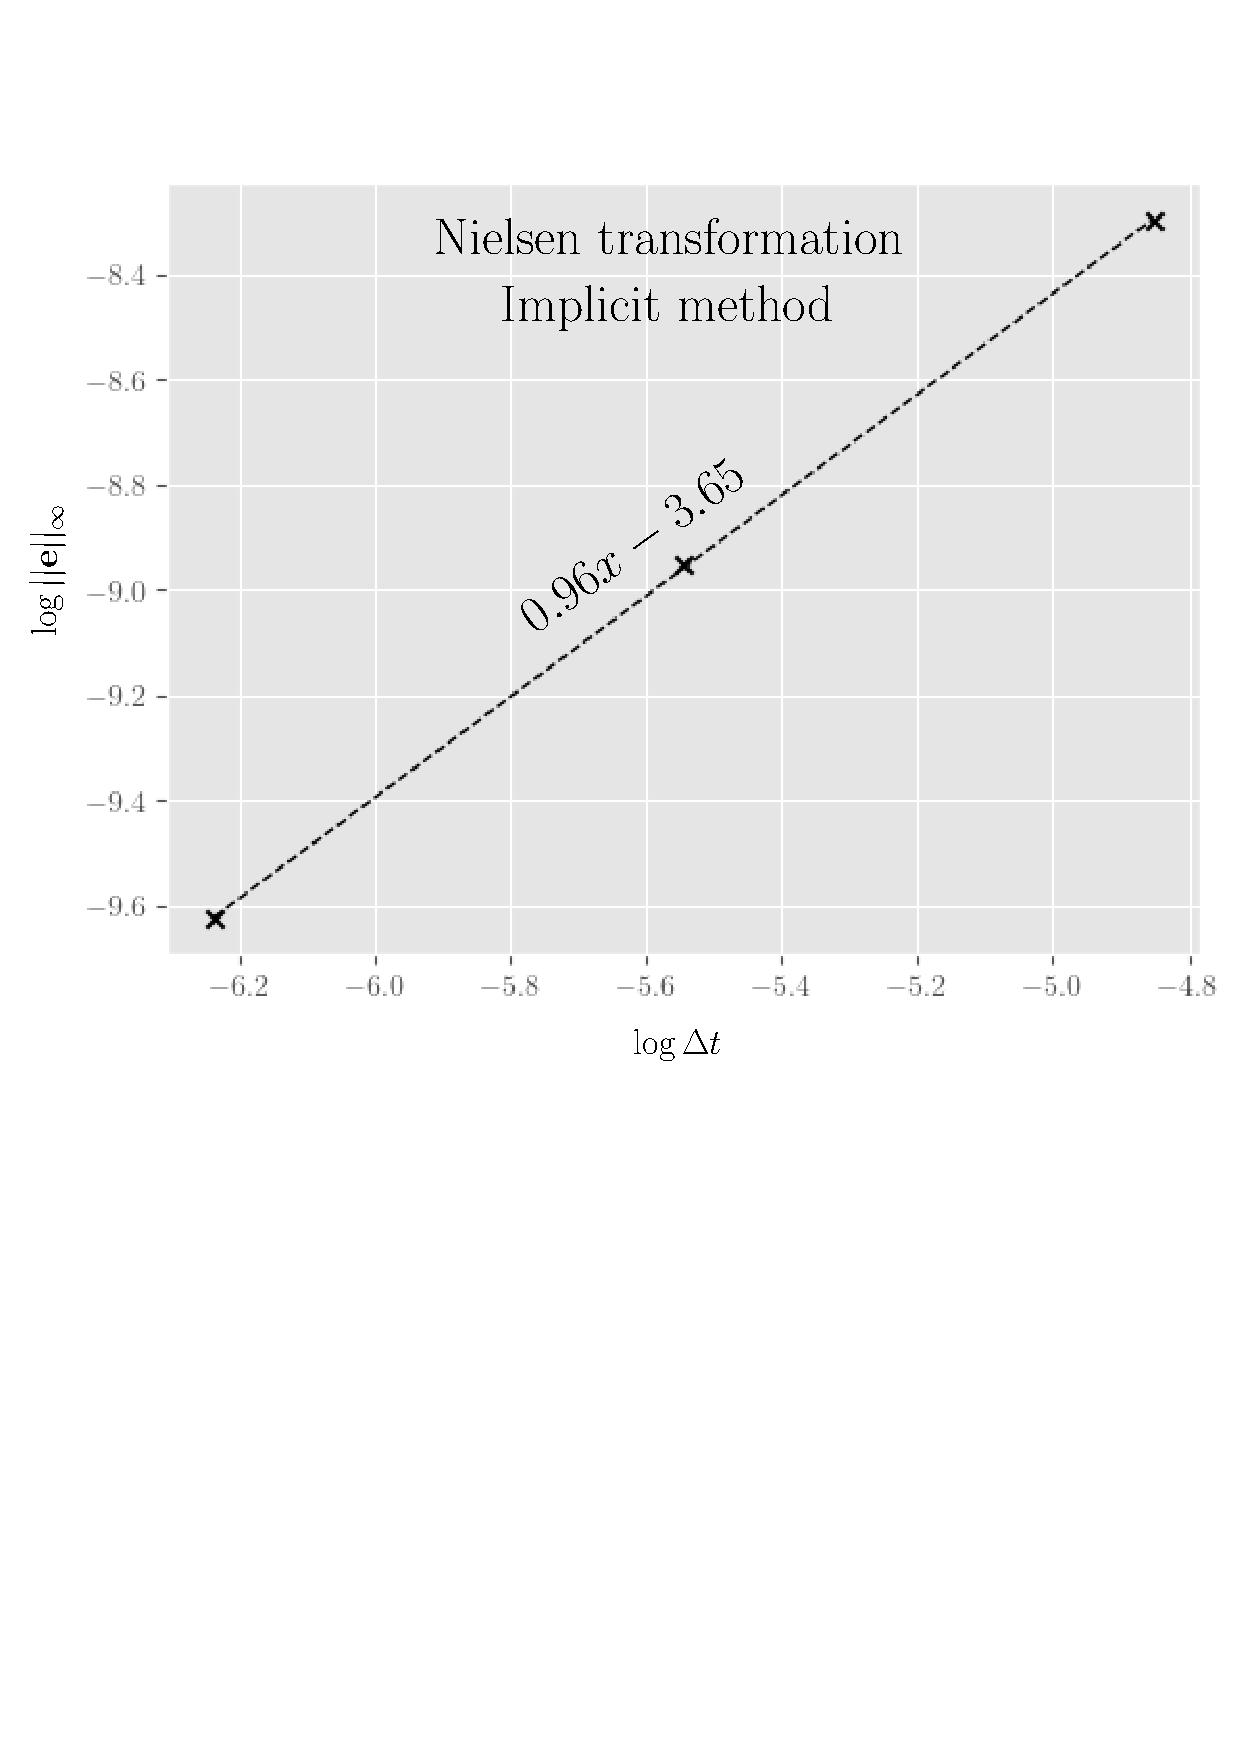
\includegraphics[width=\textwidth]{chapters/chapter3/ConvergenceTimeImplicitNielsen.pdf}
    \caption{$\Delta{t}=2^{-7},2^{-8},\dots,2^{-10}$}
    \caption*{$\Delta{x}=2^{-5}$}
  \end{subfigure}
  \caption{Convergence analysis for the explicit and implicit method for the Nielsen transformation.}
  \label{fig:finitedifferencesschemes:numericaresults:nielsen_convergence analysis}
\end{figure}

\begin{figure}[tbp]
  \centering
  \begin{subfigure}{0.4\textwidth}
    \centering
    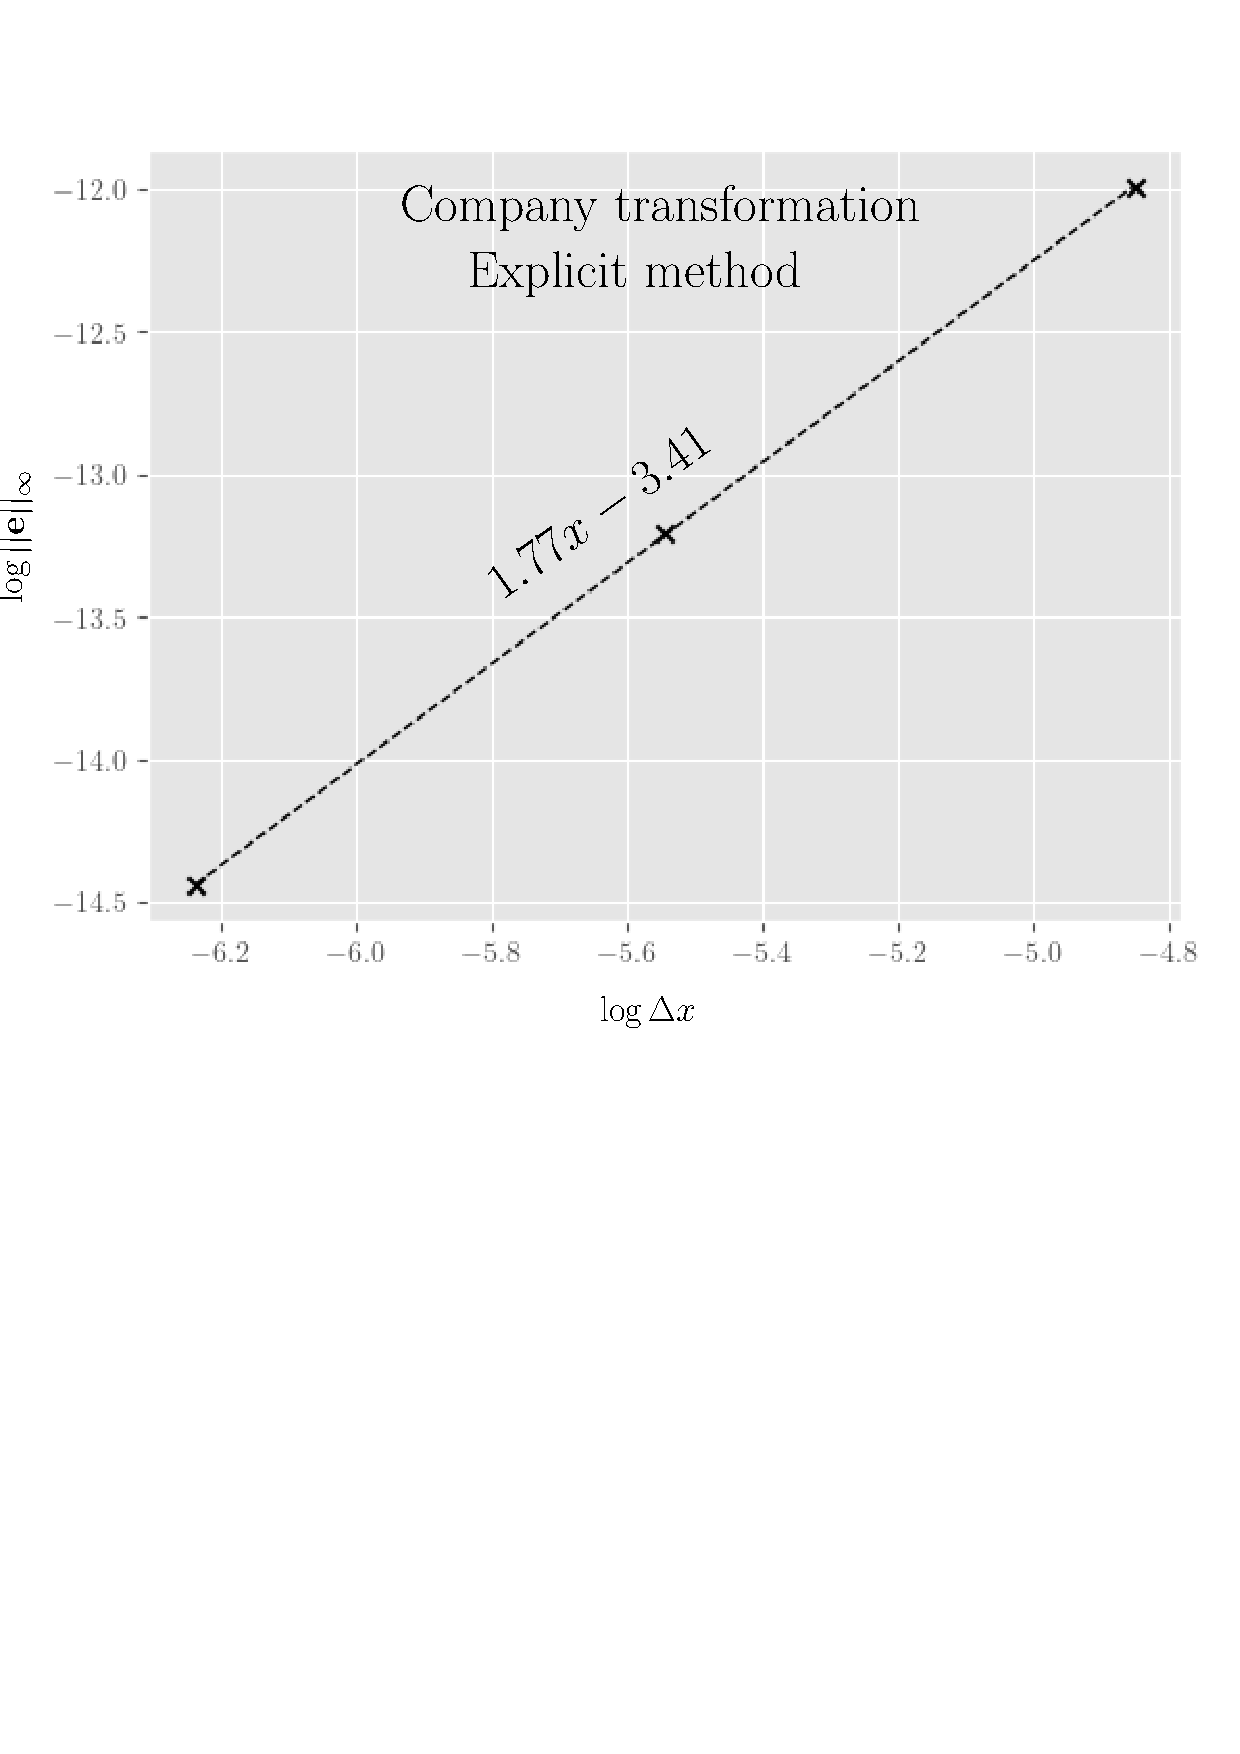
\includegraphics[width=\textwidth]{chapters/chapter3/ConvergenceSpaceExplicitCompany.pdf}
    \caption{$\Delta{x}=2^{-7},\dots,2^{-10}$}
    \caption*{$\Delta{t}=2^{-21}$}
    \label{fig:finitedifferencesschemes:numericaresults:company_explicit_space}
  \end{subfigure}
  \hspace{0.5cm}
  \begin{subfigure}{0.4\textwidth}
    \centering
    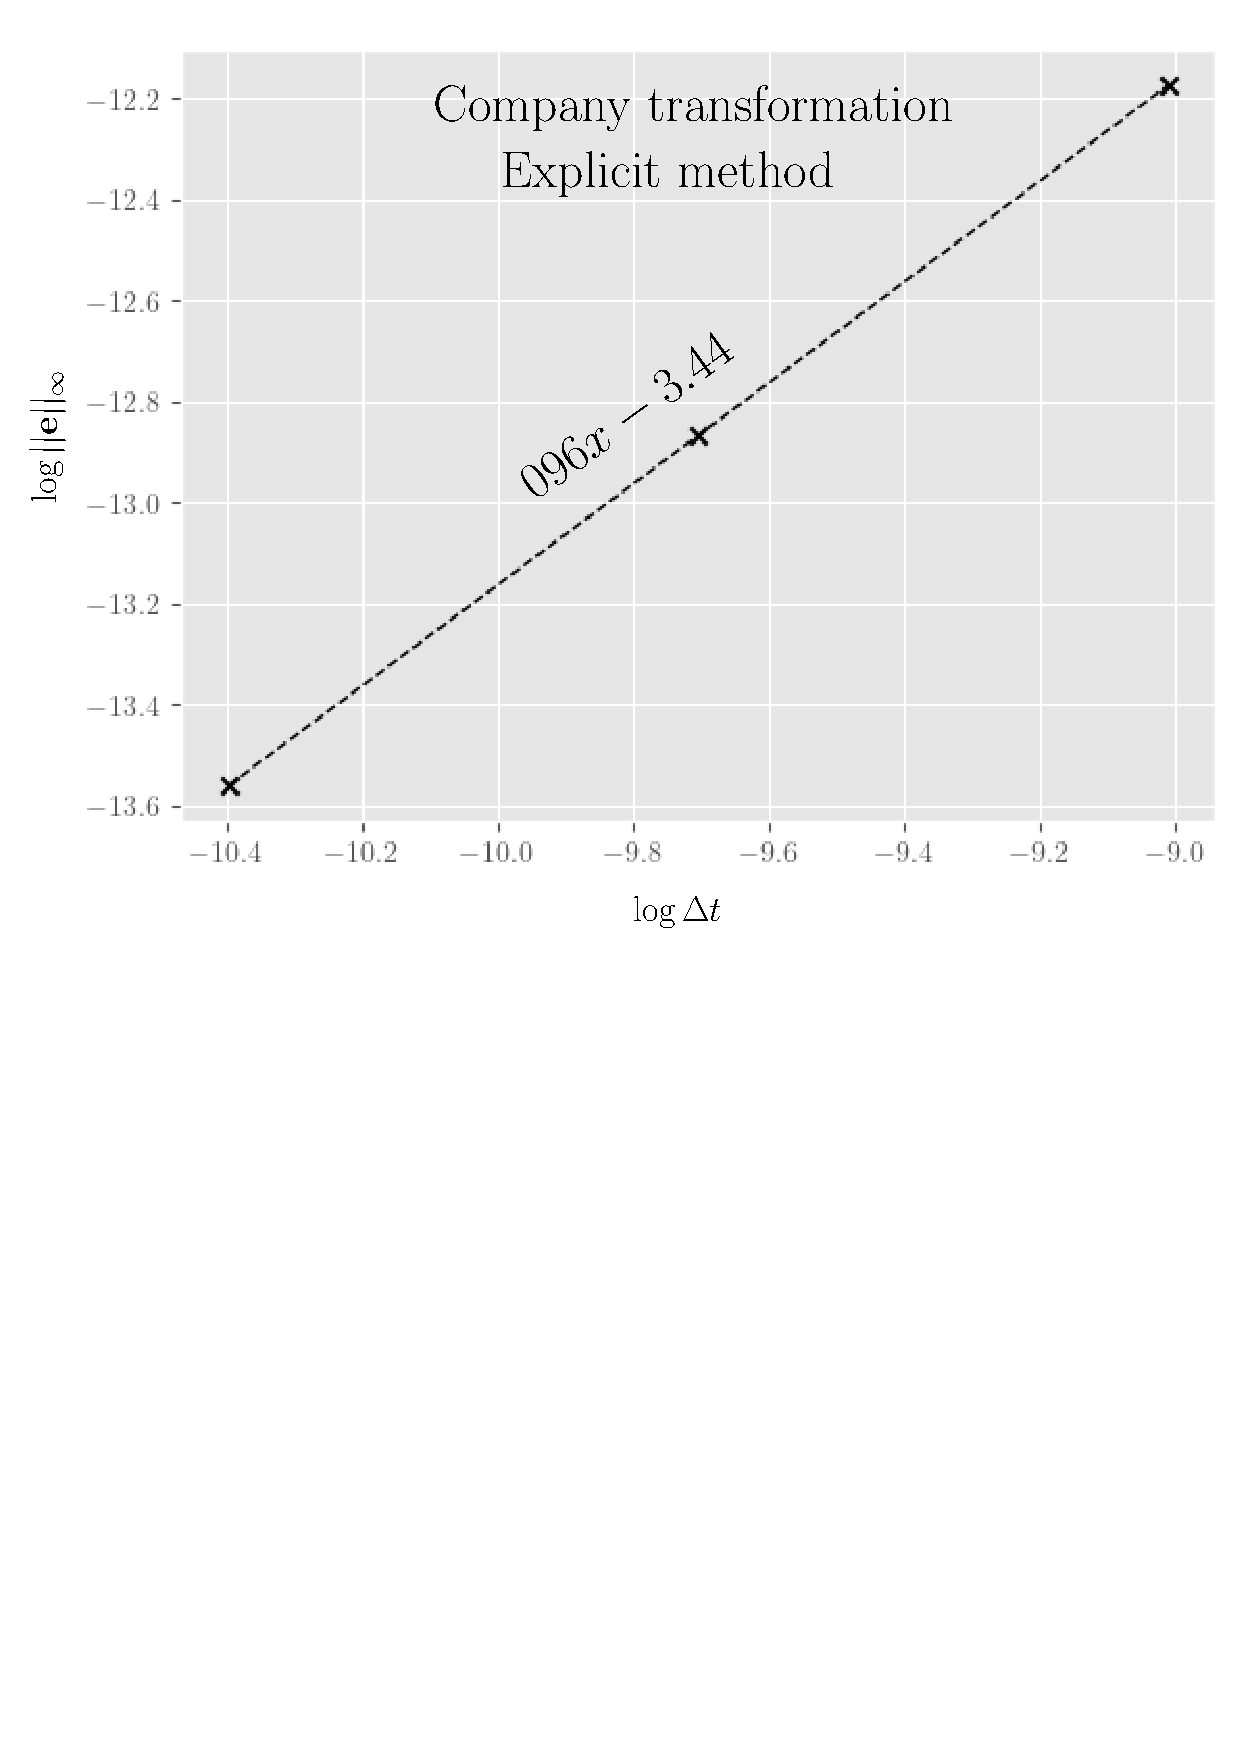
\includegraphics[width=\textwidth]{chapters/chapter3/ConvergenceTimeExplicitCompany.pdf}
    \caption{$\Delta{t}=2^{-15},2^{-17},\dots,2^{-21}$}
    \caption*{$\Delta{x}=2^{-7}$}
    \label{fig:finitedifferencesschemes:numericaresults:company_explicit_time}
  \end{subfigure}
  \caption{Convergence analysis for the explicit method for the Company transformation.}
  \label{fig:finitedifferencesschemes:numericaresults:company_convergence analysis}
\end{figure}